\documentclass[%
%draft,%
11pt,%
%oneside,%
twoside,%‡
%twocolumn,%
titlepage,%
%fleqn,%
%a4page,%
german,%
headsepline%
]{scrartcl}

%\usepackage{fancyhdr}
%\usepackage{scrpage}
\usepackage{lastpage}
\usepackage{geometry}
\usepackage{graphicx}
\usepackage[utf8]{inputenc}
\usepackage[ngerman]{babel}
\usepackage{lscape}
\usepackage[framemethod=TikZ]{mdframed}
\usepackage[most]{tcolorbox}
\usepackage{mymath}
\usepackage{units}
\usepackage{nicefrac}
\usepackage{pgf,tikz}
\usetikzlibrary{arrows}
\usepackage{colortbl}
\usepackage{hhline}
\usepackage{multirow}
\usepackage[extendedchars]{grffile}
\usepackage{caption}
\usepackage{multicol,calc}
\usepackage{blindtext}
\usepackage{pdfpages}
\usepackage{hyperref}
%\usepackage{tikz-er2}
\usepackage{framed}
\usetikzlibrary{arrows}
\usetikzlibrary{positioning}
\usetikzlibrary{shadows}

\usepackage{marginnote}
\usepackage
[draft]%
{qrcode}
\qrset{height=9ex}

%\usepackage{romannum}
\usepackage{longtable}
\usepackage{listings}
\usepackage{wrapfig}


% Command, um Tabellen-Spalten anzupassen
\newcommand{\spaltenheight}{\rule{0mm}{3ex}}
\newcommand{\spaltenwidth}{\rule{3cm}{0mm}}
\newcommand{\spaltensep}{\\[1ex]}
%\arrayrulecolor{darkgreen}
\doublerulesepcolor{white}
\definecolor{lightyellow}{rgb}{1,1,0.8}
\definecolor{Gray}{gray}{0.9}


% Pagestyle/Layout
%\geometry{a4paper , tmargin =2.5cm,	bmargin=3cm, lmargin =2.5cm,	rmargin =2.5cm,	headheight=3em, headsep=1em, footskip=1cm}
%\setlength{\parindent}{0pt} \setlength{\parskip}{1em}
%für TwoSide
%\lhead{\headmark\pagemark}
%\cehead{}
%\rehead{}
%\lohead{}
%\cohead{}
%\rohead{\headmark}
%für OneSide
%\ihead{}
%\chead{}
%\ohead{}
%\setheadsepline{0.5pt} % Linie zur Begrenzung
%\setfootsepline{0.5pt} % Linie zur Begrenzung
\pagestyle{headings} % gemachte Einstellungen anwenden

% Farbig umrahmte Umgebung Satz
 
 \definecolor{myblizzardblue}{HTML}{87CEEB}

\newcounter{satzz}[section]\setcounter{satzz}{0}
\renewcommand{\thesatz}{\arabic{section}.\arabic{satzz}}

\newenvironment{csatz}[2][]{%
    \refstepcounter{satzz}
 
    \ifstrempty{#1}%
    % if condition (without title)
    {\mdfsetup{%
        frametitle={%
            \tikz[baseline=(current bounding box.east),outer sep=0pt]
            \node[anchor=east,rectangle,fill=myblizzardblue]
            {\strut Satz~\thesatz};}
        }%
    % else condition (with title)
    }{\mdfsetup{%
        frametitle={%
            \tikz[baseline=(current bounding box.east),outer sep=0pt]
            \node[anchor=east,rectangle,fill=myblizzardblue]
            {\strut Satz~\thesatz:~#1};}%
        }%
    }%
% for both conditions
    \mdfsetup{%
        innertopmargin=10pt,linecolor=myblizzardblue,%
        backgroundcolor=whitesmoke,%
        linewidth=2pt,topline=true,%
        frametitleaboveskip=\dimexpr-\ht\strutbox\relax%
    }
 
\begin{mdframed}[]\relax}{%
\end{mdframed}}

% Farbig umrahmte Umgebung Theorem
 
\definecolor{mygraphblue}{HTML}{84B7E1}
\definecolor{whitesmoke}{HTML}{F5F5F5}

\newcounter{theo}[section]\setcounter{theo}{0}
\renewcommand{\thetheo}{\arabic{section}.\arabic{theo}}

\newenvironment{ctheo}[2][]{%
    \refstepcounter{theo}
 
    \ifstrempty{#1}%
    % if condition (without title)
    {\mdfsetup{%
        frametitle={%
            \tikz[baseline=(current bounding box.east),outer sep=0pt]
            \node[anchor=east,rectangle,fill=mygraphblue]
            {\strut Theorem~\thetheo};}
        }%
    % else condition (with title)
    }{\mdfsetup{%
        frametitle={%
            \tikz[baseline=(current bounding box.east),outer sep=0pt]
            \node[anchor=east,rectangle,fill=mygraphblue]
            {\strut Theorem~\thetheo:~#1};}%
        }%
    }%
% for both conditions
    \mdfsetup{%
        innertopmargin=10pt,linecolor=mygraphblue,%
        backgroundcolor=whitesmoke,%
        linewidth=2pt,topline=true,%
        frametitleaboveskip=\dimexpr-\ht\strutbox\relax%
    }
 
\begin{mdframed}[]\relax}{%
\end{mdframed}}

% Farbig umrahmte Umgebung Definition
 
 \definecolor{emerald}{HTML}{50C878}

\newcounter{deff}[section]\setcounter{deff}{0}
\renewcommand{\thedeff}{\arabic{section}.\arabic{deff}}

\newenvironment{cdef}[2][]{%
    \refstepcounter{deff}
 
    \ifstrempty{#1}%
    % if condition (without title)
    {\mdfsetup{%
        frametitle={%
            \tikz[baseline=(current bounding box.east),outer sep=0pt]
            \node[anchor=east,rectangle,fill=emerald]
            {\strut Definition~\thedeff};}
        }%
    % else condition (with title)
    }{\mdfsetup{%
        frametitle={%
            \tikz[baseline=(current bounding box.east),outer sep=0pt]
            \node[anchor=east,rectangle,fill=emerald]
            {\strut Definition~\thedeff:~#1};}%
        }%
    }%
% for both conditions
    \mdfsetup{%
        innertopmargin=10pt,linecolor=emerald,%
        backgroundcolor=whitesmoke,%
        linewidth=2pt,topline=true,%
        frametitleaboveskip=\dimexpr-\ht\strutbox\relax%
    }
 
\begin{mdframed}[]\relax}{%
\end{mdframed}}

% Farbig umrahmte Umgebung Achtung
 
 \definecolor{mygraphred}{HTML}{E26A6A}

\newcounter{merkee}[section]\setcounter{merkee}{0}
\renewcommand{\themerkee}{\arabic{section}.\arabic{merkee}}

\newenvironment{cachtung}[2][]{%
    \refstepcounter{merkee}
 
    \ifstrempty{#1}%
    % if condition (without title)
    {\mdfsetup{%
        frametitle={%
            \tikz[baseline=(current bounding box.east),outer sep=0pt]
            \node[anchor=east,rectangle,fill=mygraphred]
            {\strut Achtung};}
        }%
    % else condition (with title)
    }{\mdfsetup{%
        frametitle={%
            \tikz[baseline=(current bounding box.east),outer sep=0pt]
            \node[anchor=east,rectangle,fill=mygraphred]
            {\strut Achtung:~#1};}%
        }%
    }%
% for both conditions
    \mdfsetup{%
        innertopmargin=10pt,linecolor=mygraphred,%
        backgroundcolor=whitesmoke,%
        linewidth=2pt,topline=true,%
        frametitleaboveskip=\dimexpr-\ht\strutbox\relax%
    }
 
\begin{mdframed}[]\relax}{%
\end{mdframed}}

\subject{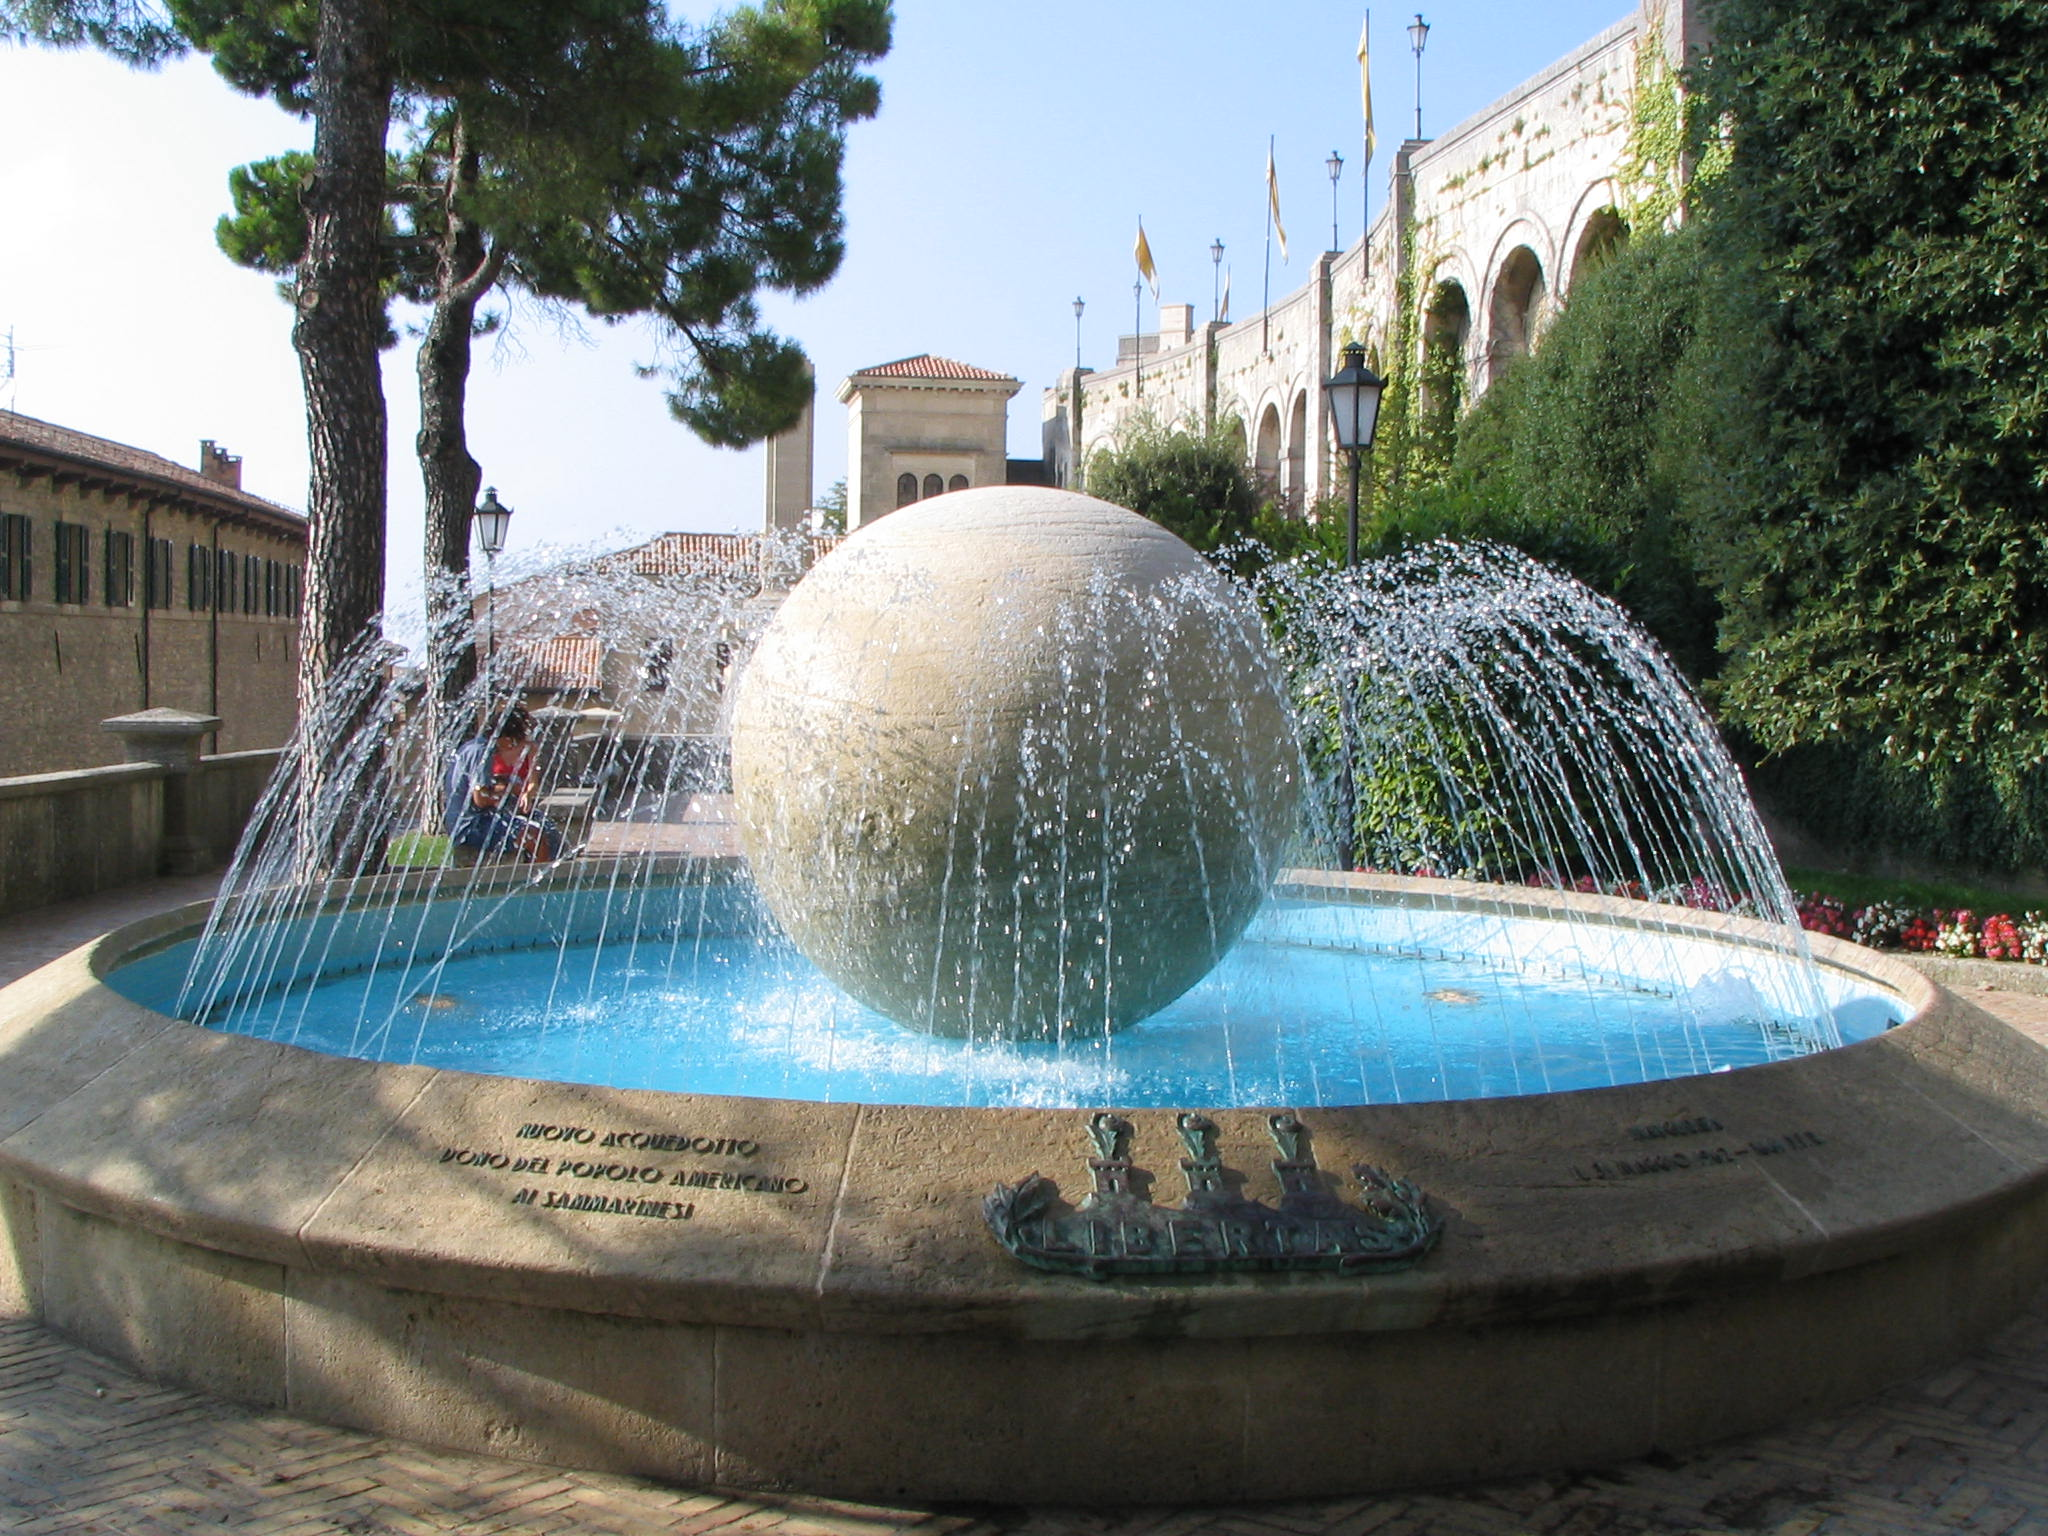
\includegraphics[width=0.618\textwidth]{pictures/springbrunnen.jpg}}
\title{Funktionentypen}
\subtitle{beyond linear}
\author{}
\date{}
\lowertitleback{

\includegraphics[height=3ex]{pictures/gymfmslerbermattlogo.eps}%
\hfill\copyright Jorma Wassmer
%1. Auflage, Februar 2011
}


\begin{document}
\maketitle
\tableofcontents
%\thispagestyle{empty}
\cleardoublepage
%\setcounter{page}{1}

\section{Einleitung}

Die QR-Codes am Computer können so benutzt werden, dass das Code-Quadrat mit gehaltener linker Maustaste in einen Browser gezogen wird.

\section{Der Funktionsbegriff}

\subsection{Funktionen}
In der Mathematik betrachtet man oft Abbildungen, bei denen die Zielmenge eine Zahlenmenge ist. Solche Abbildungen werden Funktionen genannt. Bei Funktionen ist es \"ublich, die Urbilder als Argumente, die Bilder als Funktionswerte, die Ausgangsmenge als Definitionsmenge und die Bildmenge als Wertemenge zu bezeichnen.
\begin{cdef}[Funktion]{}
Eine \emph{Funktion} $f$
\marginnote{
\qrcode{
https://www.youtube.com/watch?v=JMlfCH56rBk}
}
ist eine Abbildung, die jedem Element der Definitionsmenge \emph{genau ein} Element aus einer \emph{Zahlenmenge} zuordnet.
\end{cdef}
\begin{bem}
Falls nicht anders festgelegt, so sind Definitions- und Wertemenge gleich $\mR$.
\end{bem}
Der Funktionsbegriff ist f\"ur die Mathematik zentral, da er in den Naturwissenschaften, in der Technik, in den Wirtschaftswissenschaften und auch in vielen andern Wissensgebieten eine grosse Rolle spielt. Denn Funktionen bieten die M\"oglichkeit, Abh\"angigkeiten zwischen verschiedenen Gr\"ossen zu beschreiben.

\begin{bsp}
L\"asst man einen Stein vom Dach des schiefen Turms von Pisa fallen, so wird durch
$$h(t)=56-4.9t^2$$
die H\"ohe $h$ des Steins, in Metern \"uber dem Erdboden, $t$ Sekunden nach dem Fallenlassen beschrieben.
\end{bsp}

\begin{ueb}
Wie hoch ist der schiefe Turm von Pisa? Wie viele Meter \"uber dem Boden ist der Stein nach $2$ Sekunden Flugzeit? Wann trifft der Stein auf den Boden auf?
\end{ueb}

\begin{bsp}
Die Funktion, welche vorschreibt, eine Zahl zu quadrieren notieren wir kurz mit
$$f(x)=x^2.$$
Es ist dann beispielsweise $f(2)=2^2=4, f(0)=0^2=0, f(-3)=(-3)^2=9,\dots$. Praktisch ist h\"aufig die Illustration einer Funktion in einem Koordinatensystem. Man zeichnet also die Zahlenpaare $\point{2}{4}, \point{0}{0}, \point{-3}{9},\dots$.
\end{bsp}
\begin{bem}
In $y=f(x)$ heisst $x$ \emph{Argument von $f$} und $y$ bzw. $f(x)$ \emph{Wert von $f$}.
\end{bem}
\begin{ueb}[Funktionen]
Nenne Beispiele aus dem Alltag, denen Funktionen zugrunde liegen.
\end{ueb}
\begin{ueb}[Schreibweise]
Gegeben sei die Funktion
$$g(x)=x^2-2x+3$$
\begin{enumeratea}
\item Berechne $g(2),g(3),g(4)-g(-4),g(a^2)$.
\item F\"ur welchen Wert $x$ ist $g(x)=x^2,2,3$?
\end{enumeratea}
\end{ueb}
\begin{ueb}[Schreibweise 2]
Es sei
$$h(z)=z^3-z+2$$
Berechne $h(3),h(-1),h(0)$.
\end{ueb}
\begin{ueb}[Schreibweise 3]
Betrachte
$$s(t)=\frac{t+2}{t-1}$$
Berechne $s(0)$, $s(-2)$, $s(1)$, $s(10)$. F\"ur welche Argumente $t$ ist der Funktionswert $s(t)=1$, $2$, $-5$, $0$?
\end{ueb}
\begin{ueb}[Schreibweise 4]
Berechne f\"ur
$$f(x)=2^x-1$$
$f(1),f(3),f(10)$. An welcher Stelle wird der Funktionswert $31$?
\end{ueb}
\begin{ueb}[Zellteilung]
Ein Einzeller vermehrt sich alle 5 Minuten durch Zellteilung. Welche Funktion beschreibt diesen Sachverhalt? Nach welcher Zeit entwickeln sich aus einem Einzeller mehr als 1000 Zellen? Wie viele Zellen haben sich aus nur einem Einzeller nach $35$ Minuten entwickelt?
\end{ueb}
\begin{cdef}[Nullstelle]{}
Gilt
\marginnote{
\qrcode{
https://www.youtube.com/watch?v=-Ufvs3QlBXs}
}
f\"ur einen Wert $x$ der Definitionsmenge $f(x)=0$, so heisst $x$ \emph{Nullstelle} der Funktion $f$.
\end{cdef}
Nullstellen sind also --- wie der Name sagt --- diejenigen Stellen, an denen der Funktionswert gerade $0$ ist.
\begin{ueb}[Nullstellen]
Ermittle die maximale Definitionsmenge $\mD$, die minimale Wertemenge $\mW$ und die Nullstellen der Funktion $f:x\mapsto$\\

(a) $2x-6\q$ (b) $3x+1\q$ (c) $x^2\q$ (d) $\sqrt{x}\q$ (e) $x^3\q$ (f) $\frac{1}{x}\q$ (g) $x^2+1\q$ (h) $\sqrt{x-5}$
\end{ueb}

\begin{ueb}[Nullstellen 2]
Ermittle die Definitionsmenge $\mD$ und die Nullstellen der Funktion $f:x\mapsto$
  \\
  
  (a) $(x-2)(x+3)\q$ (b) $\frac{1}{x-4}\q$ (c) $x^2-7x+12\q$ (d) $(x+100)(x^2-49)\q$ (e) $\sqrt{x+6}$
\end{ueb}

\begin{ueb}[Schreibweise 5]
Dr\"ucke die folgenden Aussagen kurz und pr\"agnant in mathematischer Schreibweise aus:
\begin{enumeratea}
\item Durch die Funktion $f$ wird der Zahl $5$ die Zahl $132$ zugeordnet.
\item Die Funktion $h$ nimmt f\"ur $x=-2$ den Funktionswert $18$ an.
\item Die Zahl $7$ geh\"ort nicht zur Definitionsmenge der Funktion $f$.
\item Die Funktion $f$ ordnet der Zahl $3$ einen gr\"osseren Wert zu als der Zahl $8$.
\item Alle Funktionswerte der Funktion $f$ sind positiv.
\item Die Funktion $f$ nimmt jede positive Zahl als Funktionswert an.
\item Die Funktion $f$ ordnet jeder reellen Zahl das um $7$ vermehrte Quadrat dieser Zahl zu.
\item Die Funktion $f$ ordnet jeder reellen Zahl das Quadrat der um $3$ vergr\"osserten Zahl zu.
\item Die Funktion $f$ ordnet jeder reellen Zahl den um $13$ vergr\"osserten Kehrwert dieser Zahl zu.
\item Die Funktion $f$ ordnet jeder reellen Zahl den Kehrwert der um $4$ verminderten Zahl zu.
\end{enumeratea}
\end{ueb}

\begin{cdef}[Graph]{}
Sei
\marginnote{
\qrcode{
https://www.youtube.com/watch?v=gvtV3bGVE2U}
}
$f:\mD\longrightarrow\mW$ eine Funktion. Die Menge aller Punkte
$$\setm{\point{x}{y}}{y=f(x),x\in\mD}$$
heisst \emph{Graph} der Funktion $f$.
\end{cdef}
\begin{ueb}[Graph]
Zeichne den Graphen der Funk\-tion $f(x)=x^3$.
\end{ueb}

\begin{ueb}[Definition Funktion]
K\"onnen die folgenden Darstellungen Graphen von Funktionen sein? Woran erkennt man, ob eine Funktion dargestellt wird oder nicht?
\begin{center}
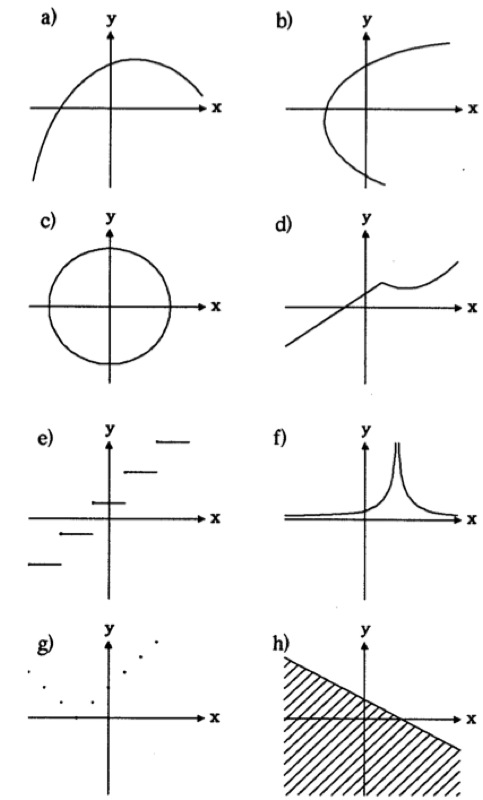
\includegraphics[width=0.618\textwidth]{pictures/graphen}
\end{center}
\end{ueb}

\subsection{Inversfunktionen}
\begin{wrapfigure}{r}{0.4\textwidth}
  \begin{center}
    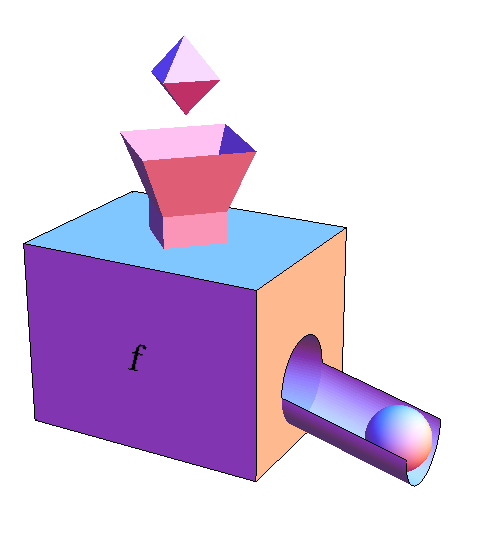
\includegraphics[width=0.15\textwidth]{pictures/maschine}
  \end{center}
%\caption{You Know my Name}
\end{wrapfigure}
Durch die Funktionsvorschrift
$$f(x)=2x-3$$
ist jedem $x$ genau ein $y$-Wert zugeordnet.

\begin{ueb}
Wie sieht der Graph von $f$ aus?
\end{ueb}
Umgekehrt ist in diesem Fall durch $f$ eine Funktion $f^{-1}$ definiert, die jedem Funktionswert $y$ genau einen $x$-Wert zuordnet.
\begin{ueb}[Wertetabelle]
Veranschauliche dir diesen Zusammenhang anhand einer Wertetabelle f\"ur die obige Funktion.
\end{ueb}
\begin{cdef}[Inversfunktion]{}
Gilt
\marginnote{
\qrcode{
https://www.youtube.com/watch?v=0ob7n10ZCC0}
}
f\"ur eine Funktion $f$
$$x_1\neq x_2\implies f(x_1)\neq f(x_2)$$
dann heisst $f^{-1}$ mit $f^{-1}(f(x))=x$ die \emph{Inversfunktion} von $f$
.
\end{cdef}
\begin{bem}
Die Voraussetzung, dass $f$ \emph{injektiv} ist, ist wesentlich.
\end{bem}
\begin{cdef}[Injektivität]{}
Eine
\marginnote{
\qrcode{
https://www.youtube.com/watch?v=1vkU9R7XBho}
}
Funktion heisst \emph{injektiv}
, wenn es zu jedem $y\in\mW$ \emph{h\"ochstens ein} $x\in\mD$ gibt.
\end{cdef}
\begin{ueb}[Injektivit\"at]
\"Uberzeuge dich davon, dass f\"ur eine Funktion
$$f:\mD\longrightarrow\mW$$
mit $x_1,x_2\in\mD$ die Definition von \glqq injektiv\grqq\ \"aquivalent zur Aussage
$$x_1\neq x_2\implies f(x_1)\neq f(x_2)$$
ist.
\end{ueb}
\begin{ueb}[Injektivit\"at 2]
Kann man, ausgehend von der Funktion
$$f(x)=x^2,\qq\mD=\mR,$$
eine Inversfunktion angeben?
\end{ueb}
\begin{bem}
Man findet den Funktionsterm von $f^{-1}$ in dem man die Gleichung
$$f(x)=y$$
nach $x$ aufl\"ost. Anschliessend vertauscht man noch die Bezeichnung $y$ mit $x$, weil \"ubli\-cher\-wei\-se $x$ die freie Variable darstellt und man daf\"ur die horizontale Achse verwenden will.
\end{bem}
\begin{bsp}
Die
\marginnote{
\qrcode{
https://www.youtube.com/watch?v=LvMvYokuueY}
}
Inversfunktion zu
$$f(x)=3x-2$$ ist demnach
\begin{align}
y&=3x-2\tag{$+2$}\\
y+2&=3x\tag{$\div3$}\\
\frac{y+2}{3}&=x\notag\\
f^{-1}(x)&=\frac{x+2}{3}=\frac{1}{3}x+\frac{2}{3}\notag\end{align}
\end{bsp}
\begin{ueb}[Spiegelung]
Zeichne die Graphen von $f$ und $f^{-1}$ aus dem Ein\-f\"uh\-rungs\-bei\-spiel in dasselbe Koordinatensystem, nachdem du den Funktionsterm von $f^{-1}$ gefunden hast.
\end{ueb}
\begin{ueb}[Winkelhalbierende]
Zeige, dass der Graph von $f^{-1}$ Spiegelbild des Graphen von $f$ an der Winkelhalbierenden $y=x$ durch den ersten und dritten Quadranten ist.

Hint: Betrachte einen beliebigen Punkt auf dem Graphen von $f$ und sein Pendant auf dem Graphen von $f^{-1}$. Skizziere diese Situation und argumentiere geometrisch.
\label{invsym}
\end{ueb}
\begin{csatz}[Achsensymmetrie der Inversfunktion]{}
Die Graphen von $f$ und $f^{-1}$ sind achsialsymmetrisch bez\"uglich der Winkelhalbierenden durch den ersten und dritten Quadranten.
\end{csatz}
\begin{proof}[Beweis]
Siehe \"Ubung \ref{invsym}
\end{proof}

\subsection{Der Differenzenquotient}
Manchmal ist man an der \"Anderung einer Funktion interessiert. Beispielsweise ist die Schwankung des SMI \"uber einen Tag oder sogar nur \"uber einen Monat relevant. Wie die Schwankungen tags\"uber verliefen, ist f\"ur den Aktienanleger unbedeutend. Also betrachtet man die \"Anderung einer Gr\"osse \"uber einem bestimmten Zeitabschnitt. Dabei vergleicht man Anfangs- und Endwert bez\"uglich der Dauer der Beobachtung.
\begin{cdef}[Differenzenquotient]
Der
\marginnote{
\qrcode{
https://www.youtube.com/watch?v=J0FCAuTM9pA}
}
Quotient
$$\frac{\Delta f(x)}{\Delta x}=\frac{f(x_2)-f(x_1)}{x_2-x_1}$$
gibt die durchschnittliche \"Anderung der Funktion im Intervall $[x_1,x_2]$ an. Diesen Quotienten nennt man \emph{Differenzenquotienten}
.
\end{cdef}

\begin{figure}
\definecolor{qqwuqq}{rgb}{0,0.39,0}
\definecolor{zzqqqq}{rgb}{0.6,0,0}
\definecolor{qqqqzz}{rgb}{0,0,0.6}
\definecolor{xdxdff}{rgb}{0.49,0.49,1}
\begin{center}
\begin{tikzpicture}[line cap=round,line join=round,>=triangle 45,x=0.6cm,y=0.4cm]
\draw[->,color=black] (-2.14,0) -- (12.34,0);
\foreach \x in {-2,-1,1,2,3,4,5,6,7,8,9,10,11}
\draw[shift={(\x,0)},color=black] (0pt,2pt) -- (0pt,-2pt);
\draw[->,color=black] (0,-1.96) -- (0,12);
\foreach \y in {-1,1,2,3,4,5,6,7,8,9,10,11}
\draw[shift={(0,\y)},color=black] (2pt,0pt) -- (-2pt,0pt);
\clip(-2.5,-1.96) rectangle (14.34,12);
\draw [shift={(8.5,4)},color=qqwuqq,fill=qqwuqq,fill opacity=0.1] (0,0) -- (90:0.6) arc (90:180:0.6) -- cycle;
\draw[line width=1.2pt, smooth,samples=100,domain=-2.1399999999999997:14.339999999999998] plot(\x,{0.5*(\x-5)^2+2});
\draw (3,4)-- (8.5,8.13);
\draw [line width=1.2pt,dotted,color=qqqqzz] (8.5,8.13)-- (8.5,0);
\draw [line width=1.2pt,dotted,color=qqqqzz] (3,0)-- (3,4);
\draw [line width=1.2pt,dotted,color=qqqqzz] (0,4)-- (3,4);
\draw [line width=1.2pt,dotted,color=qqqqzz] (0,8.13)-- (8.5,8.13);
\draw [line width=1.2pt,dash pattern=on 5pt off 5pt,color=zzqqqq] (3,4)-- (8.5,4);
\draw [line width=1.2pt,dash pattern=on 5pt off 5pt,color=zzqqqq] (8.5,4)-- (8.5,8.13);
\fill[color=qqwuqq,fill=qqwuqq,fill opacity=0.1] (8.25,4.25) circle (0.02);
\draw (2.5,-0.06) node[anchor=north west] {$x_1$};
\draw (8,-0.04) node[anchor=north west] {$x_2$};
\draw (-2.5,5) node[anchor=north west] {$f(x_1)$};
\draw (-2.5,8.8) node[anchor=north west] {$f(x_2)$};
\draw (8.5,6.4) node[anchor=north west] {$\Delta f$};
\draw (4.5,3.9) node[anchor=north west] {$\Delta x$};
\draw[color=black] (1.16,10.96) node {$f$};
\draw (11.5,1.2) node[anchor=north west] {$x$};
\draw (-1,12) node[anchor=north west] {$y$};
\fill [color=xdxdff] (3,4) circle (1.5pt);
%\draw[color=xdxdff] (2.1,3.5) node {$A$};
\fill [color=xdxdff] (8.6,8.13) circle (1.5pt);
%\draw[color=xdxdff] (9,8.2) node {$B$};
\end{tikzpicture}
\end{center}
\caption{Durchschnittliche \"Anderungsrate}
\end{figure}

\begin{cdef}[Intervall]{}
Die Menge
$$\setm{x\in\mR}{x_1\leq x \leq x_2}$$
wird \emph{Intervall} genannt und mit $[x_1,x_2]$ bezeichnet. Selbstverst\"andlich muss der Funktionswert an jeder Stelle des Intervalls definiert sein, d.h. das Intervall ist eine Teilmenge der De\-fi\-ni\-tions\-menge von $f$.
\end{cdef}

\begin{ueb}
Berechne die durchschnittliche \"Anderung der Funktion $f:x\mapsto$
\begin{enumeratea}
\item $x^2$ \"uber $[0,1],[2,3],[0,3],[-2,-1],[x_1,x_2]$
\item $\frac{1}{x}$ \"uber $[0.5,2],[-7,-2],[-1,1],[x_1,x_2]$
\item $x^2-2x+1$ \"uber $[-3,4],[0,6],[-2,2]$
\end{enumeratea}
\label{aenderung}
\end{ueb}

\begin{ueb}
Die Tabelle zeigt die Tarif- und Lebenskostenindizes (Index $1977\sim100$) f\"ur die Schweiz.
\begin{center}
\large
\begin{tabular}{|c|c|c|c|}
\hline
 & Fahrpreis Bahn & Gesamtlohnindex & Konsumentenpreise\\ \hline
1977 & 100 & 100 & 100\\ \hline
1979 & 101.5 & 106.6 & 104.4\\ \hline
1980 & 102.6 & 112.3 & 108.6\\ \hline
1981 & 107.9 & 119.3 & 115.7\\ \hline
1982 & 115.4 & 127.7 & 122.2\\ \hline
1983 & 125.1 & 132.5 & 125.8\\ \hline
1984 & 128.8 & 136.2 & 129.5\\ \hline
1985 & 131.1 & 140.4 & 133.9\\ \hline
1986 & 133.3 & 145.4 & 135.0\\ \hline
1987 & 130.3 & 148.9 & 137.0\\ \hline
1988 & 130.2 & 154.1 & 139.5\\ \hline
\end{tabular}
\end{center}
\begin{enumeratea}
\item Zeichne farbig in dasselbe Koordinatensystem die Graphen der Funktionen, die durch diese Tabelle dargestellt werden.
\item Berechne die durchschnittliche \"Anderung der drei Funktionen in den Intervallen $[1977,1988]$ und $[1986,1988]$.
\end{enumeratea}
\end{ueb}

\begin{cdef}[Monotonie]{}
Eine Funktion $f$ heisst \emph{monoton wachsend} im Intervall $I$, wenn die durchschnittliche \"Anderung f\"ur jedes Teilintervall von $I$ positiv oder Null ist. Entsprechend nennt man $f$ \emph{monoton fallend}, wenn f\"ur jedes Teilintervall von $I$ die durchschnittliche \"Anderung negativ oder Null ist.
\end{cdef}

\begin{ueb}
In welchen Intervallen sind die Funktionen aus \"Ubung \ref{aenderung} monoton wachsend, monoton fallend?
\end{ueb}

\cleardoublepage

\section{Quadratische Funktionen}

\subsection{Erste Beobachtungen}

\begin{wrapfigure}{r}{0.382\textwidth}
  \begin{center}
    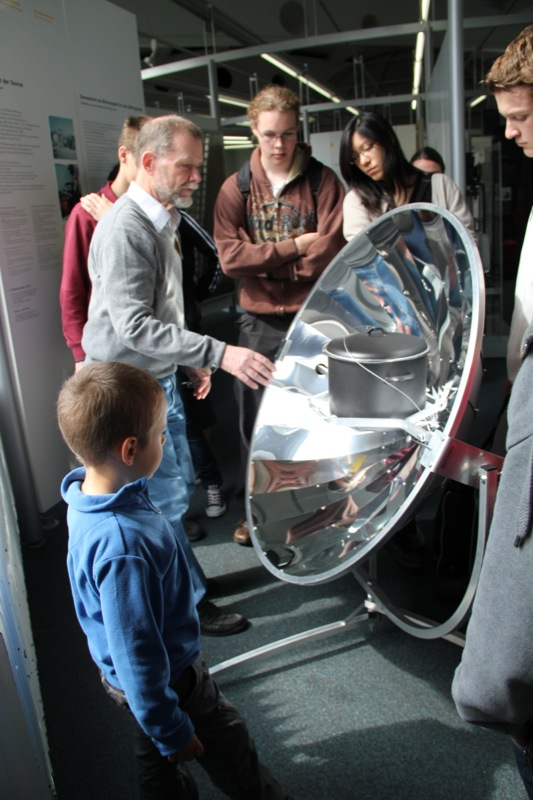
\includegraphics[width=0.382\textwidth]{pictures/parabol}
  \end{center}
\end{wrapfigure}
Quadratische Funktionen, beziehungsweise die Graphen davon, haben bemerkenswerte Eigenschaften. Im Folgenden wollen wir zuerst ein Beispiel anschauen, das die Grundlage vieler Anwendungen im Alltag illustriert. Anschliessend wird auf die Mathematik von quadratischen Funktionen und ihren Graphen eingegangen.
\begin{bsp}
Stellen Sie sich den unten abgebildeten Graphen der Funktion
$$f(x) = \frac{1}{4}x^2$$
als Spiegel vor. Zeichnen Sie vier parallel zur y-Achse einfallende Lichtstrahlen und konstruieren Sie ihre Reflexion. Beachten Sie dabei, dass die Tangente an den Graphen von $f$ an der Stelle $x$ die Steigung $\frac{1}{2}x$ hat.
\begin{figure}
\begin{center}
\definecolor{cqcqcq}{rgb}{0.75,0.75,0.75}
\begin{tikzpicture}[line cap=round,line join=round,>=triangle 45,x=0.75cm,y=0.75cm]
\draw [color=cqcqcq,dash pattern=on 2pt off 2pt, xstep=0.5cm,ystep=0.5cm] (-5.96,-2.6) grid (6.82,7.9);
\draw[->,color=black] (-5.96,0) -- (6.82,0);
\foreach \x in {-5,-4,-3,-2,-1,1,2,3,4,5,6}
\draw[shift={(\x,0)},color=black] (0pt,2pt) -- (0pt,-2pt) node[below] {\footnotesize $\x$};
\draw[color=black] (6.48,0.08) node [anchor=south west] {$x$};
\draw[->,color=black] (0,-2.6) -- (0,8.02);
\foreach \y in {-2,-1,1,2,3,4,5,6,7}
\draw[shift={(0,\y)},color=black] (2pt,0pt) -- (-2pt,0pt) node[left] {\footnotesize $\y$};
\draw[color=black] (0.1,7.62) node [anchor=west] {$y$};
\clip(-5.96,-2.6) rectangle (6.82,8.02);
\draw[line width=2pt, smooth,samples=100,domain=-5.96:6.82] plot(\x,{0.25*\x*\x});
\draw (0.6,6.5) node[anchor=north west] {$f(x)=\frac{1}{4}x^2$};
\end{tikzpicture}
\end{center}
\end{figure}
\end{bsp}
Beispiel 1 zeigt die wichtigste Eigenschaft der Graphen von quadratischen Funktionen. Alle parallel zur $y$-Achse einfallenden Strahlen werden in ein und denselben Punkt reflektiert. Dieser ausgezeichnete Punkt hat nat"urlich einen eigenen Namen verdient: man nennt ihn
\marginnote{
\qrcode{
https://www.youtube.com/watch?v=qcC-Bsrui1Y}
}
\emph{Brennpunkt}.
Tats\"achlich kann es dort sehr sehr heiss werden! Abbildung \ref{odiello} zeigt den gr\"ossten Parabolspiegel der Welt, welcher zu Forschungszwecken dient und das Sonnenlicht \glqq b"undelt\grqq. Damit werden im H\"auschen, das im Brennpunkt steht, Temperaturen bis zu $\unit[4000]{ ^\circ C}$ erreicht.

\begin{figure}
\begin{center}
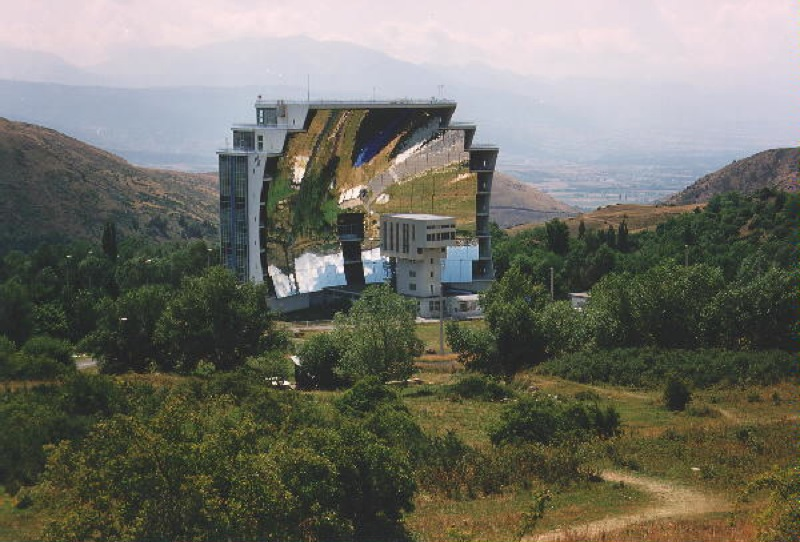
\includegraphics[width=0.618\textwidth]{pictures/odeillo}
\end{center}
\caption{Parabolspiegel in Odeillo}\label{odiello} 
\end{figure}

\subsection{Begriffe und Mathematik}
\begin{cdef}[Quadratische Funktion]{}
Eine
\marginnote{
\qrcode{
https://www.youtube.com/watch?v=FviMrIW3_0Q}
}
Funktion heisst \emph{quadratisch}, wenn sie sich mit einer Funktionsgleichung der Form
$$f(x) = ax^2+bx+c\q(a\neq0)$$
darstellen l\"asst.
\end{cdef}

\begin{bem}
Spezialfall: Funktionen der Form
$$f(x) = ax^2$$
haben die bequeme Eigenschaft, dass ihr Graph durch den Ursprung geht und dort, je nachdem ob $a>0$ oder $a<0$ ist, ihren Tief- bzw. Hochpunkt haben.
\end{bem}

\begin{ueb}[Graphen]
Zeichne in dasselbe Koordinatensystem die Graphen der Funktionen $f:x\mapsto$
\begin{enumeratea}
\item $x^2, \frac{1}{2}x^2, 2x^2, -\frac{1}{4}x^2$
\item $x^2+1, -x^2+1, \frac{1}{2}x^2-2, -2x^2+3, \frac{1}{5}x^2-1$
\end{enumeratea}
\end{ueb}

\begin{cdef}[Parabel und Scheitelpunkt]{}
Der
Graph einer quadratischen Funktionen nennt man \emph{Parabel}. Der Tief- bzw. Hochpunkt heisst \emph{Scheitel}.
\end{cdef}

\begin{csatz}[Brennpunkteigenschaft]{}
Die Parabel der Funktion
$$f(x)=ax^2$$
ist achsialsymmetrisch zur $y$-Achse. Die $x$-Achse ist Tangente im Scheitel. Jeder parallel zur $y$-Achse einfallende Lichtstrahl wird an der Parabel so gespiegelt, dass er durch den Brennpunkt geht.
\end{csatz}

\begin{proof}[Beweis]
Sp\"ater.
\end{proof}

\begin{csatz}[Symmetrie]{}
Der Scheitel halbiert das vom Brennpunkt auf die Leitlinie gef\"allte Lot. Dieses liegt auf der Symmetrieachse der Parabel.
\end{csatz}

\begin{proof}[Beweis]
Siehe \"Ubung \ref{abstandbl}.
\end{proof}

Man kann zeigen, dass jede Parabel der Funktion $f(x)=ax^2$ sich in der Form
$$f(x) = \frac{1}{4p}x^2$$
schreiben l\"asst, wobei $p$ just die H\"alfte des Abstandes des Lots Brennpunkt-Leitlinie ist.

\begin{ueb}[Brennpunkt]
Berechne den Brennpunkt der Funktion aus dem Ein\-f\"uh\-rungs\-bei\-spiel.
\end{ueb}

\begin{bem}
Dem
aufmerksamen Leser wird nicht entgangen sein, dass man die M\"og\-lich\-keit hat, die Parabel sowohl auf geometrische als auch auf algebraische Weise zu definieren. N\"amlich
\begin{description}
\item geometrisch: Jede Kurve mit der Eigenschaft, dass alle ihre Punkte von einem bestimmten Punkt (Brennpunkt) und einer bestimmten Geraden (Leitlinie) den gleichen Abstand haben, heisst Parabel.
\item algebraisch: Eine Parabel ist der Graph einer Funktion der Form $f(x)=\frac{1}{4p}x^2$.
\end{description}
Die M\"oglichkeit verschiedener Interpretationen gilt nicht nur f"ur Parabeln, sondern auch f"ur viele andere Kurven.
\end{bem}

\begin{ueb}[Geometrie]
Zeichne einen Punkt $B$ und eine Gerade $l$, die nicht durch diesen Punkt l\"auft. Konstruiere anschliessend die Menge aller Punkte, welche von $B$ und $l$ denselben Abstand haben.
\end{ueb}

\begin{ueb}[Wo ist der Brennpunkt?]
 \label{abstandbl}
Zeige,
\marginnote{
\qrcode{
https://www.youtube.com/watch?v=nKFtpmfmdsc}
}
dass f\"ur eine quadratische Funktionen der Form
$$f(x)=ax^2$$
ein beliebiger Punkt $Q$ auf der Parabel von $f$ vom Brennpunkt $\point{0}{\frac{1}{4a}}$ und von der Leitgeraden $l(x)=-\frac{1}{4a}$ den gleichen Abstand hat.
Wieso reicht es, dies nur f\"ur die Normalparabel zu zeigen?
\end{ueb}

\begin{figure}
\centering
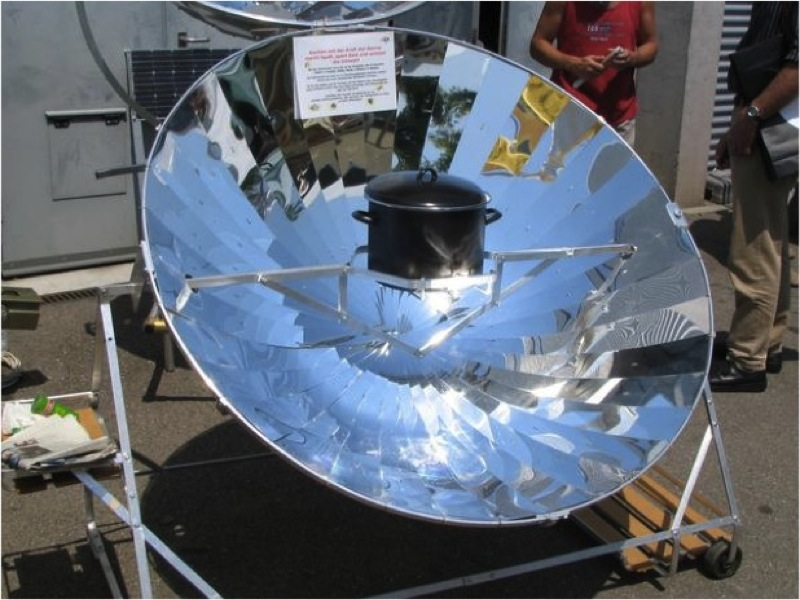
\includegraphics[width=0.382\textwidth]{pictures/herd}
\caption{Kochen}
\end{figure}

\subsection{Mehr Anwendungen}
Folgende Bilder zu Anwendungen von quadratischen Funktionen unter Ausn\"utzung der Parabeleigenschaften.

\begin{figure}
\centering
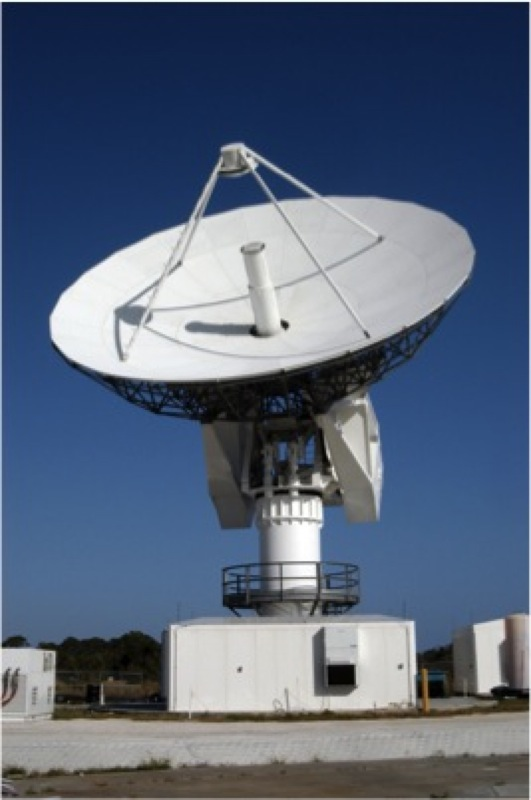
\includegraphics[width=0.3\textwidth]{pictures/radar}
\caption{Signalverst\"arkung}
\end{figure}

\begin{figure}
\centering
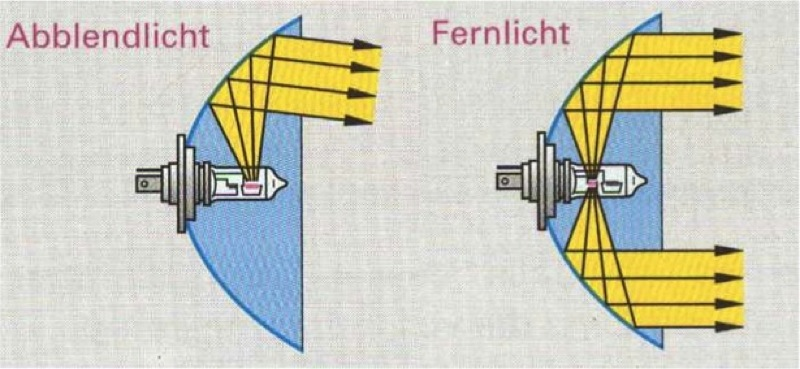
\includegraphics[width=0.5\textwidth]{pictures/scheinwerfer}
\caption{Scheinwerfer}
\end{figure}

\pagebreak

\subsection{Scheitelform}
\begin{wrapfigure}{r}{0.382\textwidth}
  \begin{center}
    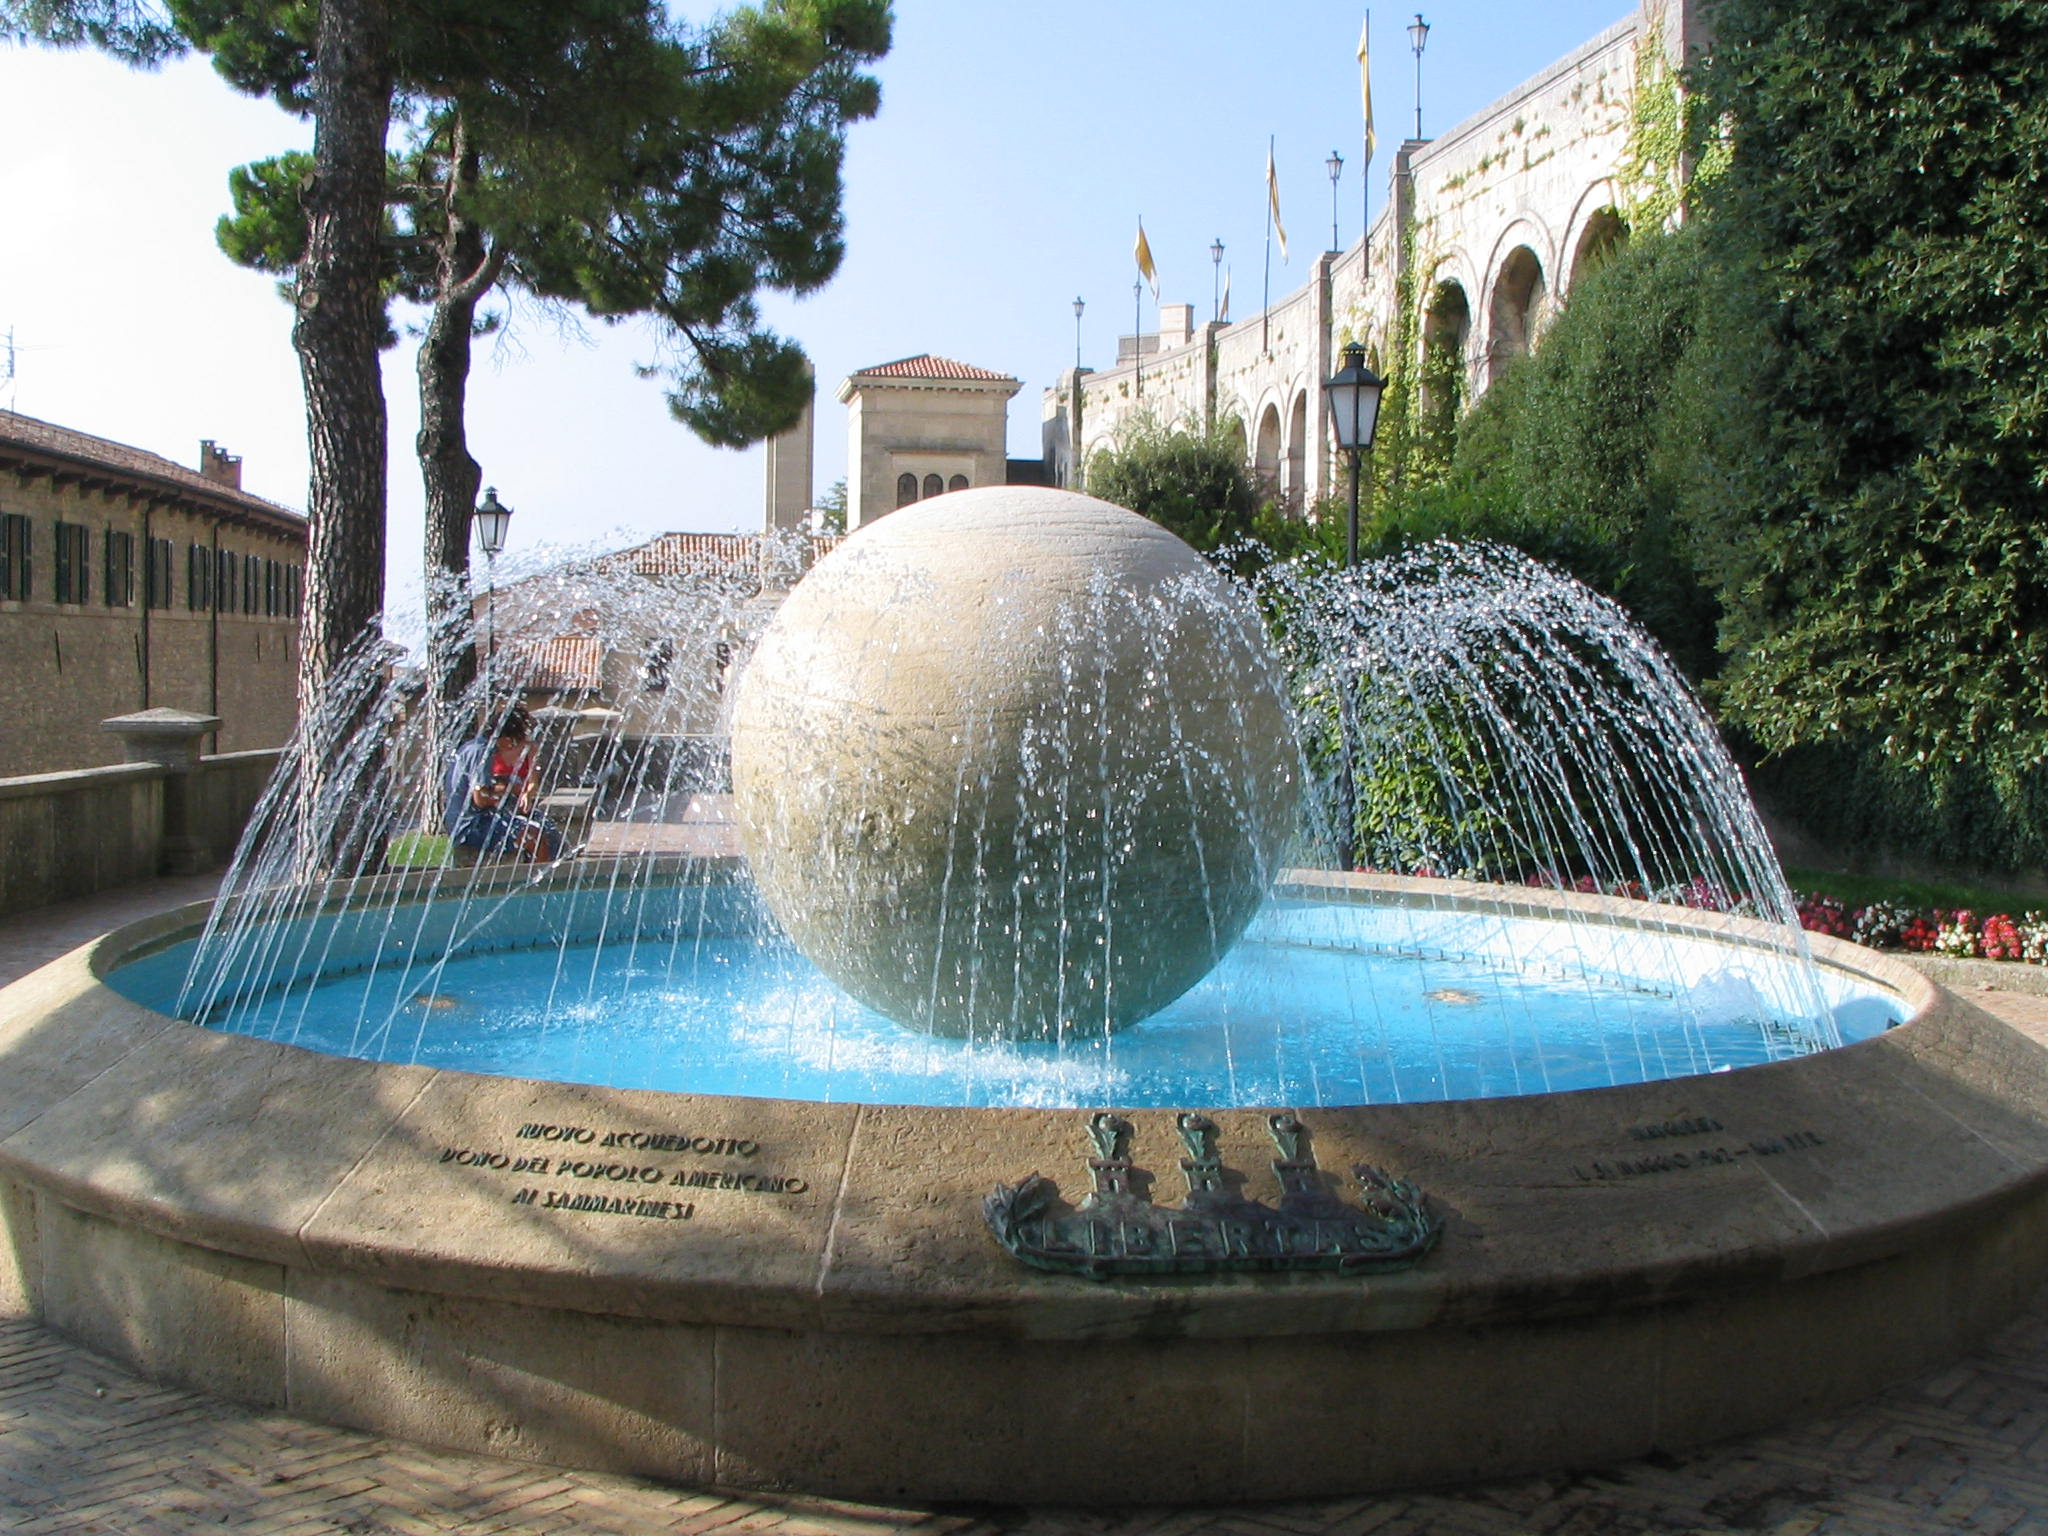
\includegraphics[width=0.382\textwidth]{pictures/springbrunnen}
  \end{center}
%\caption{You Know my Name}
\end{wrapfigure}
Wir haben gesehen, dass der Graph von
$$f(x)=ax^2$$
eine Parabel ist. Die Parabel ist f\"ur $a>0$ nach oben, f\"ur $a<0$ nach unten ge\"offnet. F\"ur $\abs{a}<1$ ist sie weiter, f\"ur $\abs{a}>1$ enger als die Normalparabel. lhr Scheitel ist $S\point{0}{0}$.

Der
\marginnote{
\qrcode{
https://www.youtube.com/watch?v=SD8hHTx36zc}
}
Graph von
$$f(x)=ax^2+v\q(a,v\in\mR)$$
entsteht durch Verschiebung einer Parabel in y-Richtung um $\abs{v}$ Einheiten. F\"ur $v>0$ ist die Parabel nach oben, f\"ur $v<0$ nach unten verschoben. Ihr Scheitel ist $S\point{0}{v}$.

\begin{ueb}[Graphen]
Zeichne in ein und dasselbe Koordinatensystem die Graphen
der Funktionen $f:x\mapsto$
\begin{enumeratea}
\item $(x-2)^2, (x+2)^2, \frac{1}{2}(x-1)^2, -2(x+2)^2$, $x^2+6x+9$
\item $(x-1)^2+1, \frac{1}{2}(x+2)^2-3, -2(x+3)^2+44$, $x^2-3x-2.$
\end{enumeratea}
\end{ueb}

Der Graph von
$$f(x)=a(x-u)^2\q(a,u,\in\mR)$$
entsteht durch Verschiebung einer Parabel in $x$-Richtung um $\abs{u}$ Einheiten. Die Parabel ist f\"ur $u>0$ nach rechts, f\"ur $u<0$ nach links verschoben. Ihr Scheitel ist $S\point{u}{0}$.

Der
\marginnote{
\qrcode{
https://www.youtube.com/watch?v=XcB4ISS-Oso}
}
Graph von
$$f(x)=a(x-u)^2+v\q(a,u,v\in\mR)$$
ist die in x-Richtung um $\abs{u}$ Einheiten und in $y$-Richtung um $\abs{v}$ Einheiten verschobene Parabel mit der Gleichung $y=ax^2$.

\begin{cdef}[Scheitelform]{}
  Da man in dieser Darstellung aus dem Funktionsterm direkt den Scheitel $S\point{u}{v}$ ablesen kann, nennt man
  $$f(x) = a(x - u)^2 + v$$
  Scheitelgleichung oder \emph{Scheitelform} der Parabel.
\end{cdef}

Durch Umformen der Scheitelgleichung erh\"alt man die Normalform $f(x)=ax^2+bx+c$. Umgekehrt kann man $f(x)=ax^2+bx+c$ durch quadratische Erg\"anzung immer in die Scheitelgleichung \"uberf\"uhren.

\begin{bem}\label{parametera}
Beachten Sie, dass der Parameter $a$ bei beiden Formen denselben Wert hat.
\end{bem}

\begin{ueb}[$a$ bleibt $a$]
Zeigen Sie die Aussage aus obiger Bemerkung.
\end{ueb}

\begin{bsp}
Es ist klar, dass man durch Ausmultiplizieren und Zusammenfassen aus der Scheitelform die Form $ax^2+bx+c$ erh\"alt. Wie erh\"alt man umgekehrt die Scheitelform? Sei
$$f(x)=3x^2-30x+37.$$

Wir
\marginnote{
\qrcode{
https://www.youtube.com/watch?v=uZIc9wXmO3c}
}
generieren nun eine Form $(x-u)^2$ und passen $v$ \glqq k\"unstlich\grqq\ an. Man nennt das folgende Vorgehen \emph{quadratische Erg\"anzung:}
\begin{align*}
f(x)&=3x^2-30x+37\\
&=3[(x-5)^2-25]+37\\
&=3(x-5)^2-38
\end{align*}
Der Scheitel ist somit $S\point{5}{-38}$ und der Graph l\"asst sich sofort skizzieren.
\end{bsp}

\begin{cdef}[Polynom 2. Grades]{}
Die Funktion
$$f(x)=ax^2+bx+c \q(a,b,c\in\mR)$$
mit $a\neq0$ heisst \emph{quadratische Funktion}; oder ganzrationales Polynom 2. Grades, falls $a,b,c\in\mQ$.
\end{cdef}

\begin{bem}
Ihr Graph ist eine Parabel; ihre Symmetrieachse ist die Parallele zur $y$-Achse durch den Scheitel $S$. Die Parabel ist f\"ur $a>0$ nach oben, f\"ur $a<0$ nach unten ge\"offnet.
\end{bem}

\begin{ueb}[Scheitelgleichung]
Zeichne
\marginnote{
\qrcode{
https://www.youtube.com/watch?v=1dmXQwTQDT4}
}
in dasselbe Koordinatensystem die Graphen der quadratischen Funktionen $x\mapsto$
\begin{enumeratea}
\item $x^2-6x+11, 2x^2-3x, -x^2+6x-7,$
\item $0.5x^2-4x+7, 0.25x^2-2x+1, -0.1x^2-x-1.$
\end{enumeratea}
Hint: Ermittle die Scheitelgleichung und damit die Koordinaten des Scheitels.
\end{ueb}

\pagebreak

\begin{ueb}[Parabel, ist nicht linear\dots]
Wie lautet die Gleichung der Parabeln?
\begin{center}
\definecolor{cqcqcq}{rgb}{0.75,0.75,0.75}
\begin{tikzpicture}[line cap=round,line join=round,>=triangle 45,x=0.75cm,y=0.75cm]
\draw [color=cqcqcq,dash pattern=on 2pt off 2pt, xstep=0.55cm,ystep=0.55cm] (-4.3,-4.16) grid (7.6,6.3);
\draw[->,color=black] (-4.3,0) -- (8.14,0);
\foreach \x in {-4,-3,-2,-1,1,2,3,4,5,6,7}
\draw[shift={(\x,0)},color=black] (0pt,2pt) -- (0pt,-2pt) node[below] {\footnotesize $\x$};
\draw[->,color=black] (0,-4.16) -- (0,6.3);
\foreach \y in {-4,-3,-2,-1,1,2,3,4,5,6}
\draw[shift={(0,\y)},color=black] (2pt,0pt) -- (-2pt,0pt) node[left] {\footnotesize $\y$};
\draw[color=black] (0pt,-10pt) node[right] {\footnotesize $0$};
\clip(-4.3,-4.16) rectangle (8.14,6.3);
\draw[smooth,samples=100,domain=-4.3:8.14] plot(\x,{2*(\x+2)^2-3});
\draw[smooth,samples=100,domain=-4.3:8.14] plot(\x,{0.5*(\x-4)^2+1});
\draw[smooth,samples=100,domain=-4.3:8.14] plot(\x,{0-(\x-3)^2-1});
\draw[color=black] (-3.8,6) node {$f$};
\draw[color=black] (1.2,6) node {$g$};
\draw[color=black] (1.6,-3.8) node {$h$};
\end{tikzpicture}
\end{center}
\end{ueb}

\begin{ueb}[Gebiete]
Schraffiere in einem Koordinatensystem die Punktmenge
\begin{enumeratea}
\item $\mM=\setm{(x|y)}{y<2-x^2\text{ und }y>2x-x^2}$
\item $\mM=\setm{(x|y)}{y<1-x^2\text{ und }y\geq x-1}$
\item $\mM=\setm{(x|y)}{y\leq2-0.5x^2\text{ und }y>x-2}$
\end{enumeratea}
\end{ueb}

\begin{ueb}[Gleichungen]
Ermittle die Scheitelgleichung der Parabel mit dem Scheitel $S$ so, dass sie durch den Punkt $P$ geht.
\begin{enumeratea}
\item $S\point{2}{4}$, $P\point{3}{3}$
\item $S\point{2}{4}$, $P\point{-1}{7}$
\item $S\point{-2}{-3}$, $P\point{0}{0}$
\end{enumeratea}
\end{ueb}

\begin{ueb}[Parameter hie und da]
Ermittle die Gleichung $y=x^2+bx+c$ einer Parabel so, dass sie durch die Punkte $A\point{2}{-7}$ und $B\point{-3}{8}$ geht.
\end{ueb}

\begin{ueb}[Parameter hie und da und dort]
Ermittle
\marginnote{
\qrcode{
https://www.youtube.com/watch?v=v_QwU5hnazM}
}
die Gleichung $y=ax^2+bx+c$ einer Parabel so, dass sie durch die Punkte $A$, $B$ und $C$ geht.
\begin{enumeratea}
\item $A\point{1}{0}, B\point{-1}{1}$ und $C\point{2}{1}$
\item $A\point{1}{2}$, $B\point{3}{4}$ und $C\point{5}{1}$
\end{enumeratea}
\end{ueb}

\pagebreak

\begin{ueb}[Lastwagen]
Ein
\marginnote{
\qrcode{
https://www.youtube.com/watch?v=FfNwbXLpFwk}
}
Br\"uckenbogen hat die Form einer Parabel. Die Scheitelh\"ohe betr\"agt $\unit[4]{m}$, die Spannweite $\unit[8]{m}$.
\begin{enumeratea}
\item Kann ein Lastwagen mit einer H\"ohe von $\unit[3.5]{m}$ und
einer Breite von $\unit[2.1]{m}$ passieren?
\item Wie breit darf der Lastwagen h\"ochstens sein?
\item Kann der Lastwagen aus (a) zugleich mit einem
Pkw der H\"ohe $\unit[1.6]{m}$ und der Breite $\unit[1.8]{m}$ passieren, wenn zwischen ihnen ein Abstand von $\unit[0.3]{m}$ bleiben soll?
\end{enumeratea}
\end{ueb}

\begin{ueb}[Vinyl]
Die Einnahmen einer Schallplattenfirma in Abh\"angigkeit des Verkaufspreises $x$ (in Fr./Schallplatte) einer Schallplatte k\"onnen durch den Funktionsterm
$$E(x) =600x - 30x^2$$
beschrieben werden. Die Kosten in Abh\"angigkeit des Verkaufspreises pro Platte betragen 
$$K(x) =4320 - 180x.$$
Zeichne in einem geeigneten Koordinatensystem die Graphen der beiden Funktionen $E$ und $K$. In welcher Bandbreite kann der Preis pro Platte liegen, wenn die Firma ohne Verlust arbeiten will? Welchen Preis soll sie festlegen, damit der Gewinn m\"oglichst gross wird? Beantworte die Fragen mit Hilfe der Graphik!
\end{ueb}

\begin{bem}
Die letzte Aufgabe kann auch rechnerisch gel\"ost werden. Der Gewinn $G(x)$ der Firma l\"asst sich n\"amlich mit Hilfe der Funktionen $E$ und $K$ durch den Funktionsterm
\begin{align*}
G(x) &=E(x) - K(x)\\
&=(600x-30x^2) - (4320 - 180x)\\
&=- 30x^2 + 780x - 4320\\
&=750 - 30(x - 13)^2
\end{align*}
beschreiben. Der Graph von G ist eine nach unten ge\"offnete Parabel. Die $x$-Koordinate des Scheitels gibt den Preis pro Platte an, den die Firma verlangen muss, um einen m\"oglichst grossen Gewinn zu erzielen. Die $y$-Koordinate des Scheitels entspricht dem maximalen Gewinn.
\end{bem}

\begin{ueb}[Leistung]
Die Abbildung \ref{abb:dieselmotor} auf Seite \pageref{abb:dieselmotor} zeigt die Kennlinien eines Dieselmotors. Drehmoment, Leistung und Kraftstoffverbrauch (in g Kraftstoff pro kWh) sind als Funktionen der Drehzahl aufgetragen.

\begin{figure}
\begin{center}
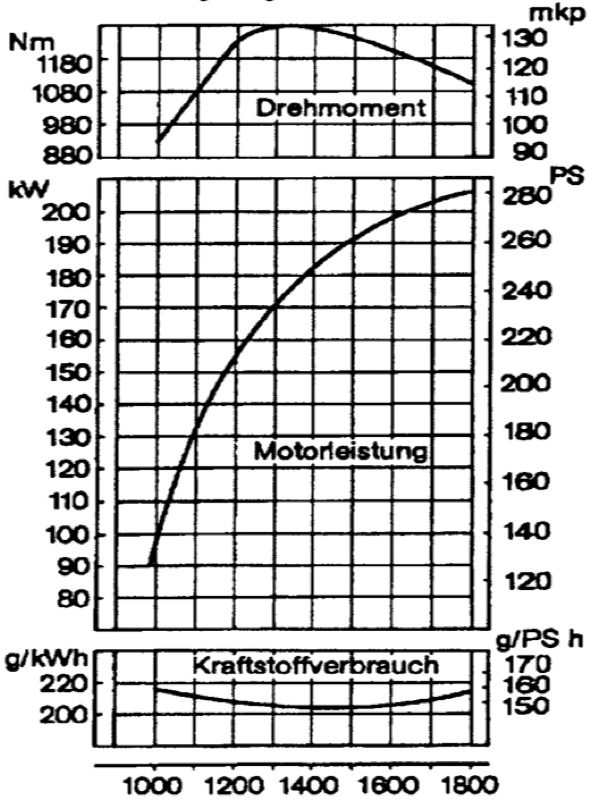
\includegraphics[width=0.5\textwidth,angle=-0.2]{pictures/motor}
\end{center}
\caption{Kennlinien eines Dieselmotors}\label{abb:dieselmotor}
\end{figure}
Welche der drei Kurven kann man durch Parabeln n\"ahern? Stelle die Gleichungen auf und pr\"ufe die G\"ute der N\"aherung durch Berechnung einiger Zwischenwerte.
Hint: W\"ahle bei der Leistung $\point{1000}{70}$ als Ursprung und gib die Koordinaten als Gittereinheiten an. Man erh\"alt die Punkte $\point{0}{2.5}$, $\point{4}{11.2}$, $\point{8}{13.6}$. Beim Kraftstoffverbrauch erh\"alt man mit dem Punkt $\point{1000}{180}$ als Ursprung in Gittereinheiten die Punkte $\point{0}{1.8}$, $\point{4}{1.2}$, $\point{8}{1.7}$.
\end{ueb}

\subsection{Maxima \&\ Minima}
Der gr\"osste bzw. kleinste Wert einer Wertemenge heisst \emph{Maximum} bzw. \emph{Minimum}. Die quadratische Funktion
$$f(x)=ax^2+bx+c=a(x-u)^2+v$$
hat f\"ur
$$x =u=-\frac{b}{2a}$$
ein Maximum, falls $a<0$, bzw. ein Minimum, falls $a>0$. Das Maximum bzw. Minimum ist $v =f(u)$.

Begr\"undung: Der Term $(x - u)^2$ ist nicht negativ; f\"ur $a <0$ wird $f(x)\leq v$ und f\"ur $a > 0$ wird $f(x) \geq v$. Das Gleichheitszeichen gilt aber nur f\"ur $x =u$.

\begin{ueb}[Extremwerte]
Ermittle das Maximum bzw. das Minimum der folgenden Terme f\"ur $x\in\mR$.
$$x^2 -8x + 25, 3 - 2x - x^2, x^2 + x -18, - x^2 + 6x + 2.$$
\end{ueb}

\pagebreak

\begin{ueb}[Maximize]
Welches Rechteck vom Umfang $\unit[160]{cm}$ hat den gr\"ossten Inhalt?
\end{ueb}

\begin{ueb}[Maximize again]
Mit $\unit[120]{m}$ Zaun soll ein m\"oglichst grosses rechteckiges Feld abgegrenzt werden,
\begin{enumeratea}
\item auf offenem Gel\"ande,
\item wenn an einer Seite ein Fluss die Grenze bildet.
\end{enumeratea}
Wie gross wird jeweils das Feld?
\end{ueb}

\begin{ueb}[Maximize once again]
Ein Jazzlokal hat bei einem Eintritt von $\unit[8]{Fr.}$ durchschnittlich 240 Besucher. W\"urde man den Eintrittspreis um $\unit[0.5]{Fr.}$, $\unit[1]{Fr.}$ usw. erh\"ohen, so ginge die Besucherzahl um 10, 20 usw. zur\"uck. Bei welchem Eintrittspreis sind die Einnahmen am gr\"ossten?
\end{ueb}

\begin{ueb}[Turbine]
Die Leistung einer Turbine h\"angt von der Drehzahl $n$ ab. Die Gleichung
$$L = 300n - 0.8n^2$$
gibt die Leistung einer Turbine in Watt an. Bei welcher Drehzahl hat diese Turbine die gr\"osste Leistung? Wie hoch ist diese?
\end{ueb}

\begin{ueb}[Lampe]
Der Schirm einer Stehlampe soll die Form einer quadratischen S\"aule haben. F\"ur das Gestell stehen $\unit[440]{cm}$ Draht zur Verf\"ugung.
\begin{enumeratea}
\item Welche Ausmasse hat der Lampenschirm, wenn
der Mantel zur dekorativen Gestaltung m\"oglichst
gross sein soll? Wie gross ist diese Mantelfl\"ache?
\item Wie sind die Ergebnisse, wenn f\"ur eine entsprechende H\"angelampe die Oberfl\"ache maximal sein
soll?
\end{enumeratea}
\end{ueb}

\subsection{Rechnerische L\"osung von quadratischen Gleichungen}
\subsubsection{Die reinquadratische Gleichung}
\begin{cdef}[Reinquadratische Gleichung]{}
  Eine \emph{reinquadratische Gleichung} ist eine Gleichung der Form
  $$x^2-c=0$$ wobei $c\in\D{R}$.
\end{cdef}
\begin{csatz}[Lösung der reinquadratischen Gleichung]{}
  Die reinquadratische Gleichung hat f\"ur $c<0$ keine L\"osung, f\"ur $c=0$
  die L\"osung $x=0$ und f\"ur $c>0$ die L\"osungen
  $$x_1=\sqrt{c}\quad\text{und}\quad x_2=-\sqrt{c}$$
\end{csatz}
\begin{bew}
  Einsetz\"ubung.
\end{bew}

\subsubsection{Die allgemeine quadratische Gleichung}
\begin{cdef}[Quadratische Gleichung]{}
  Eine
  \marginnote{
\qrcode{
https://www.youtube.com/watch?v=MWVyS0jIL98}
}
  Gleichung heisst \emph{quadratisch}, wenn sie sich in der
  Form
  $$ax^2+bx+c=0$$ schreiben l\"asst, wobei $a,b,c\in\D{R}$ und
  $a\neq0$ ist.
\end{cdef}
\begin{csatz}[Lösungsformel der quadratischen Gleichung]{}
  Die
    \marginnote{
\qrcode{
https://www.youtube.com/watch?v=HdHpXhDCBL0}
}
  quadratische Gleichung $ax^2+bx+c=0$ hat die L\"osungen
  $$x_{1,2}=\frac{-b\pm\sqrt{b^2-4ac}}{2a}$$ Die Anzahl der L\"osungen
  h\"angt vom Term unter der Wurzel ab.
\end{csatz}
\begin{bew}
  Quadratische Erg\"anzung.
\end{bew}

\begin{cdef}[Diskriminante]{}
  Der Term unter der Wurzel, $D=b^2-4ac$, heisst
  \emph{Diskriminante}.
\end{cdef}

\begin{csatz}[Anzahl Lösungen einer quadratischen Gleichung]{}
  Die quadratische Gleichung $ax^2+bx+c=0$ hat
  \begin{itemize}
    \item zwei L\"osungen, falls $b^2-4ac>0$
    \item eine L\"osung, falls $b^2-4ac=0$
    \item keine L\"osung, falls $b^2-4ac<0$
  \end{itemize}
\end{csatz}
\begin{bew}
  Nach Definition der Wurzel.
\end{bew}

\begin{ueb}
  Gib je ein Beispiel einer reinquadratischen Gleichung die
  keine L\"osung bzw. zwei L\"osungen hat.
\end{ueb}

\begin{ueb}
  Bringe die Gleichung $$7x^2=-(33x+36)$$ in die Form
  $ax^2+bx+c=0$, und bestimme die Koeffizienten $a$, $b$ und
  $c$.
\end{ueb}

\begin{ueb}
  Bestimme die L\"osungsmenge der Gleichung
  $$7x^2+33x+36=0$$
\end{ueb}

\begin{ueb}
  Bestimme die L\"osungsmenge der Gleichung
  $$80x^2-166x+51=0$$
\end{ueb}

\begin{ueb}
  Bestimme die L\"osungsmenge der Gleichung
  $$x^2-2x+1=0$$
\end{ueb}

\begin{ueb}
  Bestimme die L\"osungsmenge der Gleichung
  $$3x^2-2x+1=0$$
\end{ueb}

\begin{ueb}
  Bestimme die L\"osungsmenge der Gleichung
  $$x^2+2ex-3e^2=0$$
\end{ueb}

\begin{ueb}
  Bestimme die L\"osungsmenge der Gleichung
  $$x^2-4x+3+2a-a^2=0$$
\end{ueb}

\subsubsection{Beziehungen zwischen Koeffizienten und L\"osungen einer
quadratischen Gleichung}
\begin{csatz}[von Viëta]{}
  Sind $x_1$ und $x_2$ L\"osungen der Gleichung
  $x^2+px+q=0$, so gilt:
  $$x_1+x_2=-p\quad\text{und}\quad x_1\cdot x_2=q$$
\end{csatz}

\begin{bew}
  \"Ubung
\end{bew}

\pagebreak

\begin{csatz}[Linearfaktor-Zerlegung]{}
  Sind $x_1$ und $x_2$ die L\"osungen der Gleichung $x^2+px+q=0$ so
  l\"asst sich diese stets in Linearfaktoren zerlegen:
  $$(x-x_1)(x-x_2)=0$$
\end{csatz}

\begin{bem}
  Dieser Satz eignet sich vor allem zum Kreieren von quadratischen
  Gleichungen mit vorgegebener L\"osung und zum L\"osen von
  quadratischen Gleichungen mit ganzzahligen L\"osungen.
\end{bem}

\begin{ueb}
  L\"ose mit Zerlegung in Linearfaktoren:\\[2ex]
  \begin{minipage}{0.49\textwidth}
    \begin{enumeratea}
      \item $x^2-8x+15=0$
      \item $x^2+9x+18=0$\\[1ex]
    \end{enumeratea}
  \end{minipage}
  \begin{minipage}{0.49\textwidth}
    \begin{enumeratea}\addtocounter{enumi}{2}
      \item $18x^2-9x+1=0$
      \item $x^2-(a+b)x+ab=0$\\[1ex]
    \end{enumeratea}
  \end{minipage}
\end{ueb}

\begin{ueb}
  Gib eine quadratische Gleichung an, die folgende L\"osung hat:\\[2ex]
  \begin{minipage}{0.49\textwidth}
    \begin{enumeratea}
      \item $x_1=2$ und $x_2=3$.
    \end{enumeratea}
  \end{minipage}
  \begin{minipage}{0.49\textwidth}
    \begin{enumeratea}\addtocounter{enumi}{1}
      \item $x_1=\frac{1}{2}$ und $x_2=\pi$.
    \end{enumeratea}
  \end{minipage}
\end{ueb}

\clearpage

\section{Trigonometrische Funktionen}

\subsection{Die Sinusfunktion}

\begin{erin}
Ein rechtwinkliges Dreieck ist bestimmt durch zwei Seiten oder eine Seite und einen spitzen Winkel. Gleichschenklige Dreiecke, Rechtecke etc. lassen sich auf rechtwinklige Dreiecke zurückführen.
\end{erin}

\begin{ueb}[Sinus]
  Zeichne zwei rechtwinklige Dreiecke, bei denen ein spitzer
  Winkel $35^\circ$ beträgt. Bestimme bei beiden Dreiecken das
  Verhältnis
  $$\frac{\text{Gegenkathete des $35^\circ$
  Winkels}}{\text{Hypotenuse}} = \frac{g}{h}$$
  Als \emph{Gegenkathete} bezeichnet man diejenige Kathete, welche dem gegebenen Winkel gegenüber liegt.
\end{ueb}
Weil die beiden Dreiecke ähnlich sind, sind die berechneten
Verhältnisse theoretisch gleich gross; und zwar für sämtliche rechtwinkligen
Dreiecke mit dem Winkel $35^\circ$. Deshalb hat man festgelegt:
\begin{cdef}[Sinus]{}
  In
  \marginnote{
\qrcode{
https://www.youtube.com/watch?v=SuihLS5YEOI}
}
  einem rechtwinkligen Dreieck heisst das Verhältnis von
  Gegenkathete zu Hypotenuse \emph{Sinus} des der Kathete
  gegenüberligenden Winkels, und man schreibt
  $$\sin(\alpha) = \frac{\text{Gegenkathete}}{\text{Hypotenuse}} =
  \frac{g}{h}$$
\end{cdef}

\begin{figure}
\begin{center}
\definecolor{qqttzz}{rgb}{0,0.2,0.6}
\definecolor{qqwuqq}{rgb}{0,0.39,0}
\definecolor{qqqqff}{rgb}{0,0,1}
\scalebox{1}{
\begin{tikzpicture}[line cap=round,line join=round,>=triangle 45,x=0.6cm,y=0.6cm]
\clip(0.2,-2.56) rectangle (11.16,3.84);
\draw [shift={(7.06,2.64)},color=qqwuqq] (0,0) -- (-146.01:0.6) arc (-146.01:-56.01:0.6) -- cycle;
\draw [shift={(0.98,-1.46)},line width=1.2pt,color=qqwuqq,fill=qqwuqq,fill opacity=0.1] (0,0) -- (-1.05:1.6) arc (-1.05:33.99:1.6) -- cycle;
\fill[color=qqwuqq] (6.99,2.29) circle (0.02);
\draw [line width=1.6pt] (0.98,-1.46)-- (7.06,2.64);
\draw [line width=1.6pt] (0.98,-1.46)-- (9.93,-1.62);
\draw [line width=1.6pt] (9.93,-1.62)-- (7.06,2.64);
\draw (5.3,-1.6) node[anchor=north west] {$h$};
\draw (3.84,1.4) node[anchor=north west] {$a$};
\draw (8.7,1.2) node[anchor=north west] {$g$};
\draw (1.7,-0.8) node[anchor=north west] {$\alpha$};
\fill [color=qqqqff] (0.98,-1.46) circle (1.5pt);
\draw[color=qqqqff] (0.4,-1.4) node {$A$};
\fill [color=qqqqff] (7.06,2.64) circle (1.5pt);
\draw[color=qqqqff] (7.2,3.2) node {$B$};
\fill [color=qqttzz] (9.93,-1.62) circle (1.5pt);
\draw[color=qqttzz] (10.5,-1.5) node {$C$};
\end{tikzpicture}
}
\end{center}
\caption{Definition der Winkelfunktionen}
\end{figure}

\begin{bem}
Für die Bezeichnungen im rechtwinkligen Dreieck wählt man passend $h$ für die Hypotenuse, $a$ für die Ankathete und $g$ für die Gegenkathete.
\end{bem}

\begin{ueb}[Sin-Taste]
  Berechne mit dem TR $\sin(35^\circ)$.
\end{ueb}
\begin{ueb}[Graph Sin]
  Zeichne
\marginnote{
\qrcode{
https://www.youtube.com/watch?v=wYFdYuesvp4}
}
  den Graphen der Sinusfunktion $f(x)=\sin(x)$ im Intervall $[0^\circ,90^\circ]$. Berechne dazu mit dem Taschenrechner die entsprechenden Funktionswerte. (Wähle Winkel, deren Sinus du exakt bestimmen kannst.)
\end{ueb}
\begin{ueb}[Gugel-Hopf]
  In einem rechtwinkligen Dreieck beträgt die Hypotenuse
  $\unit[12]{cm}$ und ein spitzer Winkel $25^\circ$. Wie lang sind die
  Katheten?
\end{ueb}
\begin{ueb}[Sonnenkollektor]
  Ein rechteckiger Sonnenkollektor der Länge $\unit[2]{m}$ soll
  mit einem Neigungswinkel von $75^\circ$ gegenüber der Horizontalen so
  an eine Hauswand gestellt werden, dass die eine Breite die Wand
  und die andere den Boden berührt. In welcher Höhe über dem Boden
  berührt die eine Breite die Hauswand?
\end{ueb}
\begin{ueb}[Wetterballon]
  Ein kugelförmiger Wetterballon mit Durchmesser $d = \unit[16]{m}$ wird unter einem Sehwinkel $\alpha
  = 22'$ beobachtet. Wie weit ist der Ballon vom Beobachter
  entfernt?
\end{ueb}

\subsection{Die Cosinusfunktion}
\begin{cdef}[Cosinus]{}
  In allen rechtwinkligen Dreiecken mit einem spitzen Winkel
  $\alpha$ ist das Verhältnis von Ankathete von $\alpha$ zu
  Hypotenuse aus Gründen der Ähnlichkeit gleich gross. Man nennt es
  \emph{Cosinus} des der Kathete anliegenden Winkels.
  $$\cos(\alpha) = \frac{\text{Ankathete}}{\text{Hypotenuse}} =
  \frac{a}{h}$$
\end{cdef}

\begin{ueb}[aha]
  Zeichne ein Bild zur Cosinus-Definition.
\end{ueb}
\begin{ueb}[Graph Cos]
  Zeichne den Graphen der Funktion
  $$f(x)=\cos(x)$$
  auf dem Intervall $[0^\circ,90^\circ]$.
\end{ueb}
\begin{ueb}[Leiter]
  Eine Leiter mit der Länge $l = \unit[6.4]{m}$ lehnt an einer Wand.
  Ihr Fuss ist $a = \unit[2.8]{m}$ von der Wand entfernt. Wie gross
  ist ihr Neigungswinkel?
\end{ueb}
\begin{bem}
  Den Winkel in obiger Aufgabe bestimmt man mit der Inversfunktion
  des Cosinus, $\cos^{-1}$ oder auch arccos (sprich \glqq Arcus-Cosinus\grqq) genannt, indem man sie auf beide Seiten der
  Gleichung anwendet:
  \begin{align}
    \cos(\alpha) &= \frac{2.8}{6.4} \tag{$\cos^{-1}$}\\
    \cos^{-1}(\cos(\alpha)) &=
    \cos^{-1}\left(\frac{2.8}{6.4}\right) \notag\\
    \alpha &= \cos^{-1}\left(\frac{2.8}{6.4}\right) \approx 64.1^\circ\notag
  \end{align}
\end{bem}

\begin{bem}
Wie üblich bei Funktionen steht das \glqq$^{-1}$\grqq\ nicht für den Kehrwert, sondern für Inversfunktion von $f$.
\end{bem}

\begin{ueb}[Bahnstrecke]
  Eine Bahnstrecke hat auf der Karte $1\div25\,000$ eine
  Länge von $s = \unit[18]{mm}$ und fällt unter $\alpha = 8^\circ$. Wie
  lang ist sie?
\end{ueb}
\begin{ueb}[Erdrotation]
  Mit
\marginnote{
\qrcode{
https://youtu.be/sBMuUgbNDXM}
}
  welcher Geschwindigkeit bewegen wir uns aufgrund der
  Erdrotation? Überlege dir zuerst anhand einer Skizze, welche Daten du zur Beantwortung der Frage benötigst, und beschaffe diese, um die Geschwindigkeit konkret zu berechnen.
\end{ueb}

\subsection{Die Tangensfunktion}
\begin{cdef}[Tangens]{}
  Im rechtwinkligen Dreieck bezeichnet man das Verhältnis der
  Gegenkathete eines spitzen Winkels $\ga$ zur Ankathete als den
  \emph{Tangens} des Winkels $\ga$.
  $$\tan\ga = \frac{\text{Gegenkathete}}{\text{Ankathete}}=\frac{g}{a}$$
\end{cdef}

\begin{ueb}[geht auch]
  Zeichne ein Bild zur Tangens-Definition.
\end{ueb}
\begin{ueb}[Graph Tan]
  Zeichne den Graphen der Tangensfunktion
  $$f(x)=\tan(x)$$
  über dem Intervall $[0^\circ,90^\circ]$.
\end{ueb}
\begin{ueb}[Tanne]
  Wie hoch ist eine Tanne, wenn ihr Schatten $s = \unit[27.5]{m}$
  lang ist und die Sonnenstrahlen unter dem Winkel $\ga = 38^\circ50'$
  einfallen?
\end{ueb}
\begin{ueb}[Münster]
  Unter welchem Erhebungswinkel erscheint die Spitze des Berner
  Münsters ($h = \unit[161]{m}$) von einer Stelle aus, die in
  waagrechter Richtung $e = \unit[150]{m}$ vom Fuss des Turmes
  entfernt ist? (Augenhöhe $a = \unit[1.5]{m}$)
\end{ueb}
\begin{ueb}[Walmdach]
  Ein
  \marginnote{
    \qrcode{
    https://www.youtube.com/watch?v=Cz6GRngrQcQ}
    }
  Walmdach ist $a = \unit[12]{m}$ lang, $b = \unit[8.8]{m}$
  breit und $h = \unit[4.8]{m}$ hoch. Die Firstlänge beträgt $l =
  \unit[5.4]{m}$. Bestimme durch Zeichung und Rechnung den
  Neigungswinkel der Dachflächen und der Grate.
\end{ueb}

\begin{bem}
Um sich die Definitionen der drei Winkelfunktionen $\sin$, $\cos$ und $\tan$ zu verinnerlichen, gibt es zahlreiche Eselsbrücken.
\end{bem}

\subsection{Das Bogenmass}
Um die Graphen der Sinus- und Cosinus-Funktion zu zeichnen verwendet
man üb\-li\-cher\-wei\-se das sogenannte Bogenmass.
\begin{cdef}[Bogenmass]{}
  Unter
    \marginnote{
\qrcode{
https://www.youtube.com/watch?v=JPsDuUSnjq4}
}
  dem \emph{Bogenmass} $\arc
  \alpha$ des Winkels $\alpha$
  versteht man den Quotienten
  $$\arc\alpha = \frac{b}{r}.$$
  Die \glqq Einheit\grqq\ des Bogenmasses heisst Radian, $\unit{rad}$.

\end{cdef}

\begin{bem}
  Aus Ähnlichkeitsgründen ist das Bogenmass unabhängig von der Wahl
  des Kreisradius.
\end{bem}
Das Bogenmass gibt uns also die Möglichkeit, Winkel als
dimensionslose Zahlenwerte darzustellen. Da das Bogenmass unabhängig
von der Wahl des Kreisradius ist, denke ich mir jeweils einfach für
einen gegebenen Winkel das Bogenmass als Länge des entsprechenden
Kreisbogens im Einheitskreis. Weil dort $r = 1$ ist, vereinfacht
sich das Bogenmass nämlich zu
$$\arc\alpha =\frac{b}{1}=b.$$
Für das Bogenmass in
einem beliebigen Kreis gilt
\begin{csatz}[Bogenlänge]{}
  $$b = r\cdot\arc\alpha$$
\end{csatz}
\begin{proof}[Beweis]
  Folgt direkt aus der Definition.
\end{proof}
\begin{ueb}[Rad]
  Erstelle eine Tabelle für das Bogenmass zu den folgenden
  Winkel im Gradmass: $360^\circ$, $180^\circ$, $90^\circ$, $45^\circ$, $1^\circ$, $\alpha$.
\end{ueb}
Der folgende Satz gibt das Rezept an, wie man zu einem Winkel
$\alpha$ im Gradmass das zugehörige Bogenmass $\arc\alpha$ bestimmt.
\begin{csatz}[Grad in Radian]{}
  $$\arc\alpha = \frac{\pi\cdot\alpha}{180^\circ}$$
\end{csatz}
\begin{proof}[Beweis]
  Es gilt $$\arc\alpha = \frac{b}{r}$$ wobei die Länge des Bogens
  $b$ abhängig vom Winkel $\alpha$ ist und den Bruchteil $\frac{\alpha}{360^\circ}$
  des ganzen Kreisumfangs $2\pi r$ ausmacht. Also
  $$\arc\alpha = \frac{2\pi r\cdot\frac{\alpha}{360^\circ}}{r} =
  \frac{2\pi\cdot\alpha}{360^\circ}= \frac{\pi\cdot\alpha}{180^\circ}$$
\end{proof}
\begin{bem}
  Der Taschenrechner kann Winkel unter anderem im Bogen- oder
  Gradmass darstellen. Setzt man im \fbox{Mode} die Variable Angle auf \glqq Rad\grqq, so
  interpretiert er Winkel im Bogenmass (Radian), wählt man \glqq Deg\grqq, so
  erwartet er Winkel im Gradmass (Degree).
\end{bem}
\begin{ueb}[TR-Mode]
  Zeichne die Graphen der Sinus- und Cosinus-Funktion. Wähle auf der $x$-Achse die Winkel im Bogenmass.
\end{ueb}
Aus der vorigen Aufgabe lässt sich folgender Satz ablesen:
\begin{csatz}[Sinus-Cosinus-Beziehung]{}
  Die Graphen der Sinus- und Cosinus-Funktion sind zueinander
  achsialsymmetrisch bezüglich der Parallelen zur $y$-Achse durch den
  Punkt $\point{\frac{\pi}{4}}{0}$.
\end{csatz}
Es gibt offenbar zu jedem Sinus-Wert einen gleich grossen
Cosinus-Wert und umgekehrt. Diese Tatsache lässt sich durch folgende
Formel ausdrücken:
  \begin{align}
    \sin(\alpha) &= \cos(90^\circ - \alpha) \notag\\
    \cos(\alpha) &= \sin(90^\circ + \alpha) \notag
  \end{align}
\begin{proof}[Beweis der beiden vorherigen Sätze]
  Nach Definition
\end{proof}
Wir wollen die beiden eben kennengelernten Winkelfunktionen betrachten und stellen sie als Funktion in Abhängigkeit des Winkels dar. Dabei kann man in natürlicher Weise die Funktionen für beliebige Winkel definieren. Die
    \marginnote{
\qrcode{
https://www.youtube.com/watch?v=EbaADp9boU0}
}
Graphen von 
$$f(\alpha)=\sin(\ga)$$
und 
$$g(\ga)=\cos(\ga)$$
sehen wie folgt aus:

\begin{figure}
\centering
\definecolor{cqcqcq}{rgb}{0.75,0.75,0.75}
\scalebox{1}{
\begin{tikzpicture}[line cap=round,line join=round,>=triangle 45,x=0.5cm,y=1.25cm]
\draw [color=cqcqcq,dash pattern=on 2pt off 2pt, xstep=0.785cm,ystep=0.625cm] (-7.5,-2) grid (7.5,2);
\draw[->,color=black] (-7.5,0) -- (7.5,0);
\foreach \x in {-2,-1.5,-1,-0.5,0.5,1,1.5,2}
\draw[shift={(3.14*\x,0)},color=black] (0pt,2pt) -- (0pt,-2pt) node[below] {\footnotesize $\x\pi$};
\draw[color=black] (7.16,0.03) node [anchor=south west] { x};
\draw[->,color=black] (0,-2) -- (0,2);
\foreach \y in {-2,-1.5,-1,-0.5,0.5,1,1.5}
\draw[shift={(0,\y)},color=black] (2pt,0pt) -- (-2pt,0pt) node[left] {\footnotesize $\y$};
\draw[color=black] (0.1,1.85) node [anchor=west] { y};
\draw[color=black] (0pt,-10pt) node[right] {\footnotesize $0$};
\clip(-7.5,-2) rectangle (7.5,2);
\draw[line width=1.6pt, smooth,samples=100,domain=-7.5:7.5] plot(\x,{sin(180/3.14*\x)});
\end{tikzpicture}
}
\caption{Graph von $\sin(x)$}
  \end{figure}
  
\begin{figure}
\centering
\definecolor{cqcqcq}{rgb}{0.75,0.75,0.75}
\scalebox{1}{
\begin{tikzpicture}[line cap=round,line join=round,>=triangle 45,x=0.5cm,y=1.25cm]
\draw [color=cqcqcq,dash pattern=on 2pt off 2pt, xstep=0.785cm,ystep=0.625cm] (-7.5,-2) grid (7.5,2);
\draw[->,color=black] (-7.5,0) -- (7.5,0);
\foreach \x in {-2,-1.5,-1,-0.5,0.5,1,1.5,2}
\draw[shift={(3.14*\x,0)},color=black] (0pt,2pt) -- (0pt,-2pt) node[below] {\footnotesize $\x\pi$};
\draw[color=black] (7.16,0.03) node [anchor=south west] { x};
\draw[->,color=black] (0,-2) -- (0,2);
\foreach \y in {-2,-1.5,-1,-0.5,0.5,1,1.5}
\draw[shift={(0,\y)},color=black] (2pt,0pt) -- (-2pt,0pt) node[left] {\footnotesize $\y$};
\draw[color=black] (0.1,1.85) node [anchor=west] { y};
\draw[color=black] (0pt,-10pt) node[right] {\footnotesize $0$};
\clip(-7.5,-2) rectangle (7.5,2);
\draw[line width=1.6pt, smooth,samples=100,domain=-7.5:7.5] plot(\x,{cos(180/3.14*\x)});
\end{tikzpicture}
}
  \caption{Graph von $\cos(x)$}
  \end{figure}
  
\definecolor{ttwwqq}{HTML}{84B7E1}
\definecolor{ccqqtt}{HTML}{57C286}
\definecolor{cqcqcq}{HTML}{E26A6A}

\begin{figure}
\centering

\begin{tikzpicture}[line cap=round,line join=round,>=triangle 45,x=1.8cm,y=1.8cm]

\draw [color=lightgray,dash pattern=on 2pt off 2pt, xstep=2.826cm,ystep=1.8cm] (-6.5,-3) grid (6.5,3);
\draw[->,color=black] (-6.5,0) -- (6.5,0);
\foreach \x in {-2,-1.5,-1,-0.5,0.5,1,1.5,2}
\draw[shift={(3.14*\x,0)},color=black] (0pt,2pt) -- (0pt,-2pt) node[below] {\footnotesize $\x\pi$};
\draw[color=black] (6.5,0.05) node [anchor=south west] {$x$};
\draw[->,color=black] (0,-3) -- (0,3);
\foreach \y in {-3,-2,-1,1,2}
\draw[shift={(0,\y)},color=black] (2pt,0pt) -- (-2pt,0pt) node[left] {\footnotesize $\y$};
\draw[color=black] (0.07,2.76) node [anchor=west] {$y$};
\draw[color=black] (0pt,-10pt) node[right] {\footnotesize $0$};
\clip(-6.5,-3) rectangle (6.5,3);
\draw[line width=1.6pt, smooth,samples=100,domain=-6.5:6.5, color=cqcqcq] plot(\x,{sin(180/3.14*\x)});
\draw[line width=1.6pt,color=ccqqtt, smooth,samples=100,domain=-6.5:6.5] plot(\x,{cos(180/3.14*\x)});
\draw[line width=1.1pt,color=ttwwqq, smooth,samples=100,domain=-1.5:1.5]  plot(\x,{sin(180/3.14*\x)/cos(180/3.14*\x)});
\draw[line width=1.1pt,color=ttwwqq, smooth,samples=100,domain=1.6:4.5]  plot(\x,{sin(180/3.14*\x)/cos(180/3.14*\x)});
\draw[line width=1.1pt,color=ttwwqq, smooth,samples=100,domain=4.9:6.3]  plot(\x,{sin(180/3.14*\x)/cos(180/3.14*\x)});
\draw[line width=1.1pt,color=ttwwqq, smooth,samples=100,domain=-4.5:-1.6]  plot(\x,{sin(180/3.14*\x)/cos(180/3.14*\x)});
\draw[line width=1.1pt,color=ttwwqq, smooth,samples=100,domain=-6.3:-4.9]  plot(\x,{sin(180/3.14*\x)/cos(180/3.14*\x)});
\draw[color=cqcqcq] (-5.8,2.7) node {$\sin(x)$};
\draw[color=ccqqtt] (-5.8,2.2) node {$\cos(x)$};
\draw[color=ttwwqq] (-5.8,1.7) node {$\tan(x)$};
\end{tikzpicture}
\caption{Graphen der Winkelfunktionen}
\end{figure}

\subsection{Zusammenhänge zwischen Sinus, Cosinus und Tangens}
Wir betrachten ein rechtwinkliges Dreieck mit Hypotenuse $h$.

\begin{figure}
\begin{center}
\scalebox{1}{
\definecolor{qqttzz}{rgb}{0,0.2,0.6}
\definecolor{qqwuqq}{rgb}{0,0.39,0}
\definecolor{qqqqff}{rgb}{0,0,1}
\begin{tikzpicture}[line cap=round,line join=round,>=triangle 45,x=0.7cm,y=0.7cm]
\clip(0.2,-2.56) rectangle (12.16,3.84);
\draw [shift={(7.06,2.64)},color=qqwuqq] (0,0) -- (-146.01:0.6) arc (-146.01:-56.01:0.6) -- cycle;
\draw [shift={(0.98,-1.46)},line width=1.2pt,color=qqwuqq,fill=qqwuqq,fill opacity=0.1] (0,0) -- (-1.05:1.6) arc (-1.05:33.99:1.6) -- cycle;
\fill[color=qqwuqq] (6.99,2.29) circle (0.02);
\draw [line width=1.6pt] (0.98,-1.46)-- (7.06,2.64);
\draw [line width=1.6pt] (0.98,-1.46)-- (9.93,-1.62);
\draw [line width=1.6pt] (9.93,-1.62)-- (7.06,2.64);
\draw (5.3,-1.6) node[anchor=north west] {$h$};
\draw (0.5,1.4) node[anchor=north west] {$h\cdot\cos(\alpha)=a$};
\draw (8.2,1.8) node[anchor=north west] {$g=h\cdot\sin(\ga)$};
\draw (1.8,-0.9) node[anchor=north west] {$\alpha$};
\fill [color=qqqqff] (0.98,-1.46) circle (1.5pt);
\draw[color=qqqqff] (0.6,-1.4) node {$A$};
\fill [color=qqqqff] (7.06,2.64) circle (1.5pt);
\draw[color=qqqqff] (7.2,3) node {$B$};
\fill [color=qqqqff] (9.93,-1.62) circle (1.5pt);
\draw[color=qqqqff] (10.3,-1.6) node {$C$};
\end{tikzpicture}
}
\end{center}
\end{figure}

\noindent Aus der Figur erkennt man:

\newpage

\begin{csatz}[Beziehungen zwischen den Winkelfunktionen]{satz:sincos}\label{satz:sincos}
  \begin{align}
    &\sin^2(\ga) + \cos^2(\ga) = 1\\[1ex]
    &\tan(\ga) = \frac{\sin(\ga)}{\cos(\ga)}
  \end{align}
\end{csatz}

\begin{proof}[Beweis]
Übung
\end{proof}

\begin{bem}
  Anstelle von $(\sin(\ga))^2$ schreibt man kürzer $\sin^2(\ga)$ (sprich:\glqq
  Sinusquadrat Alpha\grqq); dito für die anderen Winkelfunktionen.
\end{bem}
\begin{bem}
Hat man die Sinus-Werte beliebiger Winkel, so lassen sich daraus
auch die Cosinus- und Tangens-Werte berechnen. Man benutzt dazu den
obigen Satz.
\end{bem}

\begin{ueb}[Kopfrechnen]
  Es sei $\sin(\ga) = 0.6$. Berechne mit Hilfe der Formeln aus Satz \ref{satz:sincos} $\cos(\ga)$ und $\tan(\ga)$. (ohne TR)
\end{ueb}

\begin{ueb}[exakt]\label{sinwert}
  Berechne die Werte der trigonometrischen Funktionen für die
  Winkel $30^\circ$, $45^\circ$ und $60^\circ$ mit Hilfe der Definitionen. Gib die Werte als Brüche an. (ohne TR)
\end{ueb}

\begin{bem}
Auf diese Weise lassen sich die trigonometrischen Funktionswerte nur
für spe\-ziel\-le Winkel berechnen. Zur Berechnung der Sinus-Werte
beliebiger Winkel, kann man folgende Formel verwenden, die wir
später herleiten werden (im SF AM):
$$\sin(x) = x-\frac{x^3}{3!}+\frac{x^5}{5!}-\frac{x^7}{7!}+\dots$$
\end{bem}
\begin{bem}
\
  \begin{itemize}
    \item $n!$ bedeutet $1\cdot2\cdot3\cdot\dots\cdot n$, sprich
    \glqq $n$ Fakultät\grqq.
    \item Die Formel gilt nur, wenn $x$ im Bogenmass angegeben wird.
  \end{itemize}
\end{bem}
\begin{ueb}[Sin-Reihe]
  Berechne mit der oben angegebenen Formel $\sin(45^\circ)$
  nä\-he\-rungs\-wei\-se mit den ersten vier Summanden, und vergleiche
  das Resultat mit dem Wert aus Übung \ref{sinwert}.
\end{ueb}

\begin{ueb}[umschreiben]
  Schreibe $1+\tan^2(\ga)$ als Term mit Cosinus-Werten.
\end{ueb}
\begin{ueb}[vereinfachen]
  Vereinfache
  
  \begin{minipage}{0.49\textwidth}
  \begin{enumeratea}
    \item $\tan(\ga)\cdot\cos(\ga)$
    \item $\sin^3(\ga)+\sin(\ga)\cdot\cos^2(\ga)$
    \item $\dfrac{\sin(\ga)}{\tan(\ga)}$
    \end{enumeratea}
    \end{minipage}
    \begin{minipage}{0.49\textwidth}
    \begin{enumeratea}
    \setcounter{enumi}{3}
    \item $\sqrt{1+\cos(\ga)}\cdot\sqrt{1-\cos(\ga)}$
    \item $\sin^4(\ga)-\cos^4(\ga)$
    \item $\dfrac{1}{\cos^2(\ga)}-1$
  \end{enumeratea}
  \end{minipage}
\end{ueb}

\subsection{Überblick über die Berechnung des rechtwinkligen
Dreiecks}
\begin{ueb}[Zahnradbahn]
  Eine Zahnradbahn steigt auf einer Strecke $s=\unit[1350]{m}$ mit
  $\unit[13.5]{\%}$. Wie gross ist der Neigungswinkel und der
  Höhenunterschied?
\end{ueb}
\begin{ueb}[Fluss]
  Um die Breite eines Flusses zu bestimmen, hat man am Ufer die
  Standlinie $\overline{AB}=\unit[85]{m}$ abgesteckt. Der A
  gegenüberliegende Punkt C des anderen Ufers wird in B unter einem
  Winkel von $\ga = 53^\circ16'$ gepeilt.
\end{ueb}
\begin{ueb}[gleichschenklig]
  In einem gleichschenkligen Dreieck ist $a=\unit[65.4]{m}$ und
  $c=\unit[54.7]{m}$. Berechne die fehlenden Winkel
  sowie den Flächeninhalt.
\end{ueb}
\begin{ueb}[$n$-Eck]
  Berechne den Umfang eines regelmässigen $n$-Ecks, dessen
  Umkreisradius $r=0.5$ beträgt für
  
  \begin{minipage}{0.49\textwidth}
  \begin{enumeratea}
    \item ein 4-Eck
    \item ein 10-Eck+
    \end{enumeratea}
    \end{minipage}
    \begin{minipage}{0.49\textwidth}
    \begin{enumeratea}
    \addtocounter{enumi}{2}
    \item ein 100-Eck
    \item ein 1000-Eck\\
    \end{enumeratea}
    \end{minipage}
    
\noindent Welcher Zahl nähert sich der Umfang für ein \glqq sehr sehr viel-Eck\grqq.
\end{ueb}

\subsection{Der Sinussatz}

\begin{csatz}[Sinussatz]{}
In
\marginnote{
\qrcode{
https://www.youtube.com/watch?v=-ohxilGK4xM}
}
einem beliebigen Dreieck gilt
$$\frac{a}{\sin\ga}=\frac{b}{\sin\gb}=\frac{c}{\sin\gamma}$$
In Worten: Im Dreieck ist das Verhältnis jeder Seite zum Sinus des gegen\-über\-liegen\-den Winkels eine Konstante.
\end{csatz}
Man erhält diese schöne Beziehung, wenn man den Flächeninhalt eines Dreiecks bestimmen will, ohne dabei die Höhe in der Flächenformel auftauchen zu lassen.
\begin{proof}
Für ein beliebiges Dreieck gilt:
$$F=\frac{1}{2}c\cdot h_c$$

\begin{figure}
\centering
\definecolor{qqwuqq}{rgb}{0,0.39,0}
\definecolor{zzttqq}{rgb}{0.6,0.2,0}
\definecolor{qqqqff}{rgb}{0,0,1}
\definecolor{cqcqcq}{rgb}{0.75,0.75,0.75}
\begin{tikzpicture}[line cap=round,line join=round,>=triangle 45,x=0.6cm,y=0.6cm]
\clip(-1.92,-3.16) rectangle (10.3,3.82);
\fill[color=zzttqq,fill=zzttqq,fill opacity=0.1] (2,-2) -- (9,-2) -- (-1,3) -- cycle;
\draw [shift={(2,-2)},color=qqwuqq,fill=qqwuqq,fill opacity=0.1] (0,0) -- (0:0.9) arc (0:120.96:0.9) -- cycle;
\draw [shift={(-1,-2)},color=qqwuqq,fill=qqwuqq,fill opacity=0.1] (0,0) -- (0:0.6) arc (0:90:0.6) -- cycle;
\draw [color=zzttqq] (2,-2)-- (9,-2);
\draw [color=zzttqq] (9,-2)-- (-1,3);
\draw [color=zzttqq] (-1,3)-- (2,-2);
\draw (-1,3)-- (-1,-2);
\draw [dash pattern=on 5pt off 5pt] (-1,-2)-- (2,-2);
\fill[color=qqwuqq,fill=qqwuqq,fill opacity=0.1] (-0.75,-1.75) circle (0.02);
\fill [color=qqqqff] (2,-2) circle (1.5pt);
\draw[color=qqqqff] (1.8,-2.5) node {$A$};
\fill [color=qqqqff] (9,-2) circle (1.5pt);
\draw[color=qqqqff] (9.36,-2.04) node {$B$};
\fill [color=qqqqff] (-1,3) circle (1.5pt);
\draw[color=qqqqff] (-1.22,3.36) node {$C$};
\fill [color=qqwuqq] (-0.75,-1.8) circle (1pt);
\draw[color=zzttqq] (5.56,-2.3) node {$c$};
\draw[color=zzttqq] (4.2,0.94) node {$a$};
\draw[color=zzttqq] (0.28,0.2) node {$b$};
\draw[color=qqwuqq] (2.3,-1.6) node {$\alpha$};
\draw[color=black] (-1.4,0.46) node {$h_c$};
\end{tikzpicture}
\caption{Illustration zum Sinussatz}
\end{figure}

Nun wollen wir $h_c$ eliminieren. Wir finden
$$\sin(180^\circ-\ga)=\frac{h_c}{b}$$
also $h_c=b\cdot\sin(180^\circ-\ga)$ oder $h_c=b\cdot\sin(\ga)$. Letzteres ist klar, wenn man sich den Graphen des Sinus vor Augen führt. Wir können also nun
$$F=\frac{1}{2}c\cdot h_c=\frac{1}{2}c\cdot b\sin(\ga)=\frac{1}{2}bc\sin(\ga)$$
schreiben. Durch zyklische Vertauschung erhält man
\begin{align}
F&=\frac{1}{2}bc\sin(\ga)\label{ersteF}\\
F&=\frac{1}{2}ab\sin(\gg)\label{zweiteF}\\
F&=\frac{1}{2}ac\sin(\gb)\label{dritteF}
\end{align}
Setzt man nun z.B. (\ref{ersteF})=(\ref{zweiteF}), hat man
$$c\sin(\ga)=a\sin(\gg),$$
woraus unmittelbar
$$\frac{a}{\sin(\ga)}=\frac{c}{\sin(\gg)}$$
folgt. Durch Kombination von (\ref{ersteF})=(\ref{dritteF}) und (\ref{zweiteF})=(\ref{dritteF}) erhält man durch Gleichsetzen die Behauptung.
\end{proof}

Man findet ferner folgende Überraschung.
\begin{csatz}[]{}
Diese Konstante ist gleich dem Umkreisdurchmesser des Dreiecks
$$\frac{a}{\sin\ga}=2r$$
\end{csatz}
\begin{proof}
Der Beweis ist eine Übungsaufgabe.
\end{proof}

\subsection{Der Cosinussatz}
\begin{csatz}[Cosinussatz]{}
In
\marginnote{
\qrcode{
https://www.youtube.com/watch?v=YcjnDb-c_W8}
}
einem beliebigen Dreieck gilt
$$a^2=b^2+c^2-2bc\cos\ga$$
\end{csatz}
\begin{proof}
Aus einem beliebigen Dreieck

\begin{figure}
\centering
\definecolor{qqwuqq}{rgb}{0,0.39,0}
\definecolor{zzttqq}{rgb}{0.6,0.2,0}
\definecolor{qqqqff}{rgb}{0,0,1}
\definecolor{cqcqcq}{rgb}{0.75,0.75,0.75}
\begin{tikzpicture}[line cap=round,line join=round,>=triangle 45,x=0.44cm,y=0.44cm]
\clip(-4.3,-3.84) rectangle (9.04,6.3);
\fill[color=zzttqq,fill=zzttqq,fill opacity=0.1] (-3,-3) -- (8,-3) -- (1,5) -- cycle;
\draw [shift={(1,-3)},color=qqwuqq,fill=qqwuqq,fill opacity=0.1] (0,0) -- (0:0.6) arc (0:90:0.6) -- cycle;
\draw [shift={(-3,-3)},color=qqwuqq,fill=qqwuqq,fill opacity=0.1] (0,0) -- (0:1.4) arc (0:63.43:1.4) -- cycle;
\draw [color=zzttqq] (-3,-3)-- (8,-3);
\draw [color=zzttqq] (8,-3)-- (1,5);
\draw [color=zzttqq] (1,5)-- (-3,-3);
\draw (1,5)-- (1,-3);
\fill[color=qqwuqq,fill=qqwuqq,fill opacity=0.1] (1.25,-2.75) circle (0.02);
\fill [color=qqqqff] (-3,-3) circle (1.5pt);
\draw[color=qqqqff] (-3.5,-3.1) node {$A$};
\fill [color=qqqqff] (8,-3) circle (1.5pt);
\draw[color=qqqqff] (8.5,-2.96) node {$B$};
\fill [color=qqqqff] (1,5) circle (1.5pt);
\draw[color=qqqqff] (1.16,5.6) node {$C$};
\draw[color=zzttqq] (2.44,-3.6) node {$c$};
\draw[color=zzttqq] (-1,-3.4) node {$q$};
\draw[color=zzttqq] (4.8,1.36) node {$a$};
\draw[color=zzttqq] (-1.4,1.3) node {$b$};
\draw[color=black] (0.4,1.14) node {$h_c$};
\draw[color=qqwuqq] (-2.2,-2.5) node {$\ga$};
\fill [color=qqwuqq] (1.2,-2.8) circle (1pt);
\end{tikzpicture}
\caption{Veranschaulichung zum Beweis des Cosinussatz}
\end{figure}

zieht man die Beziehungen

\begin{align}
\cos(\ga)&=\frac{q}{b}\label{eq:cos}\\
b^2&=q^2+h_c^2\label{eq:b2}\\
a^2&=h_c^2+(c-q)^2\label{eq:a2},
\end{align}

löst (\ref{eq:b2}) und (\ref{eq:a2}) nach $h_c^2$ auf und setzt gleich:
$$b^2-q^2=a^2-c^2+2cq-q^2,$$
also
$$b^2=a^2-c^2+2cq.$$
Aus (\ref{eq:cos}) folgt $q=b\cos(\ga)$ und oben eingesetzt
$$b^2=a^2-c^2+2cb\cos(\ga).$$
Daraus folgt die Behauptung.
\end{proof}

\begin{ueb}[Allgemeiner Pythagoras]
Welche Beziehungen entstehen durch zyklische Vertauschung beim Cosinussatz? Warum kann man den Cosinussatz als \glqq Verallgemeinerter Pythagoreischer Lehrsatz\grqq\ bezeichnen?
\end{ueb}
\begin{ueb}[Konstruktion]
In den folgenden Aufgaben ist vor der Berechnung der fehlenden Dreiecksstücke (a,b,c,$\ga$,$\gb$,$\gamma$,A,r) eine Konstruktion angebracht, um die Anzahl der Lösungen festzustellen.

\begin{minipage}{0.49\textwidth}
\begin{enumeratea}
\item $a=67.4$, $b=49.8$, $c=77.6$
\item $a=3.18$, $b=3.74$, $\gamma=104.3^\circ$
\item $b=5.33$, $\ga=68.4^\circ$, $\gamma=35.3^\circ$
\end{enumeratea}
\end{minipage}
\begin{minipage}{0.49\textwidth}
\begin{enumeratea}
\setcounter{enumi}{3}
\item $b=5$, $c=4$, $\gb=70^\circ$
\item $b=23.2$, $c=36.7$, $\gb=36.4^\circ$
\item $a=7$, $b=1$, $\gb=10^\circ$\\
\end{enumeratea}
\end{minipage}

\noindent Verallgemeinere die verschiedenen Fälle und fasse die Ergebnisse in einer Tabelle zusammen.
\end{ueb}
\begin{ueb}[Umkreis \& Fläche]
Zeige, dass sich für jedes Dreieck
\begin{enumeratea}
\item der Umkreisradius nach der Formel
$$r=\frac{abc}{4A}$$
\item der Flächeninhalt nach der Formel
$$A=\frac{a^2\sin\gb\sin\gamma}{2\sin\ga}$$
berechnen lässt. Welche Formeln entstehen durch zyklische Vertauschung?
\end{enumeratea}
\end{ueb}
\begin{ueb}[Winkel]
In einem Dreieck gilt
$$\sin\ga\div\sin\gb\div\sin\gamma=\sqrt{3}\div\sqrt{4}\div\sqrt{5}$$
Wie gross sind die Winkel?
\end{ueb}
\begin{ueb}[Stollen]
Zwei waagrechte Bergwerkstollen gehen von einem Punkt A aus unter dem Winkel $75^\circ$. Sie haben die Länge $AB=\unit[325]{m}$ bzw. $AC=\unit[275]{m}$. Wie lang wird ein Verbindungsstollen von B nach C? Unter welchem Winkel gegen BA muss man ihn von B aus vorantreiben?
\end{ueb}
\begin{ueb}[illegale, digitale, radikale Fans]
Zwei Funkpeilstationen der Swisscom liegen $\unit[12.8]{km}$ voneinander entfernt, wobei $F_1$ sich genau nördlich von $F_2$ befindet. Ein Piratensender wird von $F_1$ aus unter $284.4^\circ$ und von $F_2$ aus unter $313.2^\circ$ angepeilt. Die Winkel werden von Osten aus im positiven Sinn gemessen. In welcher Entfernung von $F_1$ und $F_2$ liegt der Sender?
\end{ueb}
\begin{ueb}[Schiff]
Von einer Küstenstation aus wird ein Schiff in $\unit[28]{km}$ Entfernung in Richtung N$35.2^\circ$O gesichtet. $30$ Minuten später erscheint das Schiff in Richtung N$12.3^\circ$W, $\unit[19.4]{km}$ entfernt. Welchen Kurs nimmt das Schiff? Wie gross ist seine durchschnittliche Geschwindigkeit.
\end{ueb}
\begin{ueb}[Blockhouses]
The angle subtended by $2$ blockhouses at a certain point is $35^\circ$ and on walking $5$ miles towards one the angle is found to be $58.5^\circ$; what is then the distance of the person from the second?
\end{ueb}
\begin{ueb}[Vermessung der Welt]\label{hoehenprofil}
In der Landvermessung wird manchmal noch die folgende Methode zur Höhenbestimmung benutzt: Messung einer horizontalen Standlinie AB ($\unit[326.7]{m}$), der Horizontalwinkel $\ga$ und $\gb$ ($83.1^\circ$, $64.5^\circ$), der Höhenwinkel $\gamma$ und $\gd$ ($26.05^\circ$, $23.93^\circ$). Der letzte Winkel dient zur Kontrolle. Wie hoch liegt P über C? Vergleichen Sie die beiden Ergebnisse miteinander.

\begin{figure}
\begin{center}
\definecolor{qqwuqq}{rgb}{0,0.39,0}
\definecolor{qqqqff}{rgb}{0,0,1}
\begin{tikzpicture}[line cap=round,line join=round,>=triangle 45,x=0.6cm,y=0.6cm]
\clip(-3.24,-3.1) rectangle (9.68,7.12);
\draw [shift={(-1.34,0.42)},line width=1.2pt,color=qqwuqq,fill=qqwuqq,fill opacity=0.05] (0,0) -- (-33.03:1) arc (-33.03:7.51:1) -- cycle;
\draw [shift={(2.32,-1.96)},line width=1.2pt,color=qqwuqq,fill=qqwuqq,fill opacity=0.05] (0,0) -- (36.63:1) arc (36.63:146.97:1) -- cycle;
\draw [shift={(2.32,-1.96)},line width=1.2pt,color=qqwuqq,fill=qqwuqq,fill opacity=0.05] (0,0) -- (36.63:1.6) arc (36.63:59.36:1.6) -- cycle;
\draw [shift={(-1.34,0.42)},line width=1.2pt,color=qqwuqq,fill=qqwuqq,fill opacity=0.05] (0,0) -- (7.51:1.6) arc (7.51:33.5:1.6) -- cycle;
\draw [line width=1.6pt] (-1.34,0.42)-- (2.32,-1.96);
\draw [line width=1.6pt] (2.32,-1.96)-- (7,1.52);
\draw [line width=1.6pt] (7,1.52)-- (7,5.94);
\draw [line width=1.6pt] (7,5.94)-- (-1.34,0.42);
\draw [line width=1.6pt] (-1.34,0.42)-- (7,1.52);
\draw [line width=1.6pt] (2.32,-1.96)-- (7,5.94);
\fill [color=qqqqff] (-1.34,0.42) circle (1.5pt);
\draw[color=qqqqff] (-1.64,0.76) node {$A$};
\fill [color=qqqqff] (2.32,-1.96) circle (1.5pt);
\draw[color=qqqqff] (2.28,-2.34) node {$B$};
\fill [color=qqqqff] (7,1.52) circle (1.5pt);
\draw[color=qqqqff] (7.36,1.54) node {$C$};
\fill [color=qqqqff] (7,5.94) circle (1.5pt);
\draw[color=qqqqff] (7.14,6.4) node {$P$};
\draw[color=qqwuqq] (-0.6,0.3) node {$\alpha$};
\draw[color=qqwuqq] (2.3,-1.32) node {$\beta$};
\draw[color=qqwuqq] (3.2,-1) node {$\gamma$};
\draw[color=qqwuqq] (-0.2,0.88) node {$\delta$};
\end{tikzpicture}
\end{center}
\caption{Höhenprofil zu \"Ubung \ref{hoehenprofil} von Seite \pageref{hoehenprofil}}
\end{figure}
\end{ueb}

\subsection{Anwendungen}
Bei
\marginnote{
\qrcode{
https://www.youtube.com/watch?v=Sne7V2DayOI}
}
vielen Anwendungen kommen periodisch sich wiederholende Erscheinungen vor; für ihre mathematische Beschreibung sind die trigonometrischen Funktionen zuständig. Figur \ref{ekg} auf Seite \pageref{ekg} zeigt ein typisches EKG, das elektrische Impulse des Herzens anzeigt.

\begin{figure}
\begin{center}
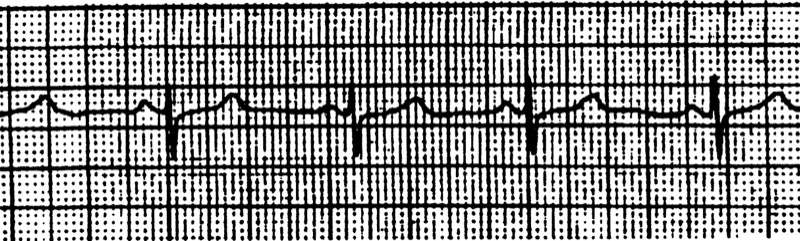
\includegraphics[width=0.618\textwidth]{pictures/ekg}
\end{center}
\caption{Graph eines EKG}\label{ekg}
\end{figure}

\begin{ueb}[EKG]
Jedes kleine Quadrat in der Figur entspricht $\unit[0.04]{s}$, jedes grosse Quadrat also $\unit[0.2]{s}$. Wie oft schlägt demnach das Herz der Versuchsperson in einer Minute?
\end{ueb}

Wir haben bereits die elementaren Funktionen $\sin, \cos$ und $\tan$ kennengelemt; sie sind periodisch mit der Periode $2\pi$ bzw. $\pi$.

\begin{ueb}[Modifizierte Wellen]
Zeichne in dasselbe Koordinatensystem die Graphen der Funktionen $x\mapsto$
\begin{enumeratea}
\item $\sin(2x), \sin(x/2)$,
\item $2\cos x, 0.5\cos x$,
\item $\sin(x + \pi/2), \sin(x - \pi/4)$,
\item $2\cos(x + \pi/3), 3\cos(x - \pi/2)$.
\end{enumeratea}
\end{ueb}

\begin{ueb}[Superposition]
Zeichne den Graphen der Funktion $f:x\mapsto$

\begin{minipage}{0.49\textwidth}
\begin{enumeratea}
\item $\sin x + \sin2x$,
\item $2\sin x - \cos2x$,
\end{enumeratea}
\end{minipage}
\begin{minipage}{0.49\textwidth}
\begin{enumeratea}
\addtocounter{enumi}{2}
\item $x+\sin x$,
\item $\tan x +1/\tan x$.\\
\end{enumeratea}
\end{minipage}

\noindent Hinweis: Zerlege den Funktionsterm in zwei Teile: $f(x)=f_1(x)+f_2(x)$ und zeichne zunächst die Graphen von $f_1$ und $f_2$ . Addiere dann die Ordinaten der Punkte mit derselben Abszisse (Superposition, Überlagerung) .
\end{ueb}

\begin{ueb}[Turn up the Heat]
Eine Fabrik, die 1000$x$ Heizkessel herstellt, rechnet damit, dass die Kosten
$$K( x )= 10000x( 200 + 20\sin(\frac{\pi}{12}x))$$
Franken betragen. Wie hoch sind die Kosten bei der Produktion von 18000 Kessel? Wie viele Kessel werden hergestellt, wenn die Kosten 4200000 betragen?
\end{ueb}

\begin{ueb}[brrrrr]
A mathematical model for the temperature in Fairbanks (Alaska) is
$$T(x) = 21\sin\left[\frac{2\pi}{365}(x - 101)\right] - 4 ,$$
where $T(x)$ is the temperature in degrees Celsius on day $x$, with $x=0$ corresponding to January 1 and $x=365$ corresponding to December 31. Calculate the temperature on January 1, March 1, May 22, July 5, December 31.
\end{ueb}

\begin{ueb}[Stausee]
Abbildung \ref{abb:stausee} auf Seite \pageref{abb:stausee} zeigt den Füllungsgrad der Schweizer Stauseen in Prozent (100\% entsprechen 8390 GWh) für den Winter 1990/91 und die Schwankungsbreite der hydrologischen Jahre 1971 bis 1989.

\begin{figure}
\begin{center}
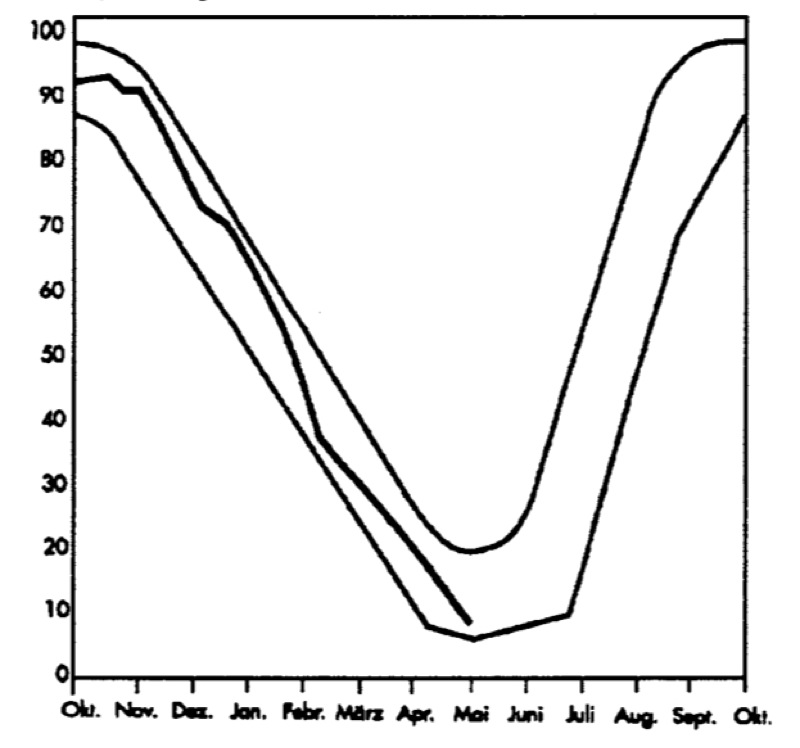
\includegraphics[width=0.7\textwidth]{pictures/stausee}
\end{center}
\caption{Füllgrad Schweizer Stauseen}\label{abb:stausee}
\end{figure}
Ermittle den Funktionsterm, der in Abhängigkeit der Zeit $t$ in Monaten den ungefähren Füllungsgrad in \% angibt.
\end{ueb}

\begin{ueb}[Biorhythmus]
Nach der Theorie der Biorhythmen sollen die Leistungen und das Verhalten eines Menschen in wellenförmigen Schwingungen verlaufen. Dabei unterscheidet man den physischen, den emotionalen und den intellektuellen Rhythmus. Der physische Rhythmus bezieht sich auf die körperliche Leistung und Ausdauer, seine Periode beträgt 23 Tage. Der emotionale Rhythmus wird mit der Seele, dem Wohlbefinden und der Lust und Laune in Verbindung gebracht. Seine Periode beträgt 28 Tage. Der intellektuelle Rhythmus bezieht sich auf den Verstand, das Erkenntnis- und Denkvermögen. Seine Periode beträgt 33 Tage. Alle Rhythmen können durch Sinus- oder Cosinuskurven beschrieben werden. Sie beginnen mit der Geburt. Heinz hat am 1. Januar 1993 bei allen Rhythmen den Höchststand erreicht.
\begin{enumeratea}
\item Gib einen Funktionsterm der Art
$$E(t) = a \cos(bt)$$
für den emotionalen Rhythmus so an, dass Werte von $-10$ bis $10$ angenommen werden (t in Tagen). Wie fühlt sich Heinz am 13. Mai?
\item Gib einen Funktionsterm der Art
$$I(t) = a + b \cos (ct)$$
für den intellektuellen Rhythmus so an, dass Werte von $0$ bis $100$ angenommen werden (t in Tagen). Welchen Wert erreicht Heinz am 22. Mai?
\end{enumeratea}
\end{ueb}

\begin{ueb}[ArcSin]
Die Sinusfunktion ist im Intervall $[-\frac{\pi}{2},\frac{\pi}{2}]$ monoton wachsend; sie hat also für dieses Intervall eine Umkehrfunktion. Ihr Name ist Arcus-Sinus und wird mit arcsin oder $\sin^{-1}$ bezeichnet.
$$f^{-1}(x)=\arcsin(x)$$
Überlege dir, welchen Wertebereich die Funktion hat und zeichne den Graphen von $\arcsin$ durch Spiegelung des Graphen von $\sin$ an der 1. Winkelhalbierenden.

\noindent Verfahre ebenso für $\cos$ und $\tan$.
\end{ueb}

\begin{figure}
\begin{center}

\includegraphics[width=0.618\textwidth]{pictures/telemetrie}
\end{center}
\caption{Duplo Telemetrie}
\end{figure}
 
\section{Potenzfunktionen}
  
\subsection{Potenzen mit rationalen Exponenten}
\subsubsection{Rückblick}
  \begin{wrapfigure}{r}{0.382\textwidth}
  \begin{center}
    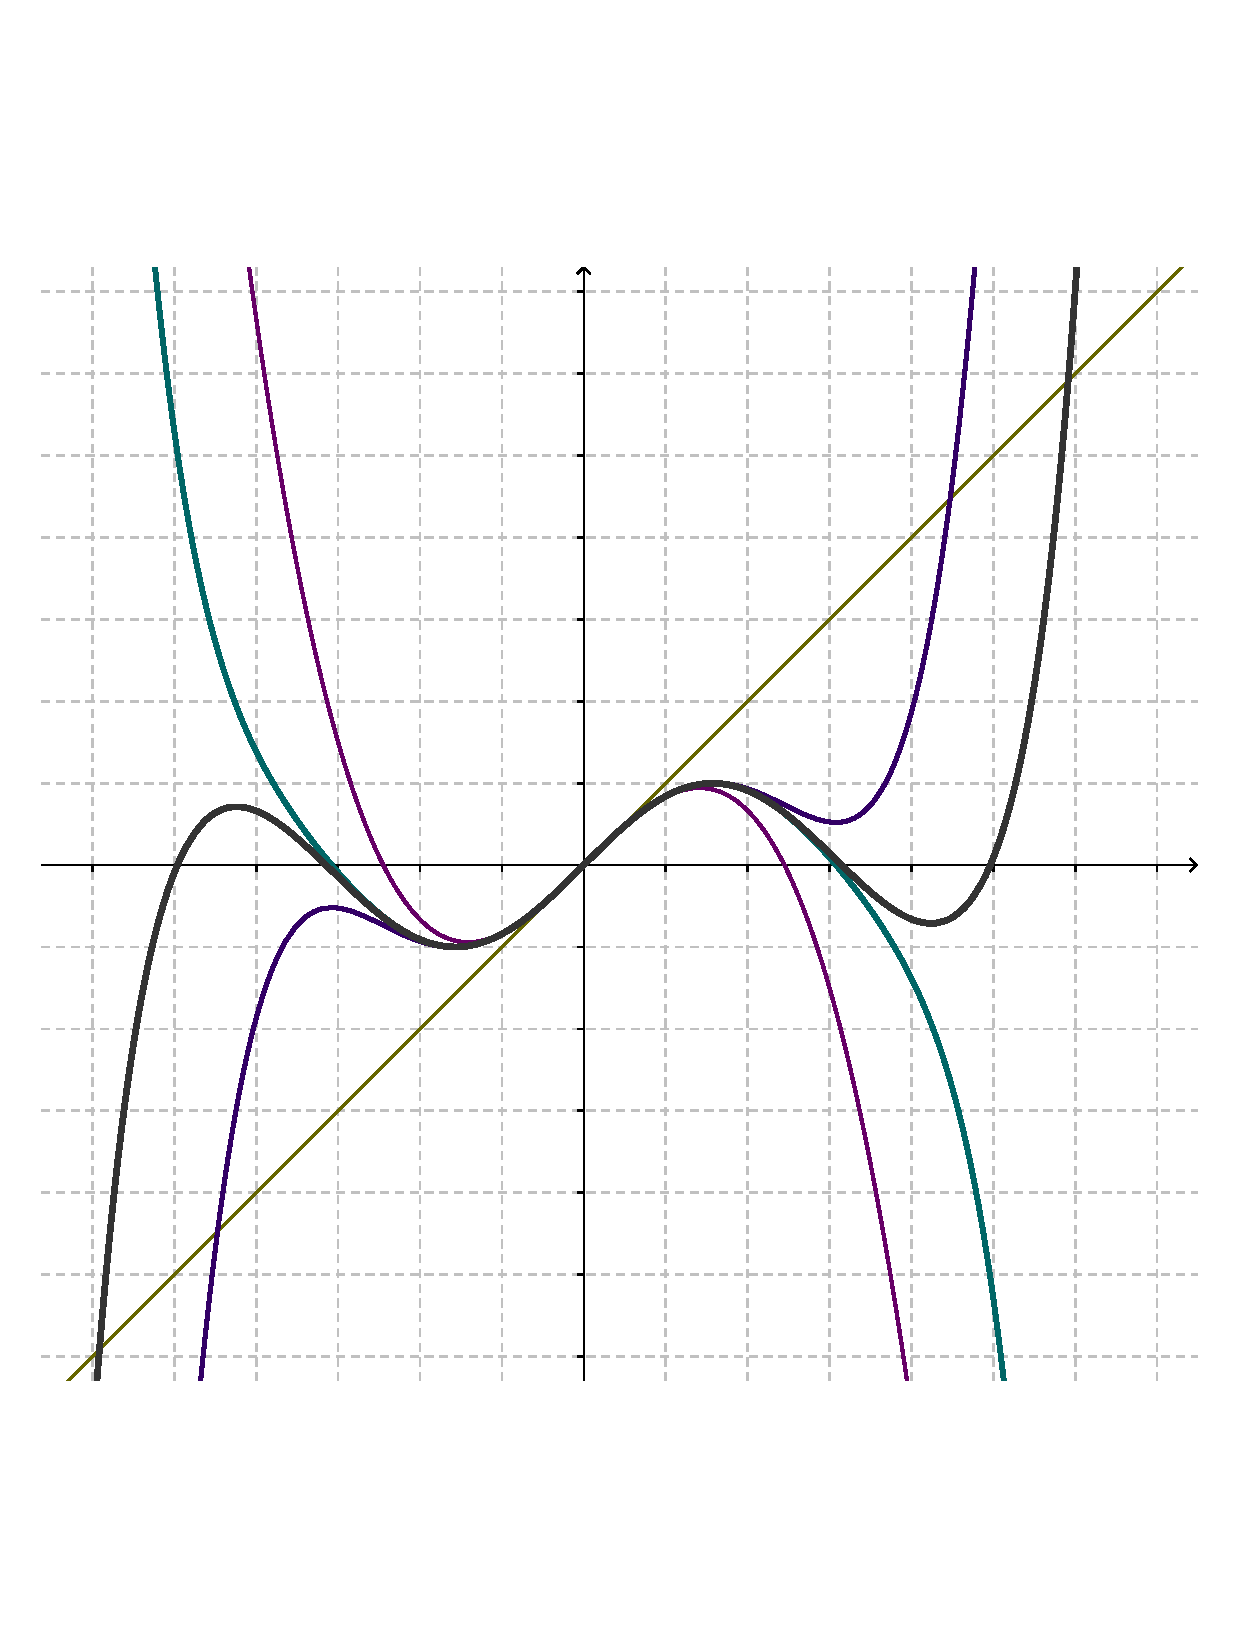
\includegraphics[width=0.382\textwidth]{pictures/title}
  \end{center}
\end{wrapfigure}
Wir wollen unsere Rechenregeln für Potenzen erweitern, um Potenzgesetze
für reelle Zahlen vollumfänglich verstehen und interpretieren zu können.
Wir brauchen dazu folgende, bereits bekannte, Regeln und Begriffe.
\begin{erin}
  Sie
\marginnote{
\qrcode{
https://www.youtube.com/watch?v=du2h6QDXNoo}
}
  kennen die Potenzgesetze. In Kurzform lauten sie:
\begin{align}
  a^n\cdot a^m&=a^{n+m}\\
  a^n\cdot b^n&=(ab)^n\\
  \left(a^n\right)^m&=a^{n\cdot m}\\
  a^{-n}&=\frac{1}{a^n}\\
  a^0&=1
\end{align}

Bisher waren die Exponenten $m$ und $n$ jeweils natürliche Zahlen. Im
nächsten Abschnitt werden wir sehen, dass auch rationale Zahlen Sinn
machen.

Weiter ruft man sich die Definition der $n$-ten Wurzel einer Zahl
in Erinnerung: Die \emph{$n$-te Wurzel} aus einer positiven Zahl
$a$, ist diejenige positive Zahl, deren $n$-te Potenz $a$ beträgt.
Man schreibt dafür $\sqrt[n]{a}$.
\end{erin}

\begin{mot}
  Die Potenzgesetze funktionieren bis anhin tadellos, wenn $m$ und
$n$ ganze Zahlen sind. Was ist, wenn man im Exponenten rationale
Zahlen zulässt? Ist $3^{\frac{1}{2}}$ eine Zahl? Wenn ja, welche?

Sollen die Potenzgesetze weiterhin gelten, dann ist
$3^{\frac{1}{2}}\cdot3^{\frac{1}{2}}=3^{\frac{1}{2}+\frac{1}{2}}=3^1=3$.
Also $3^{\frac{1}{2}}\cdot3^{\frac{1}{2}}=3$. Wir wissen, dass
$\sqrt{3}\cdot\sqrt{3}=3$ und legen deshalb fest:
$$3^{\frac{1}{2}}=\sqrt{3}.$$
\end{mot}

\begin{ueb}[Wurzeln]
  Bestimme nach obigem Muster die Wurzeldarstellung von
  $8^{\frac{1}{3}}$. Betrachte dazu $8^{\frac{1}{3}}$ dreimal
  mit sich selbst multipliziert.
\end{ueb}

\subsubsection{Erweiterung der Potenzgesetze}
Es zeigt sich, dass jede Wurzel als Potenz mit rationalem Exponenten
dargestellt werden kann. Man erweitert die Potenzgesetze deshalb
intuitiv auf rationale Exponenten und definiert:\pagebreak

\begin{cdef}[Wurzeln als Potenz]{}
  $$\boxed{\rule[-3mm]{0mm}{25pt}\quad a^{\frac{1}{n}}=\sqrt[n]{a}\quad}$$
\end{cdef}
\noindent Man kann also jede Wurzel in eine Potenz verwandeln und dann mit den
bekannten Potenzgesetzen rechnen. Dies ist beim Umformen und
Vereinfachen von Wurzeln enorm hilfreich.
Wir fassen unsere Überlegungen in einem Satz zusammen.
 
Weil wir mit Exponenten
wie mit rationalen Zahlen rechnen können gilt allgemein
\begin{csatz}[Potenzgesetz {\uppercase\expandafter{\romannumeral5}}]{}
  $$a^{\frac{n}{m}}=\sqrt[m]{a^n}$$
\end{csatz}

\begin{proof}[Beweis]
Schreibübung.
\end{proof}

\begin{ueb}[Potenzgesetze]
  Schreibe mit einer einzigen Wurzel.

(a) $\sqrt[3]{a\sqrt{a}}\q$ (b) $\sqrt[4]{a\sqrt[3]{a\sqrt{a}}}\q$ (c) $\sqrt[n]{\sqrt[m]{a}}\q$ (d) $\sqrt[n]{a}\cdot\sqrt[m]{a}$
\end{ueb}

\begin{ueb}[TR]
  Bestimme mit dem Taschenrechner folgende Werte

(a) $\sqrt[3]{10}\q$ (b) $\sqrt[6]{100}\q$ (c) $\sqrt[1000]{3}\q$ (d) $\sqrt[10^6]{3}$
\end{ueb}
\begin{ueb}[Gewicht]
  Berechnen Sie die Kraft, mit der ein Mensch der Masse $\unit[50]{kg}$ von
  der Erde angezogen wird.

(a) am Nordpol$\q$ (b) am Äquator
\end{ueb}
\begin{ueb}
  Rückblick. Berechnen Sie die Inversfunktion von $f(x)=\frac{1}{x}$.
\end{ueb}
\begin{ueb}[Wurzel $x$]
Führe mit dem TR für eine beliebige, positive Zahl folgendes Verfahren mehrmals durch:
\begin{itemize}
\item $x$ eintippen
\item $\sqrt{x}$ berechnen
\item das Resultat als neues $x$ nehmen
\end{itemize}
Gegen welchen Wert strebt $x$, wenn man diese Schleife oft ausführt?
\end{ueb}

\subsubsection{Potenzen mit irrationalen Exponenten}
Es ist möglich, Potenzen mit irrationalen Exponenten zu definieren.
Man tut dies mit einer Streckenschachtelung im Exponenten. Ohne
Beweis akzeptieren wir folgenden
\begin{csatz}[Irrationale Exponenten]
  Alle Potenzgesetze gelten auch für Potenzen mit irrationalen
  Exponenten.
\end{csatz}

Damit ist das Kapitel Potenzgesetze abgeschlossen; für das gymnasiale Momentum.

\begin{ueb}[ohne TR]
Bestimme ohne TR --- exakt oder näherungsweise --- folgende Werte.

(a) $\sqrt{10^6}\q$ (b) $\sqrt[\pi]{10^6}\q$ (c) $3^{\frac{\pi}{6.28}}\q$ (d) $64^{\frac{1}{\pi}}\q$ (e) $\pi^\pi\q$ (e) $\pi^{0.5}$
\end{ueb}

\subsection{Potenzfunktionen}
\begin{cdef}[Potenzfunktion]{}
Funktionen der Form
$$f(x)=x^n\q(n\in\mZ)$$
heissen \emph{Potenzfunktionen}.
\end{cdef}

\begin{ueb}[Graphen]
Zeichne in dasselbe Koordinatensystem die Graphen der Funktionen $x\mapsto$

(a) $x^2, x^4, x^{-2}, x^{-4}\q$ (b) $x^3, x^5, x^{-1}, x^{-3}.$
\end{ueb}

\begin{bem}
Die Graphen der Funktionen $f(x)=x^n$, für $n$ gerade,
sind achsensymmetrisch zur y-Achse, da für gerade Exponenten $(-x)^n=x^n$. Für $n$ ungerade, sind die Graphen punktsymmetrisch zum Ursprung des Koordinatensystems, da $(-x)^n=-x^n$.
\end{bem}

\begin{bem}
Potenzfunktionen mit negativen Exponenten $n$ sind für $x=0$ nicht definiert. Ihre Graphen bestehen aus zwei Ästen, die für gerade Exponenten symmetrisch zur $y$-Achse, für ungerade Exponenten symmetrisch zum Ursprung liegen. Für $x$-Werte von hinreichend grossem Betrag werden die Funktionswerte dem Betrage nach beliebig klein, d.h. der Graph kommt für solche $x$-Werte der $x$-Achse beliebig nahe. Man sagt: Die $x$-Achse ist \emph{Asymptote} des Graphen. Für hinreichend nahe bei $0$
gelegene $x$-Werte werden die Funktionswerte dem Betrage nach beliebig gross, d.h. der Graph kommt für solche $x$-Werte der $y$-Achse beliebig nahe. Die $y$-Achse ist ebenfalls eine Asymptote des Graphen. Die undefinierte Stelle $x=0$ nennen wir \emph{Polstelle}.
\end{bem}

\subsection{Wurzelfunktionen}
\begin{ueb}[Graphen 2]
Zeichne für $x\in\mR^+$ in dasselbe Koordinatensystem die Graphen der Funktionen

(a) $f(x)=x^2$ und $g(x)=x^\frac{1}{2}=\sqrt[2]{x}\q$ (b) $f(x)=x^3$ und $g(x)=x^\frac{1}{3}=\sqrt[3]{x}$
\end{ueb}
\begin{cdef}[Wurzelfunktion]{}
Funktionen der Form
$$f(x)=x^\frac{1}{n}=\sqrt[n]{x}\q(n\in\mZ\setminus\set{0})$$
heissen \emph{Wurzelfunktionen}.
\end{cdef}
Die Definitionsmenge der Wurzelfunktionen ist $\mR^+_0$. Sie sind für $\mR_0^+$ die Umkehrfunktionen von $f(x)=x^n$. Ihre Graphen entstehen deswegen aus den Graphen von $f$ durch Spiegelung an der 1. Winkelhalbierenden.

\begin{ueb}[Wurzeln]
Ermittle den Parameter $a$ so, dass der Graph von $f(x)=x^a$ durch den Punkt

(a) $P\point{2}{512}\q$ (b) $P\point{243}{3}\q$ (c) $P\point{-1}{-1}$
geht.
\end{ueb}

\begin{ueb}[Graphen 3]
Zeichne den Graphen der Quadratwurzelfunktion
$$f(x)=\sqrt{x}$$
für $0<x<10$ und die Parallele zur x-Achse durch den Punkt $P\point{0}{8}$. Schneidet die Kurve die Parallele, wenn man sie nach rechts fortgesetzt denkt? Wo?
\end{ueb}

\begin{ueb}[Wind]
Mit zunehmender Höhe nimmt die Windgeschwindigkeit zu. Für windschwache Gebiete kann man die gegenseitige Abhängigkeit durch die Funktion
$$f(x)=0.2\sqrt{x}+1$$
beschreiben. Dabei ist $x$ die Masszahl der in Meter gemessenen Höhe. Der Funktionsterm gibt die in $\nicefrac{m}{s}$ gemessene Windgeschwindigkeit an. Zeichne den Graphen der Funktion für $0<x<600$. In welcher Höhe erreicht die Windgeschwindigkeit $\unitfrac[7]{m}{s}$?
\end{ueb}

\begin{ueb}[Verschieben]
Zeichne den Graphen der Funktion
$$f(x)=\frac{1}{8}x^3.$$
Verschiebe den Graphen
\begin{enumeratea}
\item um 3 Einheiten nach oben,
\item um 2 Einheiten nach rechts,
\item um 2 Einheiten nach links und anschliessend um
1 Einheit nach unten.
\end{enumeratea}
Gib jeweils die Gleichung der neuen Kurve an.
\end{ueb}

\begin{ueb}[Schnittpunkte]
Zeichne die Graphen der Funktionen
$$f(x)=x^{-1}-2\q\text{und}\q g(x)=4-x^{-1}$$
in ein Koordinatensystem.
\begin{enumeratea}
\item Wo schneiden die Graphen die x-Achse?
\item Wo schneiden sich die beiden Graphen?
\end{enumeratea}
\end{ueb}

\begin{ueb}[Gebiete]
Zeichne für $x >0$ die Graphen der Funktionen
$$f(x)=2x^{0.5}\q g(x)=0.5x^{1.5}\q h(x)=2x^{-2}$$
in ein Koordinatensystem.
\begin{enumeratea}
\item Berechne die Schnittpunkte von je zwei dieser
drei Graphen.
\item In wie viel Gebiete wird die Ebene durch diese drei
Graphen geteilt?
\item Beschreibe dasjenige Gebiet durch Ungleichungen, in dem $P\point{2}{2}$ liegt.
\end{enumeratea}
\end{ueb}

\begin{ueb}[Konsum]
Die Konsumausgaben $C$ eines Haushalts hängen vom Haushaltseinkommen $Y$ in folgender Weise ab:
$$C(Y) =80\sqrt{0.2Y+36},$$
$Y$ und $C(Y)$ in $\unitfrac{Fr.}{Monat}$.
\begin{enumeratea}
\item Ermittle die mathematische Definitionsmenge der Konsumfunktion. Entspricht diese Menge der ökonomischen Definitionsmenge?
\item Wie hoch ist das Existenzminimum?
\item Von welchem Monatseinkommen an wird die monatliche Sparsumme positiv?
\item Bei welchem Monatseinkommen verbraucht der Haushalt für Konsumzwecke genau 90\% seines Einkommens? (Sparquote ist 10\%)
\end{enumeratea}
\end{ueb}

\begin{ueb}[Angebot \& Nachfrage]
Die Angebots- und Nachfragefunktion für ein wirtschaftliches Gut seien gegeben durch
$$p_A(x)=2x^\frac{1}{2},\q p_N(x)=4+\frac{2}{x},$$
$\unit[0]{ME}<\unit[x]{ME}<\unit[8]{ME}$, wobei die Preise in $\nicefrac{GE}{ME}$ angegeben sind. Stelle die Situation graphisch dar und lies die Gleichgewichtsmenge, den Marktpreis und den Gesamterlös ab.
\end{ueb}

\section{Exponentialfunktionen}

\subsection{Einleitung}
\begin{wrapfigure}{r}{0.3\textwidth}
  \begin{center}
    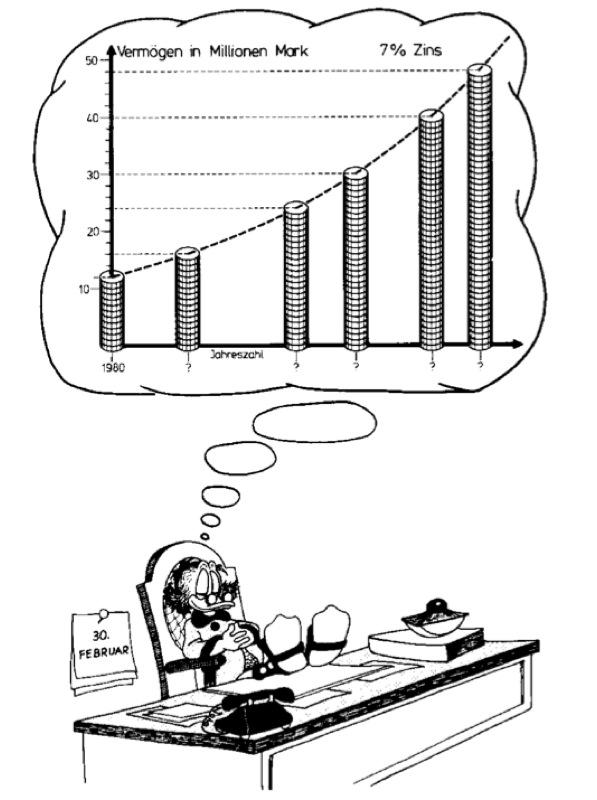
\includegraphics[width=0.2\textwidth]{pictures/dagobert}
  \end{center}
\end{wrapfigure}
Seit der Pandemie von SARS2 CoV19 im Jahr 2020 ist der Begriff des \emph{exponentiellen Wachstums} in aller Munde. Ein Beispiel aus einer Tageszeitung --- dem Tagesspiegel Ausgabe vom 12.3.21 --- fand ich hier:
    \href{https://www.tagesspiegel.de/wirtschaft/wie-exponentielles-wachstum-unser-leben-beeinflusst-4236517.html}{Wie exponentielles Wachstum unser Leben beeinflusst}
Dieser wichtige Typ Funktion soll nun in diesem Kapitel ergründet werden.

\begin{bsp}
Ein Schüler verbreitet zu Beginn der grossen Pause im Gymnasium Lerbermatt ein Gerücht. Alle Minuten erzählt ein Wissender einem Nicht-Eingeweihten das Gerücht. Wie lange dauert es, bis alle Schüler des Gymnasiums über das Gerücht in Kenntnis gesetzt worden sind?
\end{bsp}

Bei den Potenzfunktionen sind die Exponenten immer Konstanten, bei den Exponentialfunktionen ist die Basis konstant und der Exponent variabel.
\begin{cdef}[Exponentialfunktion]{}
Eine Funktion der Form
$$f(x)=b^x$$
mit $b\in\mR^+$ heisst \emph{Exponentialfunktion} zur Basis $b$.
\end{cdef}

\begin{bsp}
Anwendungen, die durch Exponentialfunktionen beschrieben werden sind:
\begin{itemize}
\item Ausbreitung von Krankheiten/Epidemien
\item Radioaktiver Zerfall
\item Zellvermehrung
\end{itemize}
\end{bsp}

\subsection{Graphen}
\begin{ueb}[Graphen]
\label{uebgraphen}
Zeichne in dasselbe Koordinatensystem die Graphen
der Funktionen\\

(a) $2^x$, $3^x$, $2.7^x\q$ (b) $4^x$, $\left(\frac{1}{4}\right)^x$, $10^x$
\end{ueb}

\begin{ueb}[Potenz vs Exponent]
Vergleiche das Verhalten (insbesondere das Wachstum) der beiden Funktionen
$$p(x)=x^2\q\text{und}\q e(x)=2^x$$
\end{ueb}

\begin{bem}
Der Graph der Exponentialfunktionen
$$f(x)=b^x$$
liegt oberhalb der x-Achse und geht durch den Punkt $\point{0}{1}$. Für $b>1$ ist der Graph steigend ($f$ monoton wachsend) und die negative $x$-Achse Asymptote; für $0<b<1$ ist der Graph fallend ($f$ monoton fallend) und die positive $x$-Achse Asymptote.
\end{bem}

\begin{csatz}[Wachstum- \& Zerfall]{}
Die Kurven mit den Gleichungen $y=b^x$ und $y=\left(\frac{1}{b}\right)^x$ liegen symmetrisch zueinander bezüglich der y-Achse.
\end{csatz}

\begin{proof}[Beweis]
Übung.
\end{proof}

\begin{ueb}[durchschnittliche Änderung]
Berechne für die Funktionen der Übung \ref{uebgraphen} die durchschnittlichen Steigungen in den Intervallen $[0,1]$ und $[-1,0]$.
\end{ueb}

\begin{ueb}[Verschieben]
Zeichne den Graphen von $f(x)=2^x$ in ein Koordinatensystem.
\begin{enumeratea}
\item Verschiebe den Graphen in positiver x-Richtung
um 3 Einheiten.
\item Spiegele den Graphen an der x-Achse.
\item Verschiebe den Graphen in negativer y-Richtung
um 4 Einheiten.
\item Spiegele den Graphen an der y-Achse.
\item Spiegele den Graphen am Ursprung des Koordinatensystems.
\end{enumeratea}
Geben Sie jeweils die Gleichung der Bildkurve an.
\end{ueb}

\begin{figure}
  \begin{center}
    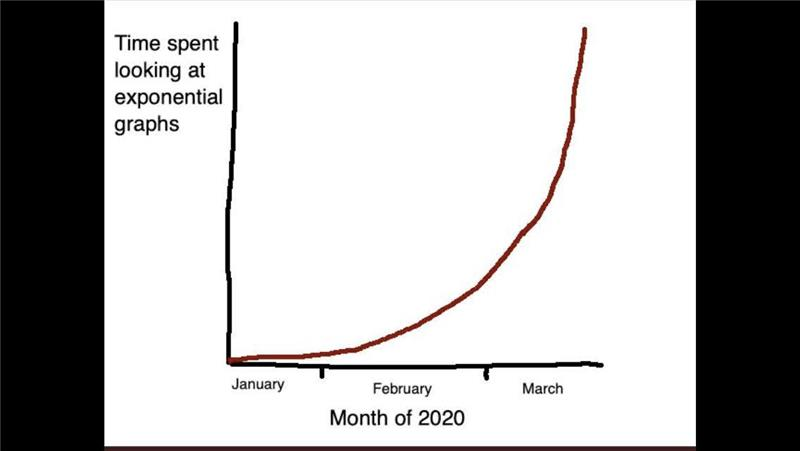
\includegraphics[width=0.618\textwidth]{pictures/exponentialgraphs.jpg}
    \caption{Joke During SARS2-CoV19 Lockdown in 2020}
  \end{center}
\end{figure}

\begin{ueb}[Exponent]
Es sei
$$f(x)=b^x\text{ und }g(x)=a\cdot b^x.$$
Der Punkt $P$ liegt auf dem Graphen von $f$. Berechne $b$ für
\begin{enumeratea}
\item $P=\point{1.5}{27}$
\item $P=\point{4}{9}$
\end{enumeratea}
Die Punkte $R$ und $Q$ liegen auf dem Graphen von $g$. Berechne $a$ und $b$ für
\begin{enumeratea}
\setcounter{enumi}{2}
\item $R\point{0}{2}, Q\point{2}{18}$
\item $R\point{-2}{20}, Q=\point{3}{\frac{5}{8}}$
\end{enumeratea}
\end{ueb}

\subsection{Wachstum und Zerfall}
Die Exponentialfunktionen spielen bei der Beschreibung von zeitabhängigen Wachstums- und Zerfallserscheinungen eine ausserordentlich wichtige Rolle.
\begin{cdef}[Exponentialfunktion allgemein]{}
  Ist $t$ die Masszahl der Zeit, so bezeichnet man die Funktion
$$f(t)=ab^t$$
für $b>1$ als \emph{exponentielle} Wachstumsfunktion, für $0<b<1$
als exponentielle Zerfallsfunktion.
\end{cdef}
\begin{bem}
Zum Zeitpunkt $t=0$ gilt
$$f(0)=ab^0=a.$$
Also ist $(0|a)$ der Schnittpunkt mit der $y$-Achse, und man nennt $a$ den Anfangswert von $f$. Der Parameter $b$ ist ein Mass für das Wachstum bzw. den Zerfall und wird deshalb Wachstums- bzw. Zerfallsfaktor genannt.
\end{bem}

\begin{ueb}[Bakterien]
Bei einer Bakterienkultur ohne Raum- und Nahrungsmangel wächst die Individuenzahl exponentiell. Um 8 Uhr waren es 2300 und um 12 Uhr 36800 Individuen.
\begin{enumeratea}
\item Nimm 2300 als Anfangswert an und ermittle den Wachstumsfaktor $b$. Wie lautet demnach die entsprechende Wachstumsfunktion?
\item Welches ist die Individuenzahl um 9 Uhr, um 11 Uhr, um 13.30 Uhr?\label{bakterienb}
\end{enumeratea}
\end{ueb}

\begin{ueb}[Wald]
Ein Waldbestand, in dem kein Holz geschlagen wird, wächst exponentiell. Er beträgt heute $\unit[72\,342]{m^3}$, vor zwölf Jahren betrug er $\unit[48\,228]{m^3}$.
\begin{enumeratea}
\item Wie hoch war der Waldbestand vor fünf Jahren?
\item Wie hoch wird er heute in sieben Jahren sein?
\end{enumeratea}
\end{ueb}

\begin{ueb}[Bakterienkultur]
In einer Bakterienkultur ist $$f(t) =10^4 \cdot 2^\frac{t}{2}$$ die Anzahl der Bakterien zum Zeitpunkt $t$. In welcher Zeitspanne $\Delta t$ verdoppelt, vervierfacht, verachtfacht sich die Anzahl?
\end{ueb}

\begin{bem}
In der Praxis werden viele Wachstumsprozesse dadurch beschrieben, dass man neben dem Startwert $a$ noch die jährliche Zunahme der betrachteten Grösse in Prozenten angibt. Man denke einfach an die wohlbekannte Zinseszinsrechnung.
\end{bem}

\begin{bsp}
Es sei $f(0)=a=10000$ die Anzahl der Einwohner einer Stadt, deren jährliches Wachstum $2\%$ beträgt. Nach einem Jahr hat die Stadt $$f(1)=f(0)+0.02\cdot f(0)=f(0)\cdot(1+0.02)=10200$$ Einwohner. Nach zwei Jahren sind es
$$f(2)=f(1)\cdot(1+0.02)=f(0)\cdot(1+0.02)^2$$ Einwohner und analog nach $t$ Jahren
$$f(t)=10000\cdot1.02^t$$ Einwohner.
\end{bsp}

\begin{ueb}[Schweiz]
Vom Jahr 1875 zum Jahr 1985 ist die Wohnbevölkerung der Schweiz von 2\,750\,300 auf 6\,455\,900 angewachsen. Wieviel Prozent betrug die jährliche Zunahme, wenn man annimmt, dass die Bevölkerung von Jahr zu Jahr gleich viele Prozent zugenommen hat?
In Wirklichkeit verlief die Zunahme unregelmässig; siehe dazu Tabelle \ref{tab:bevoelkerung} auf Seite \pageref{tab:bevoelkerung}.
\definecolor{Gray}{gray}{0.9}
%\definecolor{darkgreen}{rgb}{0,0.4,0}
\definecolor{lightyellow}{rgb}{1,1,0.8}
%\arrayrulecolor{darkgreen}
%\doublerulesepcolor{black}
\begin{table}
\small
\begin{center}
\begin{tabular}{|c|c|}
\hline
\rowcolor{Gray}\spaltenheight Jahr & Zunahme in Prozent\spaltensep\hline
\rowcolor{lightyellow}\spaltenheight 1875 & 0.78\spaltensep\hline
\rowcolor{Gray}\spaltenheight 1902 & 1.15\spaltensep\hline
\rowcolor{lightyellow}\spaltenheight 1918 & -0.06\spaltensep\hline
\rowcolor{Gray}\spaltenheight 1937 & 0.36\spaltensep\hline
\rowcolor{lightyellow}\spaltenheight 1948 & 0.84\spaltensep\hline
\rowcolor{Gray}\spaltenheight 1965 & 1.01\spaltensep\hline
\rowcolor{lightyellow}\spaltenheight 1976 & 0.27\spaltensep\hline
\end{tabular}
\end{center}
\normalsize
\caption{Zunahme der Wohnbevölkerung der Schweiz}\label{tab:bevoelkerung}
\end{table}
\end{ueb}

\begin{ueb}[Kapital]
Leiten
\marginnote{
\qrcode{
https://www.youtube.com/watch?v=tMT4Nvru6xY}
}
Leite die Formel für das Kapital $K(n)$ nach $n$ Jahren in Abhängigkeit des Startkapitals $K_0$ und Zinsfusses $p$ her. Vergleichen Sie mit der Formelsammlung.
\end{ueb}

\begin{ueb}[Susanna]
Susanne erhält zur Eröffnung eines Jugendsparbuches von ihrer Bank zu ihrer Einlage von 100 Franken ein Eröffnungsgeschenk von 50 Franken. Über welchen Betrag wird sie bei einem Jahreszins von $5.5\%$ in 10 Jahren verfügen können?
\end{ueb}

\begin{ueb}[Manhatten]
Im Jahre 1627 wurde die Insel Manhattan (New York) für 24\$ den Indianern abgekauft. Im Jahre 1970 betrug der Wert nur des Landes 6 Milliarden Dollar. Welches ist die konstant angenommene jährliche Wertzunahme in Prozent?
\end{ueb}

\begin{ueb}[Toto]
Ein 57 jähriger Fussballfan und seine 59 jährige Schwester teilen einen Totogewinn von 50000 Franken so, dass sie im Zeitpunkt der Pensionierung (Frauen: 62 Jahre, Männer: 65 Jahre) gleich viel besitzen. Wieviel erhält jedes der Geschwister bei einem Zinssatz von 4.5\%?
\end{ueb}

\section{Logarithmen}
\begin{bsp}
Nach welcher Zeit $t$ sinkt die Menge $m_0$ eines radioaktiven Stoffes mit der Halbwertszeit $T=\unit[30]{y}$ auf einen Zehntel des ursprünglichen Wertes? Wir bezeichnen die Zeit mit $t$ und nehmen als Einheit $\unit[30]{y}$, die Masse zu Beginn sei $m_0$. Also haben wir für die Restmasse $m$ zur Zeit $t$:
$$m(t)=m_0\cdot\left(\frac{1}{2}\right)^t.$$
Um zu berechnen, wann noch $\frac{m_0}{10}$ übrig sind, lösen wir die zugehörige Gleichung nach $t$ auf:
    \begin{align*}
    \frac{m_0}{10}&=m_0\cdot\left(\frac{1}{2}\right)^t\tag{$\div m_0$}\\
    \frac{1}{10}&=\left(\frac{1}{2}\right)^t\tag{$()^{-1}$}\\
    10&=2^t
    \end{align*}
    Das Auflösen nach $t$ gelingt uns leider nicht, weil die gesuchte Variable
    im Exponenten steht; Wir sind gezwungen zu raten. Wegen
    $2^3<10<2^4$ ist $3<t<4$, und man findet rasch als Näherung
    $$t\approx3.32$$    
\begin{figure}
\begin{center}
\definecolor{cqcqcq}{rgb}{0.75,0.75,0.75}
\begin{tikzpicture}[line cap=round,line join=round,>=triangle 45,x=1.2cm,y=4.2cm]
\draw [color=cqcqcq,dash pattern=on 2pt off 2pt, xstep=0.6cm,ystep=1.05cm] (-0.1,-0.01) grid (5.9,1.01);
\draw[->,color=black] (-1,0) -- (6,0);
\foreach \x in {1,2,3,4,5}
\draw[shift={(\x,0)},color=black] (0pt,2pt) -- (0pt,-2pt) node[below] {\footnotesize $\x$};
\draw[color=black] (5.85,0.01) node [anchor=south west] {$\nicefrac{30t}{\text{y}}$};
\draw[->,color=black] (0,-0.2) -- (0,1.2);
\foreach \y in {0.25,0.5,0.75,1}
\draw[shift={(0,\y)},color=black] (2pt,0pt) -- (-2pt,0pt) node[left] {\footnotesize $\y$};
\draw[color=black] (0.05,1.15) node [anchor=west] {$\nicefrac{f(t)}{m_0}$};
\clip(-1,-0.2) rectangle (6,1.2);
\draw[line width=1.2pt, smooth,samples=50,domain=0.0:6.0] plot(\x,{1/(2^(\x))});
\end{tikzpicture}
\end{center}
\caption{Radioaktiver Zerfall}\label{zerfall}
\end{figure}
   Antwort: Man hat nach ca. $\unit[99.6]{y}$
    noch einen Zehntel der ursprünglichen Masse.
    \end{bsp}
  Diese Lösung ist unbefriedigend, da wir $t$ nicht genau bestimmen
  konnten. Das Problem liegt darin, dass wir zur Exponentialfunktion $f(x)=2^x$ zwar den $y$-Wert $10$ kennen, nicht aber den $x$-Wert. Wir suchen also die Inversfunktion der Exponentialfunktion $2^x$, die zu gegebenem $y$-Wert den ursprünglichen $x$-Wert liefert. Wie das geht kommt im nächsten Abschnitt.
  
\subsection{Die Logarithmusfunktion}
  \begin{wrapfigure}{r}{0.5\textwidth}
  \begin{center}
    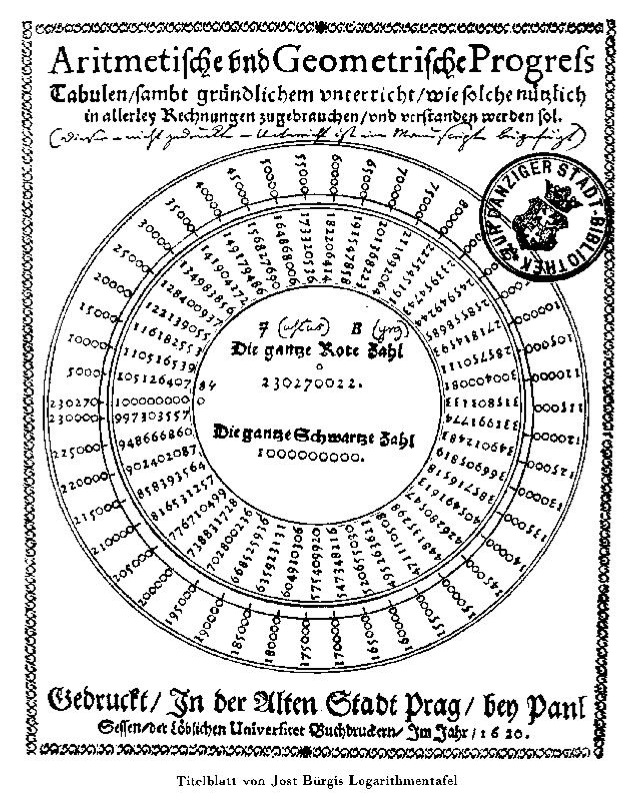
\includegraphics[width=0.37\textwidth]{pictures/logarithmentafel}
  \end{center}
\end{wrapfigure}
Wir möchten also eine gegebene Gleichung mit Variable im Exponenten lösen können. Dafür gehen wir von den bereits bekannten Exponentialfunktionen aus. Die Exponentialfunktion
$$f(x)=b^x$$
ist für $0<b<1$ streng monoton fallend und für $b>1$ streng monoton wachsend. Deshalb existiert eine Umkehrfunktion $f^{-1}$. Diese nennt man Logarithmusfunktion zur Basis $b$ und bezeichnet sie mit $\log_b$.

\begin{ueb}[Existenz der Inversfunktion]
Wie lautet das Kriterium für die Existenz einer Inversfunktion? Nenne eine Funktion, welche keine Inversfunktion besitzt.
\end{ueb} 

\begin{ueb}[check Spiegelung]
Zeichne die Funktion $f(x)=2^x$ und den Graphen der Inversfunktion $f^{-1}(x)=\log_2(x)$. Siehst du den bekannten graphischen Zusammenhang zwischen Funktion und Inversfunktion?
\end{ueb}

\begin{ueb}[verschieben]
Betrachte den Graphen der Funktion $f(x)=\log_2(x)$ in einem Koordinatensystem.
\begin{enumeratea}
\item Verschiebe den Graphen in positiver x-Richtung um 2 Einheiten.
\item Spiegle  den Graphen an der x-Achse.
\end{enumeratea}
Gib jeweils die Gleichung der Bildkurve an.
\end{ueb}

\begin{wrapfigure}{r}{0.3\textwidth}
\begin{center}
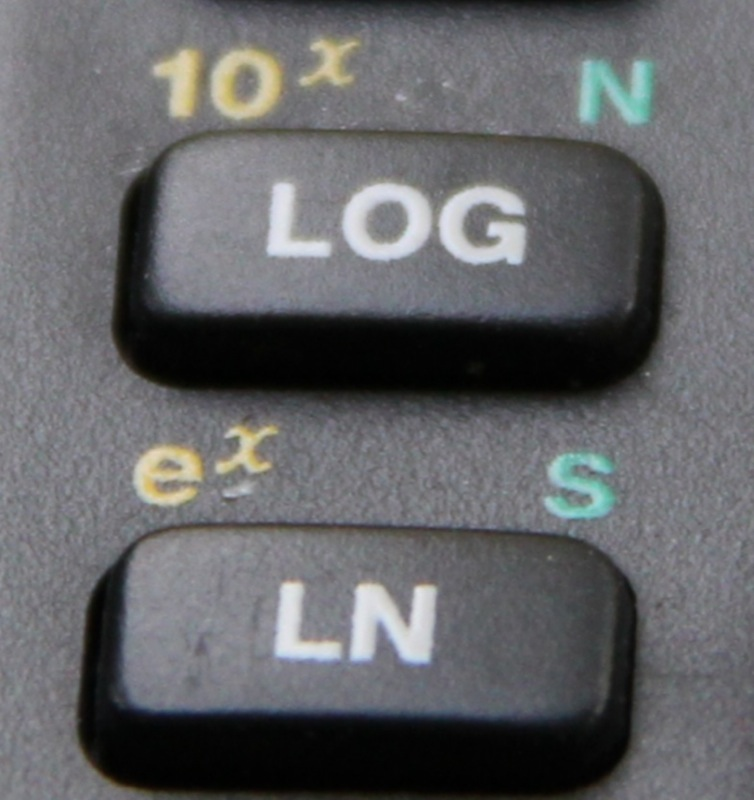
\includegraphics[width=0.2\textwidth]{pictures/logln}
\end{center}
\end{wrapfigure}
Mit der \fbox{log}-Taste kann man Werte von Variablen in
Exponenten bestimmen. Um sie korrekt
einsetzen zu können, wollen wir erst definieren, was wir unter einem Logarithmus verstehen wollen. Die Definition entspricht grundsätzlich einer Regel zum Umschreiben von Exponentialfunktionen.
\begin{cdef}[Logarithmus]{}
  Unter
\marginnote{
\qrcode{
https://www.youtube.com/watch?v=3LtdUV1l33g}
}
  dem \emph{Logarithmus} von $y$ zur Basis $b$, geschrieben
  $$\log_b{y},$$ versteht man diejenige Zahl, welche als Exponent
  der Basis $b$ den Wert $y$ ergibt. Mathematisch notiert wird diese
  Aussage übersichtlich:
  $$x=\log_b{y}\quad \Leftrightarrow \quad b^x=y.$$
  $y$ nennt man \emph{Numerus} und $b$ \emph{Basis} des Logarithmus.
\end{cdef}

\begin{bem}
  Bei Betrachtung obiger Äquivalenz wird klar, dass der Logarithmus nur für $y,b\in\D{R}^+$ und $b\neq1$
  definiert ist.
\end{bem}

\begin{ueb}[check Definitionsbereich]
Überlege kurz, welche Probleme entstünden, wenn man $y,b\in\mR$ zulassen würde.
\end{ueb}

\begin{bsps}
\ \\[-3ex]
  \begin{itemize}
    \item Den Logarithmus von $y$ zur Basis $b$ finden, ist gleichwertig
    mit der Beantwortung der Frage: \glqq $b$ hoch was gibt $y$?\grqq
    \item $\log_2{8}=3$: Der Logarithmus von $8$ zur Basis $2$ ist $3$,
    denn $2^3=8$.
    \item $\log_{10}{100}=2$, weil $10^2=100$.
    \item $\log_{\frac{1}{3}}{\frac{1}{9}}=2$, da
    $(\frac{1}{3})^2=\frac{1}{9}$.
  \end{itemize}
\end{bsps}

\begin{ueb}[Kopfrechnen]
Bestimme

\begin{minipage}{0.49\textwidth}
\begin{enumeratea}
\item $\log_{10}1000$, $\log_{10}1000000$, $\log_{10}10^6$, $\log_{10}10^{837}$
\item $\log_{10}0.1$, $\log_{10}0.01$, $\log_{10}\frac{1}{10}$, $\log_{10}\frac{1}{100}$
\end{enumeratea}
\end{minipage}
\begin{minipage}{0.49\textwidth}
\begin{enumeratea}
\setcounter{enumi}{2}
\item $\log_{2}4$, $\log_{2}1024$, $\log_{2}\frac{1}{4}$, $\log_{2}\frac{1}{512}$
\item $\log_{e}1$, $\log_{e}e$, $\log_{e}e^3$, $\log_{e}\frac{1}{e^4}$
\end{enumeratea}
\end{minipage}
\end{ueb}
Der folgende Satz folgt direkt aus der Definition und
bringt meine saloppe Formulierung aus dem obigen Beispiel auf den
Punkt.
\begin{csatz}[Exponenten-Eigenschaft]{}
  Jeder Logarithmus ist ein Exponent.
\end{csatz}

\begin{proof}[Beweis]
trivial
\end{proof}

\subsection{Übliche Bezeichnungen und Schreibweisen}

Erstens werde ich anstelle von $\log_b(y)$ nun oft $\log_b(x)$ schreiben. Das $y$ habe ich verwendet, um klar darzustellen, dass der Logarithmus $x=\log_b(y)$ die Umkehrfunktion einer Exponential\-funktion $y=b^x$ ist. In andern Worten wird hier der Schritt \glqq Vertauschung der Variablen\grqq --- der ja beim Algorithmus zur Bestimmung von Inversfunktionen als letzter erfolgt ---  schliesslich vorgenommen.
Zweitens kommt als Basis $b$ des Logarithmus
$$\log_bx$$
oft eine der drei Zahlen $2$, $e$ (Euler'sche Zahl) oder $10$ vor. Deshalb legt man folgende,
kürzere Schreibweisen fest:
\begin{itemize}
  \item $\log_{10}x=\log{x}=\lg x$\hfill(10$^{\text{er}}$ Logarithmus)
  \item $\log_\mathrm{e}{x}=\ln{x}$\hfill(Logarithmus naturalis)
  \item $\log_2{x}=\lb{x}$\hfill(Logarithmus dualis)
\end{itemize}
\begin{bem}
  Die \fbox{log} - Taste auf dem Taschenrechner ist also der
  Logarithmus zur Basis $10$.
\end{bem}
Drittens werde ich oft die Klammer um den Numerus weglassen, falls das Argument der Logarithmusfunktion klar ersichtlich ist. So wie das unter \glqq Zweitens\grqq\ bereits geschehen ist. Manchmal schreibe ich den Numerus in Klammer, um deutlich zu
kennzeichnen, was alles zum Logarithmus gehört. Zum Beispiel
$$\log_{3.5}(4x^3+2x-1).$$

\begin{ueb}[Graphen]
Lasse von \href{geogebra.org}{Geogebra} folgende Logarithmusfunktionen zeichnen.
\begin{itemize}
\item $f(x) = \log (x)$
\item $g(x) = \ln (x)$
\end{itemize}
\end{ueb}

\begin{figure}
\begin{center}
\definecolor{qqzzww}{rgb}{0,0.2,1}
\definecolor{zzqqtt}{rgb}{0.6,0,0.4}
\definecolor{cqcqcq}{rgb}{0.75,0.75,0.75}
\begin{tikzpicture}[line cap=round,line join=round,>=triangle 45,x=0.8cm,y=0.8cm]
\draw [color=cqcqcq,dash pattern=on 3pt off 3pt, xstep=1.6cm,ystep=1.6cm] (-1.4,-4.86) grid (11.72,4.7);
\draw[->,color=black] (-1.4,0) -- (11.72,0);
\foreach \x in {1,2,3,4,5,6,7,8,9,10,11}
\draw[shift={(\x,0)},color=black] (0pt,2pt) -- (0pt,-2pt) node[below] {\footnotesize $\x$};
\draw[color=black] (11.38,0.08) node [anchor=south west] { $x$};
\draw[->,color=black] (0,-4.86) -- (0,4.7);
\foreach \y in {-4,-3,-2,-1,1,2,3,4}
\draw[shift={(0,\y)},color=black] (2pt,0pt) -- (-2pt,0pt) node[left] {\footnotesize $\y$};
\draw[color=black] (0.1,4.3) node [anchor=west] { $y$};
\clip(-1.4,-4.86) rectangle (11.72,4.7);
\draw[smooth,samples=100,domain=0.01:11.72, line width=0.5mm] plot(\x,{ln(\x)});
\draw[color=zzqqtt, smooth,samples=100,domain=0.01:11.72, line width=0.35mm] plot(\x,{ln(\x)/ln(2)});
\draw[color=qqzzww, smooth,samples=100,domain=0.01:11.72, line width=0.35mm] plot(\x,{ln(\x)/ln(10)});
\draw[color=black] (9.5,1.8) node {$\ln$};
\draw[color=zzqqtt] (9.5,2.8) node {$\lb$};
\draw[color=qqzzww] (9.5,0.5) node {$\log$};
\end{tikzpicture}
\end{center}
\caption{Die Graphen von $\ln(x)$, $\log(x)$, und $\lb(x)$}
\end{figure}

\begin{ueb}[Wachstum]
Die Funktion
$$f(x)=\log_b(x)$$
ist für $b >1$ eine monoton wachsende Funktion. Allerdings ist dieses Wachstum sehr langsam. Um einen Eindruck davon zu bekommen, denke man sich ein Koordinatensystem, dessen $x$-Achse mehrere Äquatorumfänge lang ist.
Die Einheit sei $\unit[1]{cm}$. Überprüfe die Abbildung \ref{logvsaequator} für den Graphen von $\log(x)$ und zeichne die Werte von zwei weiteren \glqq Erdumrundungen\grqq\ in Abbildung \ref{logvsaequator} auf Seite \pageref{logvsaequator} ein.

\begin{figure}
\begin{center}
\definecolor{cqcqcq}{rgb}{0.75,0.75,0.75}
\begin{tikzpicture}[line cap=round,line join=round,>=triangle 45,x=0.6cm,y=0.6cm]
\draw [color=cqcqcq,dash pattern=on 2pt off 2pt, xstep=1.2cm,ystep=1.2cm] (-0.84,-0.62) grid (12.86,11.66);
\draw[->,color=black] (-0.84,0) -- (12.86,0);
\foreach \x in {,1,2,3,4,5,6,7,8,9,10,11,12}
\draw[shift={(\x,0)},color=black] (0pt,2pt) -- (0pt,-2pt) node[below] {\footnotesize $\x$};
\draw[color=black] (12.52,0.08) node [anchor=south west] { x};
\draw[->,color=black] (0,-0.62) -- (0,11.66);
\foreach \y in {,1,2,3,4,5,6,7,8,9,10,11}
\draw[shift={(0,\y)},color=black] (2pt,0pt) -- (-2pt,0pt) node[left] {\footnotesize $\y$};
\draw[color=black] (0.1,11.26) node [anchor=west] { y};
\clip(-0.84,-0.62) rectangle (12.86,11.66);
\draw[smooth,samples=100,domain=0.0:12.86] plot(\x,{9.6});
\draw[smooth,samples=100,domain=0.2:12.86] plot(\x,{ln(\x)/ln(10)});
\draw[color=black] (6,9) node {nach der 1. Erdumrundung};
\end{tikzpicture}
\end{center}
\caption{Log der Äquator-Vielfachen}\label{logvsaequator}
\end{figure}
\end{ueb}

\begin{ueb}[tippen ist leicht]
  Berechne mit dem TR folgende Logarithmen, und kontrolliere deine Berechnung, indem du $10$ \glqq hoch\grqq\ dein jeweiliges Resultat eintippst.\\
  
  \begin{minipage}{0.49\textwidth}
    \begin{enumeratea}
      \item $\log{7}$
      \item $\log{1001}$
      \item $\log{1024}$
    \end{enumeratea}
  \end{minipage}
  \begin{minipage}{0.49\textwidth}
    \begin{enumeratea}\addtocounter{enumi}{3}
      \item $\log{0.101}$
      \item $\log{10^{-23}}$
      \item $\log{0.5}$
    \end{enumeratea}
  \end{minipage}
\end{ueb}

\subsection{Rechenregeln}
Wir werden in Kürze Graphen von Logarithmen zu beliebigen Basen anschauen.
Damit wir aber mit dem TR Logarithmenfunktionen zu beliebigen Basen $b$
erstellen können (wir haben ja bloss die $\log$- und die $\ln$-Taste),
brauchen wir Umformungsregeln.

\subsection{Die Logarithmensätze}
Es folgen vier Logarithmenregeln. Die erste ist hilfreich beim
Eintippen in den Taschenrechner. Die letzte beschreibt, wie man
Gleichungen nach einer im Exponenten stehenden Variablen auflöst. Damit werden Sie dann in der Lage sein, für unser Ausgangsproblem auf Seite 1 den exakten Wert von $t$ zu bestimmen.

Die erste Regel besagt, dass jeder Logarithmus zu einer beliebigen Basis $b$ als Quotient von
Logarithmen zu einer beliebigen Basis $n$ geschrieben werden kann.
\begin{csatz}[Basiswechsel]{\label{satz:logtr}}\label{satz:logtr}
\marginnote{
\qrcode{
https://www.youtube.com/watch?v=79ax8cwhggk}
}
  $$\log_b{x} = \frac{\log_n{x}}{\log_n{b}}$$
\end{csatz}
Um diesen Satz zu beweisen, brauchen wir eine der folgenden drei Rechenregeln,
die leicht mit der Definition nachgewiesen werden können.\pagebreak

\begin{csatz}[Rechenregeln für Logarithmen]{}
Es
\marginnote{
\qrcode{
https://www.youtube.com/watch?v=xzwY11unPRI}
}
gilt
\begin{align}
  \log_b{(u\cdot v)}&=\log_b{u} + \log_b{v}\\[1ex]
  \log_b{\dfrac{u}{v}}&=\log_b{u} - \log_b{v}\\[1ex]
  \log_b{u^n}&=n\cdot\log_b{u}
\end{align}
\end{csatz}

\begin{proof}[Beweis]
  Nach Definition; also Übung. Hinweis: Erinnere dich daran, dass ein Logarithmus die Inversfunktion einer Exponentialfunktion ist und daher die Gesetze ähnlich zu den Potenzgesetzen sein müssen.
\end{proof}
\begin{proof}[Beweis zu Satz \ref{satz:logtr}]
  Es sei $\log_b{x} = y$, also
  $b^y=x$. Diese Exponentialgleichung logarithmieren wir auf beiden Seiten
  $$\log_n{b^y}=\log_n{x}.$$ Mit der dritten Logarithmenregel folgt dann
  $y\cdot\log_n{b}=\log_n{x}\q \Leftrightarrow\q
  y=\frac{\log_n{x}}{\log_n{b}}$
  Daraus folgt unmittelbar die Behauptung.
\end{proof}

\subsection{Graphen von Logarithmenfunktionen}
Sie haben ein
paar Graphen anhand von Wertetabellen oder mit \href{www.geogebra.org}{Geogebra}

\begin{ueb}[$e$]
  Skizziere die Graphen der Funktionen $f(x)=\log_e(x)$ und
  $g(x)=\log_{\frac{1}{e}}(x)$ in ein und dasselbe
  Koordinatensystem. Was fällt auf?
\end{ueb}

\begin{ueb}[Und immer wieder grüsst die Inversfunktion.]
Skizziere die Graphen der Funktionen $f(x)=\ln x$ und $g(x)=e^x$ in ein und dasselbe Koordinatensystem. Was fällt auf? Erkläre das Ergebnis.
\end{ueb}

\begin{ueb}[Kopfrechnen 2]
Vereinfache
$e^{\ln 2}$, $\ln(e^2)$, $e^{\ln(x)}$, $\ln(e^x)$?
\end{ueb}

\begin{csatz}[Eigenschaften der Logarithmusfunktion]{}
  Graphen von Logarithmusfunktionen haben folgende Eigenschaften:
  \begin{itemize}
    \item Sie gehen alle durch den Punkt $\point{1}{0}$.
    \item Die Graphen von $f(x)=\log_b{(x)}$ und
    $g(x)=\log_{\frac{1}{b}}{(x)}$ sind achsialsymmetrisch bezüglich
    der x-Achse.
  \end{itemize}
\end{csatz}

\begin{proof}[Beweis]
  Wir betrachten eine beliebige Logarithmusfunktion $f(x)=\log_b(x)$.
  Also $f(1)=\log_b(1)$ genau dann, wenn $b^{f(1)}=1$, dh. $f(1)=0$ und
  der erste Punkt ist bewiesen.

Um den zweiten Punkt zu verifizieren betrachten wir:
\begin{align*}
g(x)&=\log_{\frac{1}{b}}(x)=\log_{b^{-1}}(x)=\frac{\log_b (x)}{\log_b (b^{-1})}\\
&=\frac{\log_b (x)}{-\log_b (b)}=-\log_{b}(x)=-f(x).
\end{align*}
Also sind
  die Graphen von $f(x)$ und $g(x)$
  symmetrisch bezüglich der x-Achse.
\end{proof}

\begin{ueb}[Es gibt nur einen Logarithmus\dots]
  Gegeben sei die natürliche Exponentialfunktion
  $$f(x)=\mathrm{e}^x$$
  \begin{enumeratea}
    \item Zeichne den Graphen von $f$ und spiegle diesen an der
    Winkelhalbierenden durch den 1. und 3. Quadranten. Überlege, dass durch die Spiegelung der Graph einer neuen Funktion $g$ entsteht.
    \item Bestimme die Funktionswerte von $g$ an den Stellen
    $\mathrm{e}$, $\mathrm{e}^2$, $\mathrm{e}^{-1}$ und $\sqrt{\mathrm{e}}$.
    \item Gib die Funktion $g$ an.
  \end{enumeratea}
\end{ueb}

Schliesslich halten wir noch fest, was wir zu Beginn einfach in den Raum geworfen haben:

\begin{csatz}[Log als Inversfunktion von Exp]{}
  Jede Logarithmusfunktion ist die Inverse einer Exponentialfunktion
  und vice-versa.
\end{csatz}

\begin{proof}[Beweis]
  Wir bestimmen die Inversfunktion einer beliebigen Exponentialfunktion:
  $$y=b^x\q \Leftrightarrow\q x=\log_b(y).$$ Variablen umbenennen
  und die Inversfunktion mit $f^{-1}$ bezeichnen:
  $f^{-1}(x)=\log_b(x).$ Die Umkehrung gilt ebenfalls, weil wir
  ausschliesslich Identitäten und Äquivalenzen verwendet haben.
\end{proof}

\subsection{Weitere Anwendungen}
  Logarithmen kann man benutzen, um Zahlen zu berechnen, welche
  ausserhalb der Kapazität des TRs liegen.
\begin{bsp}
  Wir wollen $x=2^{4000}$ berechnen. Eingetippt in den TR erhalten wir
  leider nur die obere Kapazitätsgrenze; der TR ist überfordert.

  Wir helfen der Rechenmaschine etwas nach, indem wir sie instrumentalisieren:
  $$\log(x)=\log(2^{4000})=4000\cdot\log(2)= 1204.1199 $$
  Das bedeutet
\begin{align*}
x&=10^{1204.1199}=10^{1204+0.1199}\\
&=10^{0.1199}\cdot10^{1204}=1.318\cdot10^{1204}
\end{align*}
\end{bsp}

\begin{ueb}[Mensch $>$ Maschine]\label{menschvsmaschine}
  Berechne $$9^{(9^9)}.$$
\end{ueb}

\begin{ueb}[pH-Wert]\label{pH}
  Der \unit{pH}-Wert ist ein Mass für die H$_3$O$^+$-Konzentration einer Lösung. Es gilt
  $$\unit{pH} = -\log{H}$$ wobei $H$ die Konzentration von H$_3$O$^+$
   in \unitfrac{mol}{l} bezeichnet.
   \begin{figure}
\begin{center}
  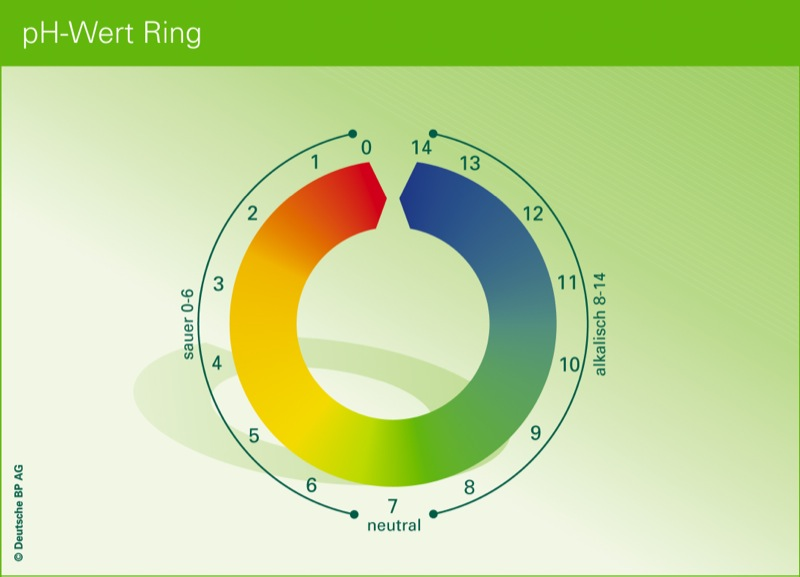
\includegraphics[width=0.618\textwidth]{pictures/phring}
  \caption{PH-Ring}
\end{center}
\end{figure}  
  \begin{enumeratea}
    \item Für Tomaten ist $H=\unitfrac[6.3\cdot10^{-5}]{mol}{l}$,
    für Milch $H=\unitfrac[4\cdot10^{-7}]{mol}{l}$. Berechne
    die zugehörigen \unit{pH}-Werte.
    \item Welcher \unit{pH}-Wert hat eine Lösung mit
    $H=\unitfrac[0]{mol}{l}$?
  \end{enumeratea}
\end{ueb}

\begin{ueb}[Dezibel]\label{dezibel}
  Die Lautstärke $L$ eines Geräuschs von der Intensität $I$ ist
  definiert durch $$L=\unit[10\cdot\log\left(\frac{I}{I_0}\right)]{dB}.$$
  \unit{dB}
  steht für Dezibel, nach dem amerikanischen Ingenieur \textsc{Graham Bell}
  (1847--1922); dem Erfinder des Telefons. $I_0$ bedeutet die Intensität
  eines Geräuschs, das vom menschlichen Ohr gerade noch wahrgenommen
  werden kann.
  \begin{enumeratea}
    \item Die Geräuschintensität normaler Unterhaltung ist etwa eine
    Million mal so gross wie $I_0$. Welchem Dezibel-Wert entspricht
    das?
    \item Eine Intensitätszunahme von $10$ Dezibel empfindet das
    menschliche Ohr als Verdoppelung der Lautstärke. Welcher
    Intensitätszunahme in Prozent entspricht dies?
    \item Ein Düsenflugzeug entwickelt beim Start eine Intensität
    von $10^{13}I_0$. Dezibel-Werte von mehr als $\unit[90]{dB}$
    gelten als gehörschädigend; ist es die angegebene Intensität?
  \end{enumeratea}
\end{ueb}
\begin{figure}
\centering
    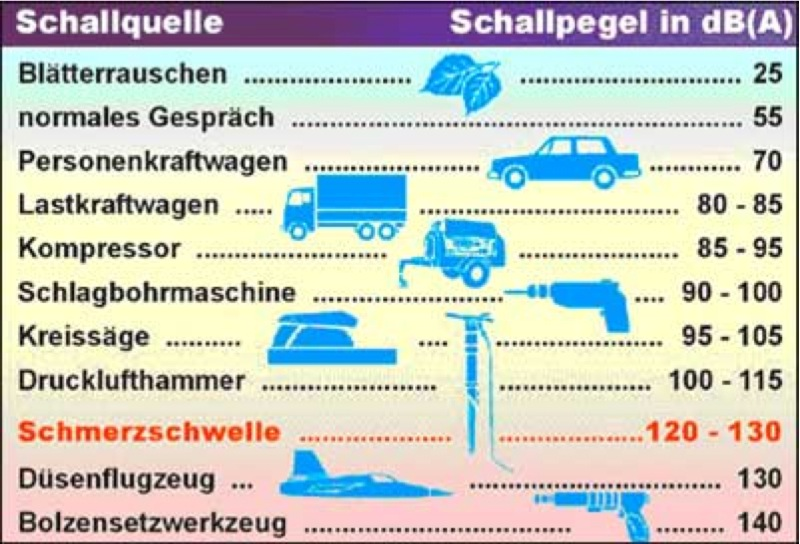
\includegraphics[width=0.618\textwidth]{pictures/dbtabelle}
    \caption{Schallpegel-Tabelle}
 \end{figure}

\begin{ueb}[Richterskala]\label{erdbeben}
Die Stärke von Erdbeben $R$ gibt man durch Werte der sogenannten
    \emph{Richter-Skala} an. Diese ist definiert durch
    $$R=\log\left(\frac{B}{B_0}\right),$$ wobei $B_0$ die Intensität
    eines gerade noch wahrnehmbaren Bebens bezeichnet.

  \begin{enumeratea}
    \item Das Beben von San Francisco im Jahr 1906 hatte eine
    Intensität von $B=B_0\cdot10^{8.25}$. Welchem Wert auf der
    Richter-Skala entspricht dies?
    \item Welche Intensitätsänderung bedeutet eine Zunahme von $1$
    auf der Richterskala?
  \end{enumeratea}  
    \begin{figure}
  \centering
    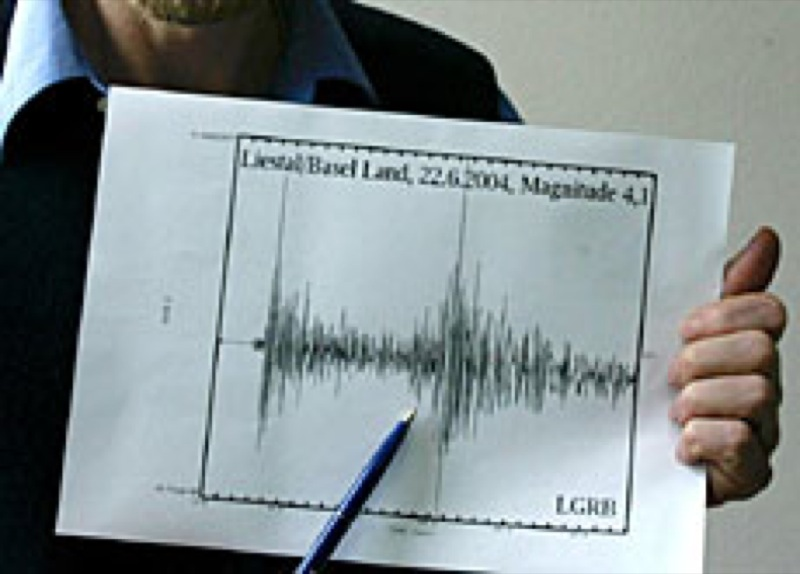
\includegraphics[width=0.618\textwidth]{pictures/erdbebenbasel}\\
    \caption{Aufzeichnung des Erdbebens von Basel vom 22.~Juni 2004}
  \end{figure}
  
\end{ueb}

\subsection{Gleichungen mit Variablen im Exponenten}
Klar, alle Abschnitte dieses Kapitels Logarithmen sind wichtig; aber
dies ist der wichtigste. Die Lösung unseres Ausgangsproblems, die
Bestimmung von Variablen in Exponenten, soll an einem Beispiel
vorgeführt werden.
\begin{bsp}
  Wir lösen die Gleichung $$6^{x-1}=10$$ nach $x$ auf. Dies können
  wir auf zwei Arten tun.
  \begin{enumerate}
    \item Mit Logarithmieren auf beiden Seiten:
    \begin{align}
      \log{6^{x-1}}&=\log{10} \tag{Regel (3)}\\
      (x-1)\cdot\log{6}&= 1 \tag{$\div\log{6}$}\\
      x-1 &= \frac{1}{\log{6}} \tag{$+1$}\\
      x &= \frac{1}{\log{6}} + 1 \approx 2.285 \notag
    \end{align}
    \item Mit der Definition:
    \begin{align}
      6^{x-1}=10\q \Leftrightarrow\q x-1 &= \log_6{10} \tag{Satz \ref{satz:logtr}}\\
      x-1 &= \frac{\log{10}}{\log{6}} \tag{$+1$}\\
      x &= \frac{1}{\log{6}} + 1 \notag
    \end{align}
  \end{enumerate}
  Kontrolle: $$6^{2.285-1} \approx 10 \qq \checkmark$$
\end{bsp}

\begin{ueb}[\glqq Exponentialgleichung\grqq]
  Löse nach $x$ auf: $$2000\cdot1.025^x = 3750$$
\end{ueb}

\begin{ueb}[Homework]
  Stelle drei Gleichungen auf, bei denen die Variable im
  Exponenten vorkommt. Löse diese und überprüfe deine Resultate durch
  Einsetzen in die ursprüngliche Gleichung.
\end{ueb}

\begin{ueb}[Weltbevölkerung]
Nach UNO-Angaben lebten 1988 auf der Erde 5113 Millionen Menschen; die jährliche Wachstumsrate betrug 1.7\%. Wann wird unter der Annahme, dass diese Zuwachsrate konstant bleibt, jedem Menschen nur noch ein Stehplatz von $\unit[\frac{1}{4}]{m^2}$ zur Verfügung stehen? (Die Landfläche beträgt 29\% der Erdoberfläche.)
\end{ueb}

\begin{ueb}[Konsum]
Der Landesindex der Konsumentenpreise betrug im September 1981 94.5 Punkte und im September 1987 109.7 Punkte.
\begin{enumeratea}
\item Berechne den Landesindex im September 1989
unter der Annahme von exponentiellem Wachstum.
\item Wann wird der Landesindex 130 Punkte erreichen?
\end{enumeratea}
\end{ueb}

\begin{ueb}[Spannung]
Die Spannung $U$ (in Volt) einer 12-Volt-Batterie
beträgt während des Einschaltvorganges im Zeitpunkt $t$ (in Sekunden)
$$U(t) = a(1 - b^t)$$
Man misst $U(0.1) = 10.22$.
\begin{enumeratea}
\item Bestimme die Parameter $a$ und $b$.
\item Wie gross ist die Spannung nach $0.2$ Sekunden?
\item Wann beträgt die Spannung 6 Volt?
\end{enumeratea}
\end{ueb}

\begin{ueb}[Zerfall]
Beim radioaktiven Zerfall wird meistens die sogenannte Halbwertszeit angegeben. Die Halbwertszeit ist die Zeit, in der die Hälfte der zu Beginn vorhandenen Atome zerfallen ist.
\begin{enumeratea}
\item Berechne die Halbwertszeit für Strontium 89, für das die Zerfallsfunktion die Form
$$N(t)=N_0\cdot0.98636808^t$$
hat (t in Tagen).
\item Für Uran 239 beträgt die Halbwertszeit $T_{\nicefrac{1}{2}}=23.5$
Minuten. Stelle die Gleichung der Zerfallsfunktion auf, wenn zu Beginn $N_0$ Atome vorhanden sind.
\end{enumeratea}
\end{ueb}

\begin{ueb}[Altersbestimmung]
In lebenden Organismen besteht Kohlenstoff aus stabilen Atomkernen sowie einem Anteil ($3\cdot10^{-8}\%$) aus radioaktiven Atomkernen C$_{14}$, die durch kosmische Strahlung entstehen. Sobald ein organischer Stoff stirbt, nimmt der C$_{14}$-Anteil mit einer Halbwertszeit von 5736 Jahren exponentiell ab.
\begin{enumeratea}
\item Im Jahre 1960 stellte man in der Leinwand einer altägyptischen Königsmumie einen C$_{14}$-Anteil von $1.75\cdot10^{-8}\%$ fest. Datiere auf hundert Jahre genau.
\item 1950 wurde in der Höhle von Lascaux (Frankreich) Holzkohlenreste mit einem C$_{14}$-Anteil von $0.435\cdot10^{-8}\%$ gefunden. Berechne das Alter dieser Holzkohle.
\end{enumeratea}
\end{ueb}

\begin{ueb}[Info]
In der Informationstheorie versteht man unter dem Informationsgehalt $H$ eines Ereignisses mit der Wahrscheinlichkeit $p$ den Logarithmus von $\frac{1}{p}$ zur Basis 2.
$$H = \log_2\frac{1}{p}\q\text{(Einheit: 1 bit)}$$
Welche Wahrscheinlichkeit gehört zum Informationsgehalt $0, 1,0.5,5, 10.2$ bit?

Eine Münze wird viermal geworfen. Berechne den Informationsgehalt der Ereignisse
\begin{enumeratea}
\item nie Kopf,
\item genau einmal Kopf,
\item genau zweimal Kopf,
\item genau dreimal Kopf
\item viermal Kopf.
\end{enumeratea}
\end{ueb}

\subsection{Die Euler'sche Zahl}
Die geeignetste Basis für eine Exponentialfunktion
$$f(x)=b^x$$
ist die Zahl $\mathrm{e}$, eine Zahl, die in vielen Anwendungen vorkommt. Der Buchstabe $\mathrm{e}$ wurde zu Ehren des in Riehen geborenen Mathematikers \textsc{Leonhard Euler} (1707-1783) gewählt. Wie $\pi$ ist die Euler'sche Zahl irrational, und ihre Dezimaldarstellung beginnt mit
$$\mathrm{e}  =  2.71828182845904523536028747135266\dots$$

\begin{figure}
\begin{center}
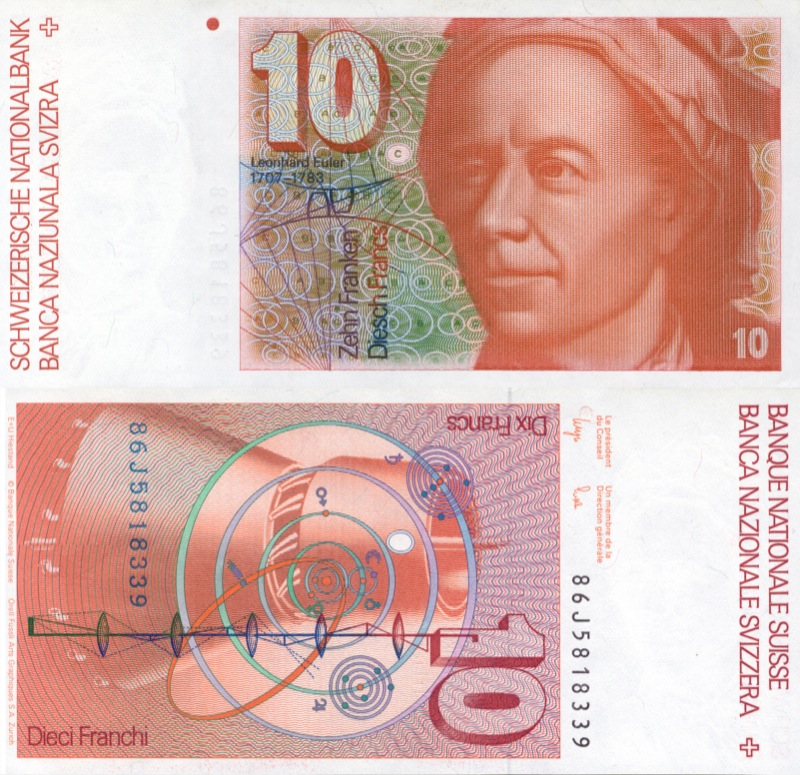
\includegraphics[width=0.618\textwidth]{pictures/euler}
\end{center}
\caption{10-Franken Note alter Serie: Leonard Euler}
\end{figure}

Was es mit der Zahl $e$ auf sich hat, können wir an dieser Stelle nur zu einem kleinen Teil erfahren, denn ihre Bedeutung wird erst nach und nach mit fortschreitendem Stoff klarer werden. Eine Möglichkeit, die Zahl $\mathrm{e}$ kurz und bündig zu charakterisieren, ist diese:
\begin{quote}
$\mathrm{e}$ ist die einzige positive Zahl, für die
$$\mathrm{e}^x\geq1+x\q\forall x\in\mR$$
\end{quote}

\begin{ueb}[guckst du!]
Zeichne mit dem TR $\mathrm{e}^x$ und $x+1$.
\end{ueb}

\begin{ueb}[eingeklemmt]
Zeichne mit dem TR $\mathrm{e}^x$, $2^x$ und $3^x$ und betrachte einen kleinen Ausschnitt um $\point{0}{1}$.
\end{ueb}

Eine weitere schöne Eigenschaft ist folgende.
\begin{bem}
Alle Exponentialfunktionen $b^x$ schneiden die $y$-Achse im Punkt $\point{0}{1}$. Sucht man für eine Exponentialfunktion $b^x$ eine Basis $b$ so, dass die Steigung des Graphen beim Schnittpunkt mit der $y$-Achse exakt $45^\circ$, also $1$, beträgt, dann folgt $b=\mathrm{e}$.
\end{bem}

Obwohl die bisherige Argumentation von einem strengen mathematischen Gesichtspunkt aus betrachtet ein bisschen zu schlampig ist, geben wir uns mit ihr zufrieden. Auch ein genauerer Beweis liefert dasselbe Resultat.

Um die Basis Euler'sche Zahl zu berechnen, gehen wir folgendermassen vor: Wir wählen ein positives $x$ und betrachten jene Basis $b$, für die
$$b^x=1+x$$
oder, nach $b$ aufgelöst
$$b=(1+x)^{\frac{1}{x}}$$
ist. Dies ist genau jene Basis, für die der Graph von $b^x$ die Gerade $1+x$ in einem Punkt mit der (positiven) x-Koordinate $x$ schneidet. Wenn wir nun $x$ immer kleiner machen ($x\to0$), wird $b$ immer näher an $\mathrm{e}$ heran rücken.
Wir berechnen sinngemäss
$$\left(1+\frac{1}{n}\right)^n$$
für grosse natürliche Zahlen $n$, also $n\to\infty$.

\begin{table}
\begin{center}
\scalebox{1.1}{
\begin{tabular}{|c|c|}
\hline
\rowcolor{lightyellow}\spaltenheight    $n$ & $\left(1+\frac{1}{n}\right)^n$\spaltensep\hline\hline
\rowcolor{Gray}\spaltenheight 1 & 2\spaltensep\hline
\rowcolor{lightyellow}\spaltenheight    2 & 2.25\spaltensep\hline
\rowcolor{Gray}\spaltenheight 10 & 2.59\dots\spaltensep\hline
\rowcolor{lightyellow}\spaltenheight    100 & 2.70\dots\spaltensep\hline
\rowcolor{Gray}\spaltenheight 1000 & 2.716\dots\spaltensep\hline
\rowcolor{lightyellow}\spaltenheight    100000 & 2.71826\dots\spaltensep\hline
\rowcolor{Gray}\spaltenheight 100000000 & 2.71828\dots\spaltensep\hline
\end{tabular}
}
\end{center}
\caption{Approximation an $\mathrm{e}$}
\end{table}

\begin{cdef}[Euler'sche Zahl]{}
Es
\marginnote{
\qrcode{
https://www.youtube.com/watch?v=0NK4BMpqd2Q}
}
ist denkbar, als Definition für die Euler'sche Zahl
$$\mathrm{e}:=\lim_{n\to\infty}\left(1+\frac{1}{n}\right)^n=2.718281828\dots$$
zu verwenden.
\end{cdef}

\begin{cdef}[Natürliche Exponentialfunktion und logarithmus naturalis]{}
Die entsprechende Exponentialfunktion
$$\mathrm{exp}(x)=\mathrm{e}^x$$
bezeichnet man als die \emph{natürliche Exponentialfunktion}.

Die entsprechende Logarithmusfunktion, also die Umkehrfunktion von $x\mapsto \mathrm{e}^x$, wird \emph{natürliche Logarithmusfunktion} genannt:
$$\mathrm{exp}^{-1}(x)=\log_\mathrm{e}(x)=:\ln(x)$$
\end{cdef}

\begin{bem}
Der Taschenrechner stellt mit speziellen Tasten sowohl die Funktionswerte $\mathrm{e}^x$ als auch die Funktionswerte $\ln(x)$ zur Verfügung.
\end{bem}

\begin{bem}
Fortgeschrittene Rechner verwenden selbstverständlich als Basis einer Exponentialfunktion $\mathrm{e}$ und bezeichnen den $\ln$ oft als $\log$.

Später werden wir in erster Linie nur noch diese beiden Funktionen verwenden, da sich alle anderen Exponential- und Logarithmusfunktionen auf diese beiden Funktionen zurückführen lassen. Diese schöne Tatsache wollen wir mit den beiden nächsten Übungen untermauern.
\end{bem}

\begin{ueb}[umschreiben]
Stelle die Exponentialfunktion $f(x)=3.5\cdot2^x$ als natürliche Exponentialfunktion der Form
$$f(x)=a\cdot \mathrm{e}^{cx}$$
dar.
\end{ueb}

\begin{ueb}[Es gibt nur eine Basis\dots]
Überlege dir, dass jede Exponentialfunktion $f(t)=a\cdot b^t$
sich in die Form
$$f(t)=d\cdot \mathrm{e}^{ct}$$
umwandeln lässt.

Finde eine Formel für die Parameter $c$ und $d$ bei der natürlichen Exponentialfunktion, wenn die Parameter $a$ und $b$ gegeben sind.
\end{ueb}

\begin{ueb}[Epidemie]
Für die Zeit während der Ausbreitung einer Epidemie kann man die Anzahl der nach $t$ Tagen infizierten Individuen durch die folgende Modellfunktion angeben:
$$N(t)=\frac{M}{1+c\mathrm{e}^{-at}}$$
Für eine bestimmte Epidemie seien $M= 1000$, $c=999$
und $a=0.4$.
\begin{enumeratea}
\item Wie viele Individuen sind nach 0, 10, 20, 30 Tagen infiziert?
\item Nach wie vielen Tagen sind 200, 500, 950 Individuen infiziert?
\item Zeichne den Graphen der Funktion.
\end{enumeratea}
\end{ueb}

\begin{ueb}[Forellen]
In einer Forellenzuchtanstalt wurde bei gleichartigen Forellen die jeweils nach $t$ Monaten erreichte durchschnittliche Länge $\unit[L]{cm}$ gemessen. Aus den Messungen ergab sich das \glqq Wachstumsgesetz\grqq:
$$L(t) =25(1- \mathrm{e}^{-0.25t})$$
\begin{enumeratea}
\item Berechne die Länge nach 0, 4, 8 Monaten.
\item Wann waren die Forellen etwa $\unit[10,20]{cm}$ lang?
Wann werden sie $\unit[25]{cm}$ lang sein?
\end{enumeratea}
\end{ueb}

\cleardoublepage

\appendix

\section{Relationen}
\begin{wrapfigure}{r}{0.382\textwidth}
  \begin{center}
    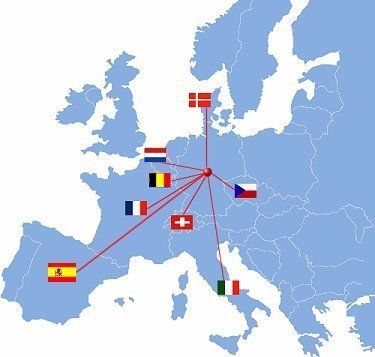
\includegraphics[width=0.382\textwidth]{pictures/relationen}
  \end{center}
%\caption{You Know my Name}
\end{wrapfigure}
Personen oder auch Dinge stehen oft in Beziehung. Es gibt verwandtschaftliche oder freundschaftliche Beziehungen. Es gibt Beziehungen von Menschen zu ihrer Heimat, von Eigent\"umern zu ihrem Besitztum, oder auch zwischen Konjunktur und Arbeitslosigkeit, zwischen Qualit\"at und Preis etc.

Manche Beziehungen lassen sich graphisch darstellen und mathematisch beschreiben. Im Folgenden werden Menge und Beziehungen zwischen ihren Elementen betrachtet.
\begin{bsp}
Es gibt eine Beziehung, in der Mathematik sagt man \emph{Relation}, zwischen den Mitgliedern dieser Klasse und den m\"oglichen Freif\"achern, welche Angeboten werden.
\end{bsp}
\begin{bem}
Unter einer Relation $R$ zwischen den Elementen der Mengen $\mA$ und $\mB$ versteht man eine beliebige Beziehung (Zuordnung), wodurch jedem Element $x\in\mA$ \emph{kein, genau ein} oder \emph{mehr als ein} Element $y\in\mB$ zugeordnet wird. Man schreibt
$$R:\mA\longrightarrow\mB$$
\end{bem}
\begin{bsp}
Im obigen Beispiel steht $R$ f\"ur \glqq zu einem Klassenmitglied das Freifach zuordnen\grqq, $\mA$ f\"ur die Menge der Sch\"ulerinnen und Sch\"uler der Klasse und $\mB$ f\"ur die Menge der angebotenen Freif\"acher.
\end{bsp}
\begin{bem}
Offensichtlich kann jede Relation als Menge von geordneten Paaren $\point{x}{y}$ notiert werden. Um eine Relation via Mengenlehre zu definieren brauchen wir noch folgende
\begin{cdef}[Produktmenge]{}
Die \emph{Produktmenge} zweier Mengen $\mA$ und $\mB$ ist die Menge aller geordneten Paare $\point{a}{b}$, wobei $a\in\mA$ und $b\in\mB$ ist. Man schreibt
$$\mA\times\mB=\setm{\point{a}{b}}{a\in\mA\text{ und }b\in\mB}.$$
\end{cdef}
Damit l\"asst sich der Relationsbegriff auch rein mengentheoretisch definieren. Wir betrachten zuerst noch ein Beispiel zur Produktmenge.
\begin{bsp}
$\mR\times\mR$, kurz $\mR^2$, ist die Menge aller Punkte einer Ebene. Die Paare $\point{x}{y}$ k\"onnen als Punkte in einem rechtwinkligen Koordinatensystem veranschaulicht werden.
\end{bsp}
\begin{ueb}
Beschreibe die Menge $\mR^3$. Welche Form/Schreibweise hat ein Punkt in dieser Menge?
\end{ueb}
\end{bem}
\begin{cdef}[Relatio]{}
Eine \emph{Relation} $R$
\marginnote{
\qrcode{
https://www.youtube.com/watch?v=GBhMplA6--4}
}
zwischen den Elementen der Mengen $\mA$ und $\mB$ ist eine Teilmenge der Produktmenge $\mA\times\mB$.
\end{cdef}
\begin{bem}
Die Darstellung der Relationen in einem rechtwinkligen Koordinatensystem nennt man den Graphen der Relation.
\end{bem}

F\"ur die folgenden \"Ubungen erinnern wir uns an die Definition des Betrags:
\begin{cdef}[Betrag]{}
F\"ur jede reelle Zahl $x$ ist der \emph{Betrag} von $x$ definiert durch
$$\abs{x}\;=
\begin{cases}
\phantom{-}x\q\text{falls }x\geq0\\
-x\q\text{falls }x<0
\end{cases}$$
\end{cdef}

\begin{ueb}
Beachte, dass $x$ und $y$ als reelle Zahlen zu betrachten sind, falls keine andere Vereinbarung vorliegt. Zeichne den Graphen der Relation
\begin{enumeratea}
\item $R=\setm{\point{x}{y}}{y\leq x}$
\item $R=\setm{\point{x}{y}}{x<2\text{ und }y<4, x,y\in\mZ}$
\item $R=\setm{\point{x}{y}}{\abs{x}\leq5}$
\item $R=\setm{\point{x}{y}}{\abs{y}>3}$
\item $R=\setm{\point{x}{y}}{\abs{x}+\abs{y}\leq4}$
\end{enumeratea}
\end{ueb}

\begin{ueb}
Wie lautet die Relation, die durch den folgenden Graphen veranschaulicht wird?
\begin{center}
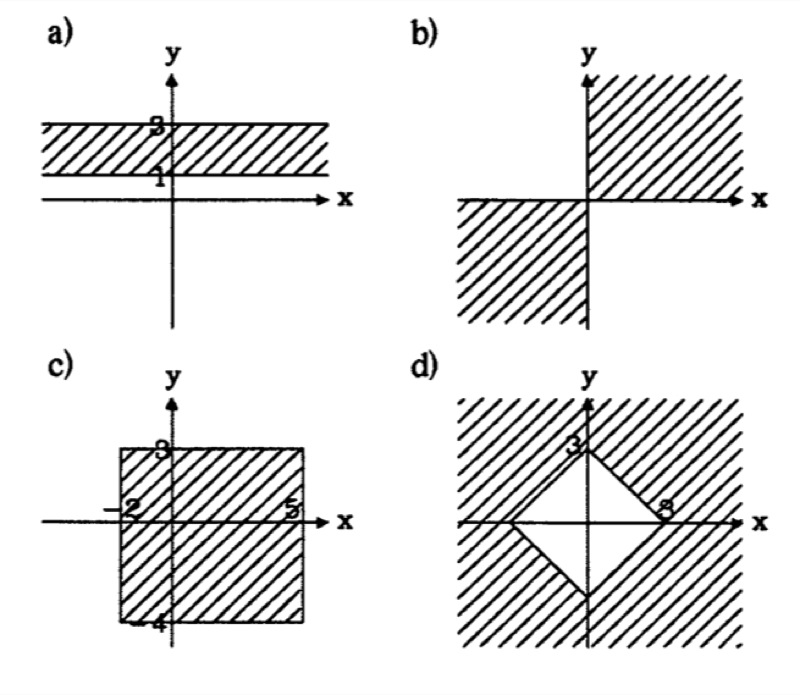
\includegraphics[width=0.618\textwidth]{pictures/relation}
\end{center}
\end{ueb}

\section{Abbildungen}
\begin{wrapfigure}{r}{0.382\textwidth}
  \begin{center}
    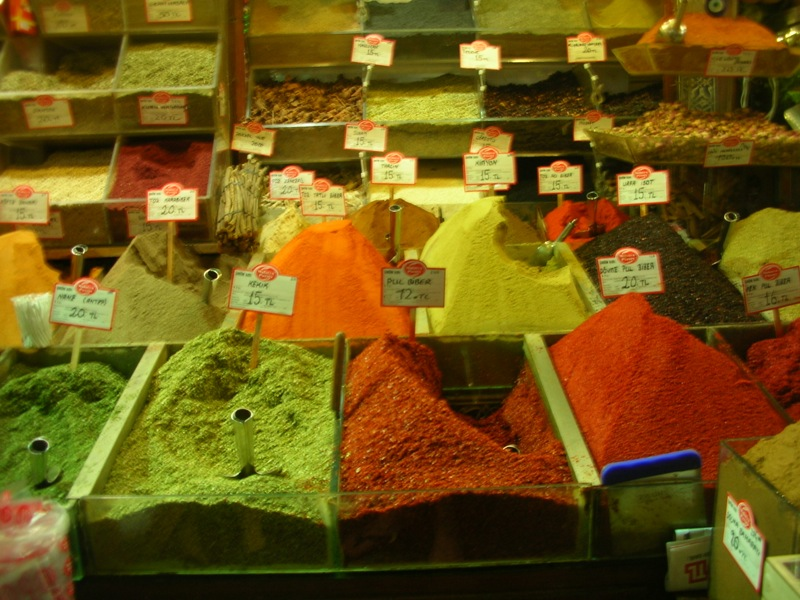
\includegraphics[width=0.382\textwidth]{pictures/gewuerze}
  \end{center}
%\caption{You Know my Name}
\end{wrapfigure}
In manchen L\"andern ist der Preis einer Ware oft nicht eindeutig festgelegt. Dem einen macht das Handeln zwar Spass, dem andern w\"are es aber lieber, wenn die Relation zwischen Ware und Preis einer eindeutigen Zuordnung entspricht. Ist eine Relation n\"amlich nicht eindeutig festgelegt, so k\"onnen Missverst\"andnisse auftreten.

Verlagsh\"auser und Buchh\"andler haben die ISBN (Internationale Standardbuchnummer) eingef\"uhrt, um Missverst\"andnisse auszuschalten. Durch die ISBN ist jedem Buch $x$ genau eine Buchnummer $y$ zugeordnet. In der Mathematik spielen die Relationen, die sich auf die gesamte Ausgangsmenge beziehen und eine eindeutige Zuordnung schaffen, eine besonders wichtige Rolle.

\begin{cdef}[Abbildung]{}
Eine \emph{Abbildung} $f$ von einer Ausgangsmenge $\mA$ in eine Zielmenge $\mB$ ist eine Relation, die jedem Element $x\in\mA$ \emph{genau ein} Element $y\in\mB$ zuordnet. Man schreibt
$$f:\mA\longrightarrow\mB$$
oder f\"ur Elemente
$$y=f(x).$$
\end{cdef}
Man nennt $y$ das \emph{Bild} von $x$, $x$ das \emph{Urbild} von $y$.
\begin{bem}
Jede Abbildung ist eine Relation, aber nicht jede Relation eine Abbildung.
\end{bem}
\begin{ueb}[geometrische Abbildungen]
Nenne vier geometrische Abbildungen und \"uber\-le\-ge dir, warum der Name Abbildung gerechtfertigt ist.
\end{ueb}

\section{Biquadratische Gleichungen}

\begin{cdef}[Biquadratische Gleichung]{}
Gleichungen, in denen die Variable nur in der zweiten und vierten Potenz vorkommt, nennt man \emph{biquadratisch}.  
\end{cdef}

\begin{bsp}
Die Gleichung
$$2x^4-3x^2-20=0$$
ist biquadratisch.
\end{bsp}
Solche Gleichungen sind wegen $x^4=(x^2)^2$ mit den Methoden zur L\"osung von quadratischen Gleichungen l\"osbar. Man reduziert durch eine Substitution die biquadratische Gleichung auf eine quadratische und l\"ost diese. Danach bleiben noch quadratische Gleichungen \"ubrig, die einfach gel\"ost werden k\"onnen.

Wir \emph{substituieren} in der Gleichung aus dem Beispiel die biquadratische Variable, d.h. wir setzen
$$x^2=z$$
und erhalten
$$2z^2-3z-20=0.$$
Nun k\"onnen wir einfach nach $z$ l\"osen, was
$$z_1=-2.5\q\text{und}\q z_2=4$$
liefert. Da $x^2=z$ haben wir noch die L\"osungen von
$$-2.5=x^2\q\text{und}\q 4=x^2$$
zu bestimmen. Die erste Gleichung hat keine L\"osung in $\mR$ und die zweite liefert
$$x_1=2\q\text{und}\q x_2=-2.$$
Nat\"urlich kann man das Verfahren der Substitution auch auf h\"oher gradige Gleichungen anwenden.

\begin{ueb}
Wie viele L\"osungen kann eine biquadratische Gleichung haben?
\end{ueb}

\begin{ueb}
Gib je eine biquadratische Gleichung mit keiner, einer, zwei, drei und eine mit vier L\"osungen.
\end{ueb}

\begin{ueb}
Bestimme alle L\"osungen der Gleichung
$$x^4-13x^2=-36.$$
\end{ueb}

\begin{ueb}
Bestimme alle L\"osungen der Gleichung
$$(x^2+4)^2-25(x^2+4)+100=0.$$
\end{ueb}

\section{L\"osungsstrategien für Gleichungen}

Abschliessend
    \marginnote{
\qrcode{
https://www.youtube.com/watch?v=yci4Bc5EKbY}
}
zu den quadratischen Funktionen möchte ich bemerken, dass man nun die gängigen Mittel zum Lösen von Gleichungen der Mittelschulmathematik kennt. Nebst linearen Gleichungen trifft man auch auf solche, bei denen die Variable im Nenner auftaucht, auf Wurzelgleichungen (die auf lineare oder quadratische zurückgeführt werden können) oder eben auf quadratische bzw.  Gleichungen. Das heisst, es ist nützlich, wenn man eine Art Schema zur Analyse das vorliegenden Gleichungstyps parat hat. Damit kann man nach Analyse die passende Lösungsstrategie wählen.

\begin{landscape}
\begin{figure}
\begin{center}

% Define block styles
%\tikzstyle{block} = [rectangle, draw, fill=blue!20, text width=5em, text centered, rounded corners, minimum height=4em]
\tikzstyle{block} = [rectangle, draw, fill=blue!20!red!10!, node distance=15ex, text centered, %rounded corners,
text width=25ex, minimum height=6ex
]
\tikzstyle{block2} = [rectangle, draw, fill=blue!10!green!40, node distance=15ex, text centered, rounded corners, minimum height=4ex]

\scalebox{0.9}{
\begin{tikzpicture}[level distance=3cm, level 1/.style={sibling distance=4cm}, level 2/.style={sibling distance=2.6cm}, level 3/.style={sibling distance=2.7cm}, every node/.style={draw, rectangle, minimum width=1cm}]
\node [block] (glstart) {Gleichung}
child {node {linear}
    child {node [block2] {Standardlösung}
    }
}
child {node {quadratisch}
    child {node [block2] {rein}}
    child {node {mit $x$}
        child {node [block2] {faktorisieren}}
        child {node [block2]{Lösungsformel}}
    }
}
child {node {unter Wurzel}
    child {node (root) {quadrieren}}
}
child {node {im Nenner}
    child {node (nenner) {mit Variable multiplizieren}}
};
\draw[->] (root) -- ++(1.4,0) |- (glstart);
\draw[->] (nenner) -- ++(2.7,0) |- (glstart);
\end{tikzpicture}
}
\end{center}
\caption{Vorgehen beim Lösen von Gleichungen}
\end{figure}
\end{landscape}

\section{Funktionsverwandtschaften}

\subsection{Einleitung}
  In diesem Abschnitt wollen wir uns Funktionen anschauen, welche insofern miteinander verwandt sind, als dass deren Graphen durch eine Translation, eine Streckung oder eine Drehung ineinander übergeführt werden können. Es geht darum, allgemeine Aussagen über die Ähnlichkeit ihrer Funktionsgleichungen machen zu können, wenn ihre Graphen kongruent sind; und vice versa. Eine Anwendung ist:
  \begin{ueb}
  Die Osterhasen stehen bald wieder in den Regalen; lecker! Für deren Produktion hat ein Betrieb Fixkosten von $\unit[10'000]{CHF}$ und Kosten pro Hase von $\unit[0.50]{CHF}$. Stelle die Kostenfunktion $k(x)$ auf, welche die Produktionskosten $k$ in Abhängigkeit der Anzahl produzierten Osterhasen $x$ angibt. Wähle eine geeignete Skala für Ihr Koordinatensystem und zeichne den Graphen.\\
Aufgrund unvorhergesehener Probleme bei der Produktion steigen die Fixkosten um $\unit[25]{\%}$. Bestimme die angepasste Kostenfunktion $k_a(x)$ und zeichne deren Graphen.

\begin{ueb}
Zeichne die Graphen von $f(x)=x^2$, $g(x)=(x-2)^2$ und $h(x)=(x+3)^2$ in ein und das selbe Koordinatensystem.
\end{ueb}
\begin{ueb}
Zeichne die Graphen von $f(x)=\log(x)$, $g(x)=\log(x+1)$ und $h(x)=1+\log(x)$ in ein und das selbe Koordinatensystem.
\end{ueb}
\begin{ueb}
Zeichne die Graphen von $f(x)=x^2$, $g(x)=(x+1)^2-2$ und $h(x)=(x-2)^2+1$ in ein und das selbe Koordinatensystem.
\end{ueb}
\begin{ueb}
Zeichne die Graphen von $f(x)=2^x$, $g(x)=2^{x-1}$ und $h(x)=\frac{1}{2}2^x$ in ein und das selbe Koordinatensystem.
\end{ueb}
\end{ueb}

\subsection{Untersuchung der Verwandtschaften}
  \begin{bsp}
  Wir betrachten den Graphen einer beliebigen Funktion $y=f(x)$. Wie sieht der Graph der Funktion $g(x)$ aus, der aus dem Graphen von $f$ entsteht, indem man letzteren um $1$ in $y$-Richtung verschiebt? Wie lautet die Funktionsgleichung von $g$?\\[-1ex]

\begin{center}
\begin{tikzpicture}[line cap=round,line join=round,>=triangle 45,x=0.5cm,y=0.5cm]
\draw[->,color=black] (-2.52,0) -- (11.1,0);
\foreach \x in {-2,-1,1,2,3,4,5,6,7,8,9,10}
\draw[shift={(\x,0)},color=black] (0pt,2pt) -- (0pt,-2pt);
\draw[color=black] (10.76,0.08) node [anchor=south west] { x};
\draw[->,color=black] (0,-3.1) -- (0,4.66);
\foreach \y in {-3,-2,-1,1,2,3,4}
\draw[shift={(0,\y)},color=black] (2pt,0pt) -- (-2pt,0pt);
\draw[color=black] (0.1,4.26) node [anchor=west] { y};
\clip(-2.52,-3.1) rectangle (11.1,4.66);
\draw[line width=2pt, smooth,samples=100,domain=-2.0:1.0] plot(\x,{0});
\draw[line width=2pt, smooth,samples=100,domain=1.0:3.0] plot(\x,{\x-1});
\draw[line width=2pt, smooth,samples=100,domain=3.0:7.0] plot(\x,{0-(0.5)*\x+3.5});
\draw[line width=2pt, smooth,samples=100,domain=7.0:10.0] plot(\x,{0});
\draw (1.3,1.9) node[anchor=north west] {$f$};
\end{tikzpicture}
\end{center}
\end{bsp}

\subsubsection{Verschiebung in y-Richtung}
Wir verschieben den Graphen von $f$ um $1$ in $y$-Richtung und erhalten folgendes Bild:\\

\definecolor{wwqqqq}{rgb}{0.4,0,0}
\begin{center}
\scalebox{0.8}{
\begin{tikzpicture}[line cap=round,line join=round,>=triangle 45,x=0.5cm,y=0.5cm]
\draw[->,color=black] (-2.52,0) -- (11.1,0);
\foreach \x in {-2,-1,1,2,3,4,5,6,7,8,9,10,11}
\draw[shift={(\x,0)},color=black] (0pt,2pt) -- (0pt,-2pt);
\draw[color=black] (10.76,0.08) node [anchor=south west] { x};
\draw[->,color=black] (0,-3.1) -- (0,4.66);
\foreach \y in {-3,-2,-1,1,2,3,4}
\draw[shift={(0,\y)},color=black] (2pt,0pt) -- (-2pt,0pt);
\draw[color=black] (0.1,4.26) node [anchor=west] { y};
\clip(-2.52,-3.1) rectangle (11.1,4.66);
\draw[line width=2pt, smooth,samples=100,domain=-2.0:1.0] plot(\x,{0});
\draw[line width=2pt, smooth,samples=100,domain=1.0:3.0] plot(\x,{\x-1});
\draw[line width=2pt, smooth,samples=100,domain=3.0:7.0] plot(\x,{0-(0.5)*\x+3.5});
\draw[line width=2pt, smooth,samples=100,domain=7.0:10.0] plot(\x,{0});
\draw (1.3,1.7) node[anchor=north west] {$f$};
\draw[line width=1.6pt,dash pattern=on 3pt off 3pt,color=wwqqqq, smooth,samples=100,domain=-2.0:1.0] plot(\x,{1});
\draw[line width=1.6pt,dash pattern=on 3pt off 3pt,color=wwqqqq, smooth,samples=100,domain=1.0:3.0] plot(\x,{\x});
\draw[line width=1.6pt,dash pattern=on 3pt off 3pt,color=wwqqqq, smooth,samples=100,domain=3.0:7.0] plot(\x,{0-(0.5)*\x+4.5});
\draw[line width=1.6pt,dash pattern=on 3pt off 3pt,color=wwqqqq, smooth,samples=100,domain=7.0:10.0] plot(\x,{1});
\draw (1.2,2.6) node[anchor=north west] {$g$};
\end{tikzpicture}
}
\end{center}

Wegen der Verschiebung um $1$ in $y$-Richtung ist jeder Wert von $g(x)$ um $1$ grösser als der entsprechende Wert von $f(x)$. Deshalb ist $g(x)=f(x)+1$.

Allgemein kann man also sagen, dass der Graph von $f(x)+a$ aus dem Graphen von $f(x)$ durch eine Verschiebung parallel zur $y$-Achse um den Wert $a$ hervorgeht.

\subsubsection{Verschiebung in x-Richtung}
Verschiebe den Graphen von $f$ um $1$ in $x$-Richtung und zeichne ihn. Wie lautet die Funktionsgleichung $g(x)$ des neuen Graphen? Formuliere eine Verschiebung in $x$-Richtung um den Wert $a$ allgemein.\\[2ex]

\begin{center}
\begin{tikzpicture}[line cap=round,line join=round,>=triangle 45,x=0.5cm,y=0.5cm]
\draw[->,color=black] (-2.52,0) -- (11.1,0);
\foreach \x in {-2,-1,1,2,3,4,5,6,7,8,9,10}
\draw[shift={(\x,0)},color=black] (0pt,2pt) -- (0pt,-2pt);
\draw[color=black] (10.76,0.08) node [anchor=south west] { x};
\draw[->,color=black] (0,-3.1) -- (0,4.66);
\foreach \y in {-3,-2,-1,1,2,3,4}
\draw[shift={(0,\y)},color=black] (2pt,0pt) -- (-2pt,0pt);
\draw[color=black] (0.1,4.26) node [anchor=west] { y};
\clip(-2.52,-3.1) rectangle (11.1,4.66);
\draw[line width=2pt, smooth,samples=100,domain=-2.0:1.0] plot(\x,{0});
\draw[line width=2pt, smooth,samples=100,domain=1.0:3.0] plot(\x,{\x-1});
\draw[line width=2pt, smooth,samples=100,domain=3.0:7.0] plot(\x,{0-(0.5)*\x+3.5});
\draw[line width=2pt, smooth,samples=100,domain=7.0:10.0] plot(\x,{0});
\draw (1.3,1.9) node[anchor=north west] {$f$};
\end{tikzpicture}
\end{center}
  
\subsubsection{Einschub}
 Für das Folgende ist es praktisch, den Begriff der affinen Abbildung einzuführen.
 \begin{cdef}[Affinität]{}
 Eine Abbildung (Funktion/Translation) heisst \emph{affin}, wenn die Verbindungsgeraden Ausgangspunkt $P$ -- Bildpunkt $P'$ alle parallel sind. Die Richtung dieser Parallelen heisst \emph{Affinitätsrichtung}.
 \end{cdef}
 \begin{csatz}[Linearität der Affinität]{}
 Der Abstand eines Bildpunktes von einer festen Geraden (der sogenannten \emph{Affinitätsachse}) beträgt das $k$-fache des Abstandes des Ausgangspunktes von dieser Geraden, wobei $k\in\D{R}$. $k$ heisst \emph{Affinitätsfaktor}.
 \end{csatz}
 \begin{bsp}
 Betrachte den Graphen der Funktion $f(x)=x^2$ auf deinem TR. Anschliessend lässt du zusätzlich den Graphen von $g(x)=\frac{1}{2}x^2$ von deinem TR zeichnen. Die Translation, welche den Graphen von $f$ in $g$ überführt ist eine affine Abbildung mit Affinitätsfaktor $k=\frac{1}{2}$ und hat als Affinitätsachse die $x$-Achse. Die Affinitätsrichtung ist parallel zur $y$-Achse.
 \end{bsp}
  
\subsubsection{Streckung in y-Richtung}
Bilde den Graphen von $f$ affin in $y$-Richtung ab, wobei du als Affinitätsachse die $x$-Achse wählst und $k=2$. Wie lautet die Funktionsgleichung $g(x)$?\\[3ex]

\begin{center}
\begin{tikzpicture}[line cap=round,line join=round,>=triangle 45,x=0.5cm,y=0.5cm]
\draw[->,color=black] (-2.52,0) -- (11.1,0);
\foreach \x in {-2,-1,1,2,3,4,5,6,7,8,9,10}
\draw[shift={(\x,0)},color=black] (0pt,2pt) -- (0pt,-2pt);
\draw[color=black] (10.76,0.08) node [anchor=south west] { x};
\draw[->,color=black] (0,-3.1) -- (0,4.66);
\foreach \y in {-3,-2,-1,1,2,3,4}
\draw[shift={(0,\y)},color=black] (2pt,0pt) -- (-2pt,0pt);
\draw[color=black] (0.1,4.26) node [anchor=west] { y};
\clip(-2.52,-3.1) rectangle (11.1,4.66);
\draw[line width=2pt, smooth,samples=100,domain=-2.0:1.0] plot(\x,{0});
\draw[line width=2pt, smooth,samples=100,domain=1.0:3.0] plot(\x,{\x-1});
\draw[line width=2pt, smooth,samples=100,domain=3.0:7.0] plot(\x,{0-(0.5)*\x+3.5});
\draw[line width=2pt, smooth,samples=100,domain=7.0:10.0] plot(\x,{0});
\draw (1.3,1.9) node[anchor=north west] {$f$};
\end{tikzpicture}
\end{center}
  
\subsubsection{Streckung in x-Richtung}
Zeichne den Graphen von $g(x)=f(2x)$. Bestimme Affinitätsachse, Affinitätsrichtung und Affinitätsfaktor dieser Translation, die den Graphen von $f$ in denjenigen von $g$ überführt.\\[3ex]

\begin{center}
\begin{tikzpicture}[line cap=round,line join=round,>=triangle 45,x=0.5cm,y=0.5cm]
\draw[->,color=black] (-2.52,0) -- (11.1,0);
\foreach \x in {-2,-1,1,2,3,4,5,6,7,8,9,10}
\draw[shift={(\x,0)},color=black] (0pt,2pt) -- (0pt,-2pt);
\draw[color=black] (10.76,0.08) node [anchor=south west] { x};
\draw[->,color=black] (0,-3.1) -- (0,4.66);
\foreach \y in {-3,-2,-1,1,2,3,4}
\draw[shift={(0,\y)},color=black] (2pt,0pt) -- (-2pt,0pt);
\draw[color=black] (0.1,4.26) node [anchor=west] { y};
\clip(-2.52,-3.1) rectangle (11.1,4.66);
\draw[line width=2pt, smooth,samples=100,domain=-2.0:1.0] plot(\x,{0});
\draw[line width=2pt, smooth,samples=100,domain=1.0:3.0] plot(\x,{\x-1});
\draw[line width=2pt, smooth,samples=100,domain=3.0:7.0] plot(\x,{0-(0.5)*\x+3.5});
\draw[line width=2pt, smooth,samples=100,domain=7.0:10.0] plot(\x,{0});
\draw (1.3,1.9) node[anchor=north west] {$f$};
\end{tikzpicture}
\end{center}
  
\subsubsection{Spiegelung an der x-Achse}
Zeichne den Graphen von $g$, welcher durch Spiegelung des Graphen von $f$ an der $x$-Achse entsteht, und bestimme die Funktionsgleichung von $g$. Gib anschliessend an, um welche affine Abbildung es sich hierbei handelt.\\[3ex]

\begin{center}
\begin{tikzpicture}[line cap=round,line join=round,>=triangle 45,x=0.5cm,y=0.5cm]
\draw[->,color=black] (-2.52,0) -- (11.1,0);
\foreach \x in {-2,-1,1,2,3,4,5,6,7,8,9,10}
\draw[shift={(\x,0)},color=black] (0pt,2pt) -- (0pt,-2pt);
\draw[color=black] (10.76,0.08) node [anchor=south west] { x};
\draw[->,color=black] (0,-3.1) -- (0,4.66);
\foreach \y in {-3,-2,-1,1,2,3,4}
\draw[shift={(0,\y)},color=black] (2pt,0pt) -- (-2pt,0pt);
\draw[color=black] (0.1,4.26) node [anchor=west] { y};
\clip(-2.52,-3.1) rectangle (11.1,4.66);
\draw[line width=2pt, smooth,samples=100,domain=-2.0:1.0] plot(\x,{0});
\draw[line width=2pt, smooth,samples=100,domain=1.0:3.0] plot(\x,{\x-1});
\draw[line width=2pt, smooth,samples=100,domain=3.0:7.0] plot(\x,{0-(0.5)*\x+3.5});
\draw[line width=2pt, smooth,samples=100,domain=7.0:10.0] plot(\x,{0});
\draw (1.3,1.9) node[anchor=north west] {$f$};
\end{tikzpicture}
\end{center}
  
\subsubsection{Spiegelung an der y-Achse}
Zeichne den Graphen von $g$, welcher durch Spiegelung des Graphen von $f$ an der $y$-Achse entsteht, und bestimme die Funktionsgleichung von $g$. Gib anschliessend an, um welche affine Abbildung es sich hierbei handelt.\\[3ex]

\begin{center}
\begin{tikzpicture}[line cap=round,line join=round,>=triangle 45,x=0.5cm,y=0.5cm]
\draw[->,color=black] (-2.52,0) -- (11.1,0);
\foreach \x in {-2,-1,1,2,3,4,5,6,7,8,9,10}
\draw[shift={(\x,0)},color=black] (0pt,2pt) -- (0pt,-2pt);
\draw[color=black] (10.76,0.08) node [anchor=south west] { x};
\draw[->,color=black] (0,-3.1) -- (0,4.66);
\foreach \y in {-3,-2,-1,1,2,3,4}
\draw[shift={(0,\y)},color=black] (2pt,0pt) -- (-2pt,0pt);
\draw[color=black] (0.1,4.26) node [anchor=west] { y};
\clip(-2.52,-3.1) rectangle (11.1,4.66);
\draw[line width=2pt, smooth,samples=100,domain=-2.0:1.0] plot(\x,{0});
\draw[line width=2pt, smooth,samples=100,domain=1.0:3.0] plot(\x,{\x-1});
\draw[line width=2pt, smooth,samples=100,domain=3.0:7.0] plot(\x,{0-(0.5)*\x+3.5});
\draw[line width=2pt, smooth,samples=100,domain=7.0:10.0] plot(\x,{0});
\draw (1.3,1.9) node[anchor=north west] {$f$};
\end{tikzpicture}
\end{center}

  \subsection{Zusammenfassung}
  
  \begin{tabular}{l|l}
  Der Graph von  & geht aus dem Graphen von $f(x)$ hervor durch\\ \hline\\
  $f(x)+a$ & eine Translation parallel zur $y$-Achse um $a$\\ \\
  $f(x-a)$ & eine Translation parallel zur $x$-Achse um $a$\\ \\
  $af(x)$ & eine affine Abbildung mit Affinitätsrichtung $y$-Achse,\\ 
   & Affinitätsachse $x$-Achse und Affinitätsfaktor $a$\\ \\
  $f(ax)$ & eine affine Abbildung mit Affinitätsrichtung $x$-Achse,\\ 
   & Affinitätsachse $y$-Achse und Affinitätsfaktor $\frac{1}{a}$\\ \\
  \end{tabular}
 


\begin{center}

\includegraphics[width=0.45\textwidth]{pictures/math tutors}
\end{center}

\subsection{Ganzrationale Funktionen}
In vorherigen Kapiteln haben wir die affinen und die quadratischen Funktionen behandelt. Sie sind Spezialfälle der ganzrationalen Funktionen $n$-ten Grades (Polynomfunktionen).
Eine Funktion der Gestalt
$$f(x)=a_0x^n+ a_1x^{n-1} + a_2x^{n-2} + \dots + a_{n-1}x + a_n$$
heisst \emph{ganzrational vom Grade $n$}, wenn $n$ eine natürliche Zahl und $a_0, a_1, a_2,\dots, a_n$ rationale Zahlen und natürlich $a_0\neq0$  bedeuten.
Für $n=1$ hat man
$$f(x)=a_0x+a_1,$$
also eine affine Funktion, für $n=2$ ergibt sich
$$f(x)=a_0x^2+a_1x+a_2,$$
also eine quadratische Funktion.

Die Zeichnung eines sauberen Graphen einer ganzrationalen Funktion grösser als 2. Grades erfordert Methoden der Differentialrechnung. Wir müssen uns hier deshalb mit einem Beispiel für $n=4$ und einer Wertetabelle bescheiden.

\begin{bsp}
Wir betrachten
$$f(x)=3x^4-14x^3+54x-10$$
anhand einer Wertetabelle:
\definecolor{lightyellow}{rgb}{1,1,0.8}
\definecolor{Gray}{gray}{0.9}
\begin{table}
\large
\centering
\begin{tabular}{|c|c|c|c|c|c|c|c|} \hline
\rowcolor{Gray}\spaltenheight  $x$ & $-3$ & $-2$ & $-1$ & $0$ & $1$ & $2$ & $3$ \spaltensep \hline
\rowcolor{lightyellow}\spaltenheight $f(x)$ & $449$ & $42$ & $-47$ & $-10$ & $33$ & $34$ & $17$ \spaltensep \hline
\end{tabular}
%\caption{Wertetabelle}
\end{table}
\end{bsp}

\begin{ueb}[Graph 4. Grades]
Übertrage die Punkte in das Koordinatensystem und zeichne den entsprechenden Graphen.
\begin{center}
\definecolor{cqcqcq}{rgb}{0.75,0.75,0.75}
\scalebox{1.1}{
\begin{tikzpicture}[line cap=round,line join=round,>=triangle 45,x=0.9cm,y=0.04cm]
\draw [color=cqcqcq,dash pattern=on 2pt off 2pt, xstep=0.9cm,ystep=0.8cm] (-4.52,-54.85) grid (4.95,95.62);
\draw[->,color=black] (-4.52,0) -- (4.95,0);
\foreach \x in {-4,-3,-2,-1,1,2,3,4}
\draw[shift={(\x,0)},color=black] (0pt,2pt) -- (0pt,-2pt) node[below] {\footnotesize $\x$};
\draw[color=black] (4.64,1.08) node [anchor=south west] {$x$};
\draw[->,color=black] (0,-54.85) -- (0,101.62);
\foreach \y in {-40,-20,20,40,60,80}
\draw[shift={(0,\y)},color=black] (2pt,0pt) -- (-2pt,0pt) node[left] {\footnotesize $\y$};
\draw[color=black] (0.09,96.23) node [anchor=west] {$y$};
%\draw[color=black] (0pt,-10pt) node[right] {\footnotesize $0$};
\clip(-4.52,-54.85) rectangle (4.95,101.62);
\end{tikzpicture}
}
\end{center}
\end{ueb}

\begin{ueb}[Graphen]
Zeichne den Graphen von $f:x\mapsto$
\begin{enumeratea}
\item $-x^3+x^2$
\item $8x^3-12x^2+2x+1$.
\end{enumeratea}
\end{ueb}

\begin{ueb}[Promille]
The polynomial function
$$A(x) = - 0.015x^3 + 1.058x$$
gives the approximate alcohol concentration (in tenths of a percent) in an average person's blood- stream $x$ hours after drinking about eight ounces of 100-proof whisky. The function is approximately valid for $x\in[0,8]$.
\begin{enumeratea}
\item Graph $A(x)$.
\item Using the graph you drew for part (a), estimate the
time of maximum alcohol concentration.
\item In one state, a person is legally drunk if the blood alcohol concentration exceeds 0.15\%. Use the graph from part (a) to estimate the period in which
this average person is legally drunk.
\end{enumeratea}
\end{ueb}

\begin{ueb}[Sin als ganzrationale Funktion]
Im Kapitel über trigonometrische Funktionen wird die Reihenentwicklung
$$\sin(x)=x-\frac{x^3}{3!}+\frac{x^5}{5!}-\frac{x^7}{7!}+\dots$$
vorgestellt.
\begin{enumeratea}
\item Betrachte die Güte der Näherung, wenn $x$ zwischen $-90$ und $90^\circ$ gewählt wird. Berechne dazu beispielsweise $\sin(\frac{\pi}{3})$ bzw die entsprechende Reihe bis zum 4-ten Summanden.
\item Betrachte graphisch die Güte der Näherung, indem du zum Graphen der Sinusfunktion sukzessive die Entwicklungen $x$, $x-\frac{x^3}{3!}$, $x-\frac{x^3}{3!}+\frac{x^5}{5!}$, etc. skizzierst.
\end{enumeratea}
\end{ueb}

\subsection{Gebrochenrationale Funktionen}
\begin{cdef}[Gebrochenrationale Funktionen]{}
Eine Funktion der Gestalt
$$f(x)=\frac{Z(x)}{N(x)},$$
mit $Z(x)$ und $N(x)\neq0$ ganzrationalen Funktionen, heisst \emph{gebrochenrational}.
\end{cdef}

Auch hier wollen wir uns vorerst nur mit einigen einfachen Beispielen bescheiden. Betrachten wir zu
$$f(x)=\frac{3x+2}{2x+4},\q\mD=\mR\setminus\set{-2},$$
charakteristische Werte

\begin{table}
\small
\centering
\begin{tabular}{|c|c|c|c|c|c|} \hline
\rowcolor{Gray} $x$ & $-10$ & $-4$ & $-3$ & $-2.5$ & $-2.3$\\ \hline
\rowcolor{lightyellow}\spaltenheight $f(x)$ & $1.75$ & $2.5$ &  &  & \spaltensep \hline
\rowcolor{Gray} $x$ & $-2.1$ & $-1.9$ & $-1.5$ & $0$ & $2$\\ \hline
\rowcolor{lightyellow}\spaltenheight $f(x)$ &  &  &  &  & \spaltensep \hline

\end{tabular}
%\caption{Wertetabelle}
\end{table}

\begin{ueb}[gebrochen rational]\label{ueb:gebrochen}
Vervollständige die Wertetabelle, übertrage die Punkte in das Koordinatensystem und zeichne den entsprechenden Graphen ins vorgezeichnete Koordinatensystem.

\begin{center}
\definecolor{cqcqcq}{rgb}{0.75,0.75,0.75}
\begin{tikzpicture}[line cap=round,line join=round,>=triangle 45,x=0.95cm,y=0.95cm]
\draw [color=cqcqcq,dash pattern=on 2pt off 2pt, xstep=0.95cm,ystep=0.95cm] (-5.82,-5.56) grid (5.8,5.92);
\draw[->,color=black] (-5.82,0) -- (6.08,0);
\foreach \x in {-5,-4,-3,-2,-1,1,2,3,4,5}
\draw[shift={(\x,0)},color=black] (0pt,2pt) -- (0pt,-2pt) node[below] {\footnotesize $\x$};
\draw[->,color=black] (0,-5.56) -- (0,5.92);
\foreach \y in {-5,-4,-3,-2,-1,1,2,3,4,5}
\draw[shift={(0,\y)},color=black] (2pt,0pt) -- (-2pt,0pt) node[left] {\footnotesize $\y$};
\draw[color=black] (0pt,-10pt) node[right] {\footnotesize $0$};
\clip(-5.82,-5.56) rectangle (6.08,5.92);
\draw [line width=1.1pt,dash pattern=on 2pt off 2pt] (-2,-5.56) -- (-2,5.92);
\draw [line width=1.1pt,dash pattern=on 2pt off 2pt,domain=-5.82:6.08] plot(\x,{(--1.5-0*\x)/1});
\end{tikzpicture}
\end{center}
\end{ueb}

Die Gerade $x=-2$ ist Polstelle, die Gerade $y= 1.5$ eine horizontale Asymptote.
Die Funktion aus Übung \ref{ueb:gebrochen} gehört zu den einfachsten gebrochenrationalen Funktionen von der Gestalt
$$f(x)=\frac{ax+b}{cx+d}\q\text{mit }ad\neq bc.$$
Der Graph ist eine Hyperbel. Sie ist punktsymmetrisch bezüglich $(-\frac{d}{c}|\frac{a}{c})$ und hat als Asymptote bzw. Polstelle die Geraden mit den Gleichungen $y=\frac{a}{c}$ und $x=-\frac{d}{c}$.

\begin{ueb}[gebrochene Graphen]
Zeichne den Graphen von $f:x\mapsto$

\begin{minipage}{0.32\textwidth}
\begin{enumeratea}
\item $\frac{0.5x-2}{x-2}$
\end{enumeratea}
\end{minipage}
\begin{minipage}{0.32\textwidth}
\begin{enumeratea}
\addtocounter{enumi}{1}
\item $\frac{4x}{x-1}$
\end{enumeratea}
\end{minipage}
\begin{minipage}{0.32\textwidth}
\begin{enumeratea}
\addtocounter{enumi}{2}
\item $\frac{2-x}{x-4}$
\end{enumeratea}
\end{minipage} 
\end{ueb}

\begin{ueb}[Steuerrate]
Durch die Funktion
$$f(x)=\frac{6000-60x}{120-x}$$
kann man zu jeder Steuerrate $x$ ($50\%\leq x\%\leq100\%$) die entsprechenden Einnahmen $f(x)$ in GE berechnen. Wie gross sind die Einnahmen für 50\%, 80\%, 100\%? Zeichne den Graphen der Funktion. Wann sind die Steuereinnahmen 40 GE?
\end{ueb}

\begin{ueb}[Polgeraden \& Asymptoten]
\ \\[-2ex]
\begin{enumeratea}
\item Berechne die Parameter $a$ und $b$ so, dass der Graph der Funktion
$$f(x)=\frac{a}{b+x}$$
durch die Punkte $\point{2}{1}$ und $\point{-4}{-2}$ geht.
\item Berechne die Parameter $a$, $c$ und $d$ so, dass der Graph der Funktion
$$g(x)=\frac{ax+1}{cx+d}$$
durch den Punkt $\point{0}{1}$ geht und die Geraden mit den Gleichungen $y=2$ bzw. $x=0.5$ als Asymptote bzw. Polgerade hat.
\end{enumeratea}
\end{ueb}

\begin{ueb}[interpretiere]
Diskutiere (Asymptoten, Polstellen) den Graphen der Funktion
$$f(x)=\frac{2x-1}{x^2-4}.$$
\end{ueb}

\subsection{Logarithmische Skala}
Manchmal verwendet man bei der Darstellung von Funktionen die
sogenannte \emph{logarithmische Skala}. Dabei bedeutet eine Einheit
eine Zehnerpotenz. Als Illustration soll die Funktion $f(x)=10^x$ einerseits im
üblichen Koordinatensystem und andererseits im Koordinatensystem mit
logarithmischer y-Achse dienen. Die logarithmisch eingeteilte Achse beginnt
bei $1$.

\begin{figure}
\begin{center}
\begin{tikzpicture}[line cap=round,line join=round,>=triangle 45,x=1.4cm,y=0.0040cm]
\draw[->,color=black] (-0.5,0) -- (3.5,0);
\foreach \x in {1,2,3}
\draw[shift={(\x,0)},color=black] (0pt,2pt) -- (0pt,-2pt) node[below] {\footnotesize $\x$};
\draw[color=black] (3.39,8.87) node [anchor=south west] { x};
\draw[->,color=black] (0,-100) -- (0,1100);
\foreach \y in {200,400,600,800,1000}
\draw[shift={(0,\y)},color=black] (2pt,0pt) -- (-2pt,0pt) node[left] {\footnotesize $\y$};
\draw[color=black] (0.03,1055.64) node [anchor=west] { y};
\clip(-0.5,-100) rectangle (3.5,1100);
\draw[smooth,samples=100,domain=0.0:3.0] plot(\x,{10^\x});
\end{tikzpicture}
\begin{tikzpicture}[line cap=round,line join=round,>=triangle 45,x=1.4cm,y=1.335cm]
\draw[->,color=black] (-0.5,0) -- (3.5,0);
\foreach \x in {1,2,3}
\draw[shift={(\x,0)},color=black] (0pt,2pt) -- (0pt,-2pt) node[below] {\footnotesize $\x$};
\draw[color=black] (3.39,0.03) node [anchor=south west] { x};
\draw[->,color=black] (0,-0.3) -- (0,3.3);
\foreach \y in {,1,2,3}
\draw[shift={(0,\y)},color=black] (2pt,0pt) -- (-2pt,0pt);
\draw[color=black] (0.03,3.17) node [anchor=west] { y};
\draw[color=black] (0,1) node[left] {\footnotesize $\log(10)$};
\draw[color=black] (0,2) node[left] {\footnotesize $\log(100)$};
\draw[color=black] (0,3) node[left] {\footnotesize $\log(1000)$};
\clip(-0.5,-0.3) rectangle (3.5,3.3);
\draw[smooth,samples=100,domain=0.0:3.0] plot(\x,{\x});
\end{tikzpicture}
\end{center}
\caption{Logarithmische Skala}
\end{figure}


\begin{ueb}[Log-Skala]
Ist dir eine logarithmisch skalierte Graphik bereits begegnet?
\end{ueb}
Ein Beispiel aus der Soziologie zeigt Abbildung \ref{sozlog} auf Seite \pageref{sozlog}.
\begin{figure}
\begin{center}
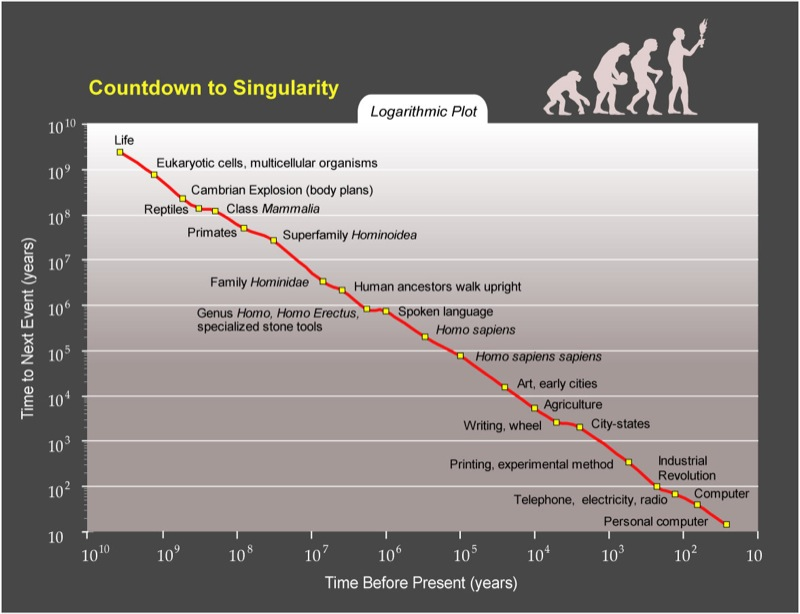
\includegraphics[width=0.618\textwidth]{pictures/sozlog}
\end{center}
\caption{Countdown to Singularity}\label{sozlog}
\end{figure}

\listoffigures
%\listoftables
%\newpage
%\nocite{*}
%\bibliographystyle{plain}
%\bibliography{preamble/literaturgoogle}
\end{document}